\documentclass[twoside, 11pt, titlepage]{article}

bookmark88�anag��LK+��Archi�Usersdavidepeccioli	DocumentsPersonal Knowledge Managementnote archiveuni
primo anno	unito.tex  8Lt���(�
�����n�%���b��� ��$4DTA�'���	file:///Macintosh HD� htA��$E81A49BF-F8E1-4658-8356-C54D8CF4E1D4���/3dnibtex????�����d�@�T�U�V� | � � 0     \0 ���� �������"��

\hypersetup{
    pdfauthor={Davide Peccioli},
    pdftitle={Geometria 1},
}

\begin{document}

\begin{titlepage}
\null
\vfill
\begin{center}
{\Huge \textbf{Geometria 1}}\\
\vspace{1em}
{\large Davide Peccioli}\\
\vspace{0.6em}
{\large Anno accademico 2021-2022}
\vfill
Università degli studi di Torino
\end{center}
\end{titlepage}
{\pagestyle{empty}
\null\newpage}

\tableofcontents\cleardoublepage

\section{Insiemi}\marginnote{20 set 2021}

Gli insiemi numerici a cui siamo abituati da sempre sono
\begin{gather*}
    \N=\{0, 1, 2, \cdots\}\\
    \Z=\{\cdots, -2, -1, 0, 1, 2, \cdots\}\\
    \Q=\{r=\frac{m}{n}:m \in \Z, n \in \N\setminus\{0\}, m,n \text{ primi tra loro}\}
\end{gather*}

Per l'insieme $ \Q $ esiste una rappresentazione decimale:
\[
    r=n,\alpha_1 \alpha_2 \alpha_3 \cdots\alpha_{j} \cdots
\]
con $ n \in \Z $, $ a_{i} \in\{0, 1, 2,\cdots,9\} $. "$ \alpha_1 \alpha_2 \alpha_3 \cdots\alpha_{j} \cdots $" prende il nome di allineamento periodico (o finisce o si ripete all'infinito).

\subsection{Corrispondenza biunivoca}

Due insiemi \textit{finiti} possono essere messi in corrispondenza biunivoca se e solo se hanno lo stesso numero di oggetti.

\subsubsection{Corrispondenza $ \N-\Z $}

\begin{center}
\begin{tikzpicture}
    \matrix (m) [matrix of math nodes,row sep=3em,column sep=0em,minimum width=0.3em]
    {
        \N=\{ & 0; & 1; & 2; & 3; & 4; & \dots &\dots\} \\
        \Z=\{ & \dots & -2; & -1; & 0; & 1; & 2; &\dots\}\\};
    \node [below] (n0) at (m-1-2) {};
    \node [below] (n1) at (m-1-3) {};
    \node [below] (n2) at (m-1-4) {};
    \node [below] (n3) at (m-1-5) {};
    \node [below] (n4) at (m-1-6) {};
    \node [above] (z-2) at (m-2-3) {};
    \node [above] (z-1) at (m-2-4) {};
    \node [above] (z0) at (m-2-5) {};
    \node [above] (z1) at (m-2-6) {};
    \node [above] (z2) at (m-2-7) {};
    \draw [<->] (n0) -- (z0);
    \draw [<->] (n1) -- (z1);
    \draw [<->] (n2) -- (z-1);
    \draw [<->] (n3) -- (z2);
    \draw [<->] (n4) -- (z-2);
    % \path[-stealth]
    %   (m-1-1) edge node [left] {} (m-2-4);
\end{tikzpicture}
\end{center}

\subsubsection{Corrispondenza $ \N - \N\times \N $}

In rosso è segnato l'insieme $ \N $, mentre in nero le coppie di $ \N\times \N$, che sono state ordinate dalle freccie rosse:
\begin{center}
    \begin{tikzpicture}
        \matrix (m) [matrix of math nodes,row sep=1em,column sep=1em,minimum width=0.3em]
        {
            00^{\textcolor{red}{1}} & 01^{\textcolor{red}{2}} & 02^{\textcolor{red}{6}} & 03^{\textcolor{red}{7}} & \dots\\
            10^{\textcolor{red}{3}} & 11^{\textcolor{red}{5}} & 12^{\textcolor{red}{8}} & 13 & \dots\\
            20^{\textcolor{red}{4}} & \dots & \dots & \dots & \dots \\
            \vdots & \vdots & \vdots & \vdots & \ddots\\};
        \node [right] (00) at (m-1-1) {};
        \node [left] (01a) at (m-1-2) {};
        \node [below left] (01b) at (m-1-2) {};
        \node [above right] (10a) at (m-2-1) {};
        \node [below] (10b) at (m-2-1) {};
        \node [above] (20a) at (m-3-1) {};
        \node [above right] (20b) at (m-3-1) {};
        \node [below left] (11a) at (m-2-2) {};
        \node [above right] (11b) at (m-2-2) {};
        \node [below left] (02a) at (m-1-3) {};
        \node [right] (02b) at (m-1-3) {};
        \node [left] (03a) at (m-1-4) {};
        \node [below left] (03b) at (m-1-4) {};
        \node [above right] (12a) at (m-2-3) {};
        \node [below left] (12b) at (m-2-3) {};
        \node [above right] (dd) at (m-3-2) {};
        
        \draw [->, red] (00) -- (01a);
        \draw [->, red] (01b) -- (10a);
        \draw [->, red] (10b) -- (20a);
        \draw [->, red] (20b) -- (11a);
        \draw [->, red] (11b) -- (02a);
        \draw [->, red] (02b) -- (03a);
        \draw [->, red] (03b) -- (12a);
        \draw [red, dotted, thick] (12b) -- (dd);
    \end{tikzpicture}
    \end{center}

In generale, se $ K \leftrightarrow \N $ (dove $ \leftrightarrow $ si legge "in corrispondenza biunivoca") $\implies$ 
\begin{align*}
    K & \leftrightarrow K\times K = K^{2} \\
    K & \leftrightarrow K\times K \times K = K^{3} \\
    K & \leftrightarrow K\times K\times\cdots\times K = K^{n} \\
\end{align*}

\definizione{}{Un insieme $ A $ è detto \textit{numerabile} se può essere messo in corrispondenza biunivoca con $ \N $}

Gli insiemi $ \N $, $ \Z $, $ \Q $ e $ \N^{n} $, $ \Z^{n} $, $ \Q^{n} $ sono numerabili
\fancypagestyle{ciccio}
{
	\renewcommand{\headrulewidth}{0pt}
    \fancyhead[LE, RO]{\underline{21 settembre 2021}}
}

\thispagestyle{ciccio}

\section{Operazioni con le matrici}
\subsection{Moltiplicazione}

Si può moltiplicare $\lambda \in \R$ con matrici $A\in\rmn$
\[
\lambda A=\lambda\qmatrice{a}=\qmatrice{\lambda a}
\]
\[
-1\cdot A = -A\qquad\text{coerente con la definizione di }-A
\]

\esempio{
\[
2\begin{pmatrix}
3 & 1 & 0\\
-1 & 4 & 1
\end{pmatrix}=\begin{pmatrix}
6 & 2 & 0\\
-2 & 8 & 2
\end{pmatrix}
\]
}

\osservazione{$0\cdot A$ è la matrice nulla $\forall A\in \rmn$}

\proprieta[del prodotto per scalari]{
\begin{itemize}
\item [(\textit{i})] $\displaystyle \lambda(A+B)=\lambda A + \lambda B \qquad\forall\lambda\in\R,\:A,B\in\rmn$
\item [(\textit{ii})] $\displaystyle (\lambda+\mu)\cdot A=\lambda\cdot A+\mu\cdot A\qquad\forall\lambda\mu\in\R,\:A\in\rmn$
\item [(\textit{iii})] $\displaystyle(\lambda\mu)A=\lambda(\mu A)\qquad\forall\lambda\mu\in\R,\:A\in\rmn$
\item [(\textit{iv})] $\displaystyle 1\cdot A = A\qquad\forall A\in\rmn$
\end{itemize}
}

$(\rmn, +)$ è un \textbf{gruppo abeliano} in cui è definita una moltiplicazione per scalari in cui valgono le proprietà \textit{i}-\textit{iv} (prototipo per gli spazi vettoriali).

\subsection{Prodotto tra matrici}
\[
A,B\:\tc\: A\in\R^{m,\textcolor{red}{n}}, B\in\R^{\textcolor{red}{n}, k}\implies AB\in \R^{m, k}
\]
Questo è definito come il prodotto \textbf{righe per colonne}. Il numero di colonne della prima matrice deve corrispondere con il numero di righe della seconda matrice.

\definizione{
	Siano $ A \in \R^{m,n} $ e $ B \in \R^{n,k} $ due matrici, siano $ a_{ij}  $ gli elementi di $ A $ e $ b_{rs}  $ gli elementi di $ B $ [Notazione: $ A=(a_{ij})$, $ B=(b_{rs}) $]

	La matrice $ A\cdot B $ è la matrice in $ R^{m,k} $ il cui $ ij $-esimo elemento è
	\[
		a_{i1} \cdot b_{1j} + a_{i 2} \cdot b_{2j} + \cdots+ a_{in} \cdot b_{ni} =\sum_{r=1}^n a_{ir} \cdot b_{rj}  
	\]
}

\subsubsection{Prodotto tra matrici quadrate}

Siano $ A, B \in \R^{m,m} $, $ AB \in \R^{m,m} $; in questo caso il prodotto tra matrici definisce una operazione in $ \R^{m,m} $.
\begin{itemize}
	\item [\textit{i}.] il prodotto è associativo: $ (A\cdot B) \cdot C = A \cdot (B\cdot C) $, $ \forall A, B, C \in \R^{m,m} $
	\item [\textit{ii}.] esiste un elemento neutro
\end{itemize}

\proposizione{matrid}{
	Sia $ I \in \R^{m,m} $ la matrice identità, $ A \in \R^{m,m} $ 
	
	$\implies$ $ A\cdot I = I\cdot A = A $ $ \forall A \in \R^{m,m} $
}
\dimostrazioneprop{matrid}{
	Sia $ (r_{ij} ) $ l'$ij$-esimo elemento della matrice $ A\cdot I $ con $ A=(a_{ij} ) $ e $ I = (b_{ij} ) $ \[
		r_{ij} = \sum_{n=1}^m a_{in}\cdot b_{ni}  
	\]
	Si noti che $ b_{kh} =0 $ $ \forall k,h | k \neq h $ $\implies$ 
	\begin{multline*}
		r_{ij} = \sum_{n=1}^m a_{in}\cdot b_{ni}  =\\
		= \cancel{a_{i1}b_{1j}}  + \cancel{\cdots} + a_{ij}b_{jj}+ \cancel{\cdots}+\cancel{a_{in}b_{nj}}=\\
		=a_{ij} \cdot b_{jj} = a_{ij} \cdot 1     
	\end{multline*} 
	
	$\implies$ $ r_{ij}=a_{ij}$
}

In generale se $ A \in \R^{m,m} $ $ \nexists $ un inverso per $ A $, cioè non esiste $ B \in \R^{m,m} $ tale che $ A \cdot B = B \cdot A = I $

\esempio{
	\begin{itemize}
		\item Se $ A $ è la matrice nulla 
		
		$\implies$ $ A \cdot B = $ matrice nulla $ \neq I $
		\item Se $ A $ ha una riga o una colonna nulla (ovvero fatta tutta di zeri)
		
		$\implies$ non è invertibile
	\end{itemize}
}

\section{Lipsum 1}
\lipsum

\part{Funzioni e Successioni}
\section{Corrispondenze}
Siano\marginnote{5 ott 2021} $ X, Y $ insiemi, e consideriamo $ P(x,y) $ predicato su $ x \in X $ e su $ y \in Y $.
\esempi{}{
    \begin{itemize}
        \item $X$: fantini di una squadra\\ $Y$: cavalli della stessa squadra\\ $ P(x,y) $: $ x $ ha cavalcato almeno una volta $ y $;
        \item $ X=Y= \R $; $ P(x,y) $: $ x^{2}+y^{2}=1 $;
        \item $ X=Y= \R $; $ P(x,y) $: $ y=x^{2} $.
    \end{itemize}
}

\definizione{}{Una \textit{corrispondenza} $ \mathfrak{F} $ tra gli elementi di $ X $ e di $ Y $ è un predicato binario $ P(x,y) $ nelle variabili $ x \in X $, $ y \in Y $.

Diciamo che $ x \in X $ è in corrispondenza con $ y \in Y $ se $ P(x,y) $ è verificata. Scriviamo \[
    y=\mathfrak{F} (x)
\]}

\definizione{}{
    Sia $ \mathcal{R}  $ il \textit{sottoinsieme} di $ X\times Y $ costituito dalle coppie $(x,y)$ per cui la relazione è vera \[
        \mathcal{R} =\{(x,y) \in X\times Y\,|\, P(x,y)\text{ è verificata}\} \subseteq X\times Y
    \]
    $ \mathfrak{F}  $ è univocamente determinata da $ \mathcal{R}  $.

    $ \mathcal{R}  $ prende il nome di \textit{grafo} (o grafico) di $ \mathfrak{F}  $. Una corrispondenza è totalmente individuata dal grafo.
}

\esempio{}{
    $ X=Y= \R $, \begin{align*}
        \mathfrak{F}:\R & \to \R \\
    x & \mapsto y=\mathfrak{F}(x)\quad\text{ se } x^{2}+y^{2}=1
    \end{align*} \[
        \mathcal{R} =\{(x,y) \in \R^{2}\,|\, x^{2}+y^{2}=1\}
    \]
    \begin{center}
    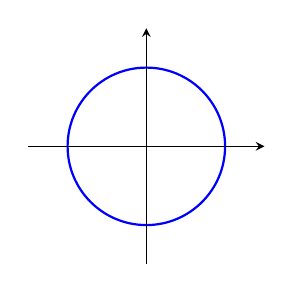
\begin{tikzpicture}
        \draw [blue, thick] (0,0) circle (1);
        \draw [-stealth] (-1.5, 0) -- (1.5, 0);
        \draw [-stealth] (0, -1.5) -- (0, 1.5);
    \end{tikzpicture}
    \end{center}
}
\begin{minipage}{\textwidth}
    \osservazione{
    Si noti come in questo esempio, 

    \vspace{0.5em}
    \begin{multicols}{2}
        \begin{align*}
        \frac{1}{2}&\to \frac{\sqrt{3}}{2}\\
        \frac{1}{2}&\to \frac{-\sqrt{3}}{2}
        \end{align*}
    \begin{center}
        \columnbreak

        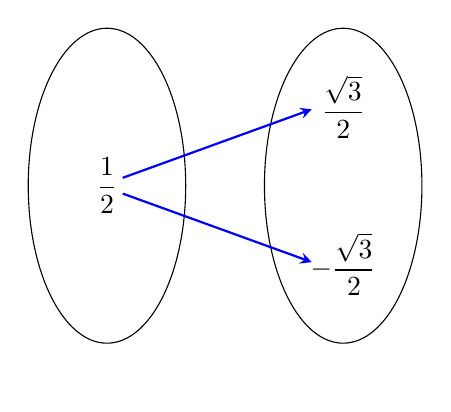
\begin{tikzpicture}
            \draw (-1.5,0) ellipse (1 and 2);
            \draw (1.5,0) ellipse (1 and 2);
            \node at (-1.5, -2.4) {$\R$};
            \node at (1.5, -2.4) {$\R$};
            \node at (-1.5, 0) {$\displaystyle%
            \frac{1}{2}$};
            \node at (1.5, 1) {$\displaystyle%
            \frac{\sqrt{3}}{2}$};
            \node at (1.5, -1) {$\displaystyle%
            -\frac{\sqrt{3}}{2}$};
            \draw [blue, thick, -stealth] (-1.3, 0.1) -- (1.1, 0.97); 
            \draw [blue, thick, -stealth] (-1.3, -0.1) -- (1.1, -0.97); 
        \end{tikzpicture}
    \end{center}
    \end{multicols}
    Mentre in altri casi, come \begin{align*}
    \mathscr{G} :\R & \to \R \\
    x & \mapsto x^{2}
    \end{align*} con \[
        \mathcal{R} =\{(x,y) \in \R^{2}\,|\, y=x^{2}\}
    \] vale \begin{equation}
        \forall\, x \in X=\R\quad \exists!\, y \in Y=\R\,\tc\, y=\mathscr{G} (x)\label{proprieta1}
    \end{equation}
}
\end{minipage}

\esempio{
    Sia $ X $ l'insieme dei fantini e $ Y $ l'insieme dei cavalli. $ Y= \mathscr{L}(x) $ se $ x  $ ha cavalcato almeno una volta $ y $. La corrispondenza può avere una forma simile:
    \begin{center}
        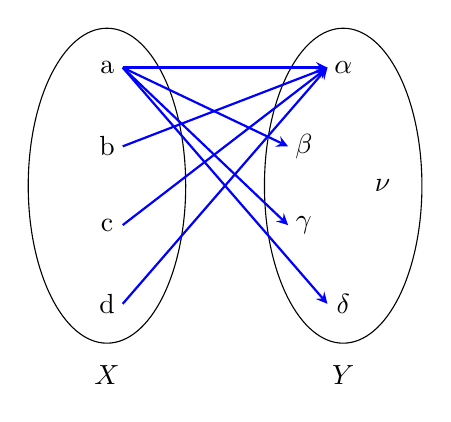
\begin{tikzpicture}
            \draw (-1.5,0) ellipse (1 and 2);
            \draw (1.5,0) ellipse (1 and 2);
            \node at (-1.5, -2.4) {$X$};
            \node at (1.5, -2.4) {$Y$};
            \node at (-1.5, 1.5) {a};
            \node at (-1.5, 0.5) {b};
            \node at (-1.5, -0.5) {c};
            \node at (-1.5, -1.5) {d};
            \node at (1.5, 1.5) {$\alpha$};
            \node at (1, 0.5) {$\beta$};
            \node at (1, -0.5) {$\gamma$};
            \node at (1.5, -1.5) {$\delta$};
            \node at (2, 0) {$\nu$};
            \draw [blue, thick, -stealth] (-1.3, 1.5) -- (1.3, 1.5); 
            \draw [blue, thick, -stealth] (-1.3, 1.5) -- (0.8, 0.5); 
            \draw [blue, thick, -stealth] (-1.3, 1.5) -- (0.8, -0.5); 
            \draw [blue, thick, -stealth] (-1.3, 1.5) -- (1.3, -1.5); 
            \draw [blue, thick, -stealth] (-1.3, 0.5) -- (1.3, 1.5); 
            \draw [blue, thick, -stealth] (-1.3, -0.5) -- (1.3, 1.5); 
            \draw [blue, thick, -stealth] (-1.3, -1.5) -- (1.3, 1.5); 
        \end{tikzpicture}
    \end{center}
    In questo caso la proprietà \eqref{proprieta1} non è soddisfatta.
}

Si nota che vi è una sostanziale differenza tra $ \mathscr{L} $ e $ \mathscr{G} $

\section{Funzioni}
\definizione{}{Una corrispondenza $ \mathscr{G} $:
    \begin{align*}
    \mathscr{G}: X & \to Y \\
     & x \mapsto y=\mathscr{G}(x)
    \end{align*} è una  textit{funzione} se $ \forall\,x \in X $ esiste al più un $ y \in Y $ tale che $ y=\mathscr{G}(x) $.
}

Nel corso si utilizzeranno sempre funzioni \begin{align*}
f:\R^{m} & \to \R^{n} \\
x & \mapsto y=f(x)
\end{align*}

\subsection{Definizioni}

\definizione{}{
    $ D \subseteq \R^{m} $ è detto \textit{dominio} di $ f $ se \[
        \forall\, x \in D\quad \exists\, y \in \R^{n}\,\tc\, y=f(x)
    \]

    Se non meglio specificato, $ D $ è dato da tutti gli $ x \in \R^{m} $ per cui l'espressione $ y =f(x) $ ha significato.
}
%DOMANDA: nella scrittura f:X\to Y, X è il dominio e Y è il codominio, vero? A questo punto, non è sbagliato scrivere log x: R\to R? Non andrebbe scritto log x: D\to R, specificando successivamente il dominio?
\definizione{}{Data una funzione \begin{align*}
f:X & \to Y \\
x & \mapsto y
\end{align*} si definisce \textit{codominio} di $ f $ l'insieme $ Y $.}
\esempio{}{
    $ f(x)=\ln (x-1) $, $ f: \R\to \R $. Deve valere $ x-1>0 $, pertanto \[
        D=(1, +\infty)=\{x \in \R\,|\, x>1\}
    \]
}
\notazione{}{
    Indichiamo \[
        D=\dom f
    \]
}
\esempio{}{
    Sia $ v=v(t) $ la velocità all'istante $ t $ di un corpo in caduta libera con velocità iniziale nulla.
    $ D \subseteq \R $ \begin{align*}
    v:D & \to \R \\
    t & \mapsto v(t)=g\,t
    \end{align*} con $ g $ accelerazione. Si noti che $ D\neq \R $, in quanto $ t $ è un tempo, e pertanto deve essere $ t\ge 0 $, allora \[
        D=[0, +\infty)=\{t \in \R; t\ge 0\}
    \]
}
\attenzione{Il dominio $ D=\dom f $ fa parte integrante della definizione della funzione, e deve essere sempre indicato.}
\esempio{}{\phantomsection\label{esempiofuncin}
        \begin{align*}
        f:\R &\to \R & g:[0; + \infty) &\to \R\\
        x & \mapsto y=x^{2} &  x &\mapsto y=x^{2}\\
        \dom f &= \R & \dom g &= [0; + \infty)
        \end{align*} 
        
        Si noti che \begin{align*}
            \graph (f)&=\{(x,y) \in \R\,|\, y=x^{2}\}\\ \graph (g)&=\{(x,y) \in [0; + \infty)\,|\, y=x^{2}\}
        \end{align*}

        $ f $ e $ g $ sono funzioni diverse.
}

\subsection{Funzioni iniettive, suriettive e biiettive}
\definizione{Data una funzione $ g:D\to Y $, $ f $ è \textit{iniettiva} se \begin{equation}
        \forall\,x_1, x_2 \in \dom g\qquad \begin{aligned}
            g(x_1)=g(x_2) \,&\implies\,x_1=x_2\\
            \big(x_1\neq x_2 \,&\implies\, g(x_1)\neq g(x_2)\big)
        \end{aligned}
    \end{equation}
}
\osservazione{}{
    La funzione $ g $ dell'\hyperref[esempiofuncin]{esempio (\thesection.\theesempi)} è iniettiva.
}
\definizione{}{
    Data $ f:D\to Y $, $ D=\dom f $, diciamo \textit{immagine} di $ f $ \begin{equation}
        f(D)=\im (f)=\bigl\{y \in Y\,\tc\quad \exists\, x \in D\,|\, y =f(x)\bigl\}
    \end{equation}
}
\definizione{}{
    Diciamo che \begin{align*}
    f:D & \to Y \\
    x & \mapsto f(x)
    \end{align*} è \textit{suriettiva} se \begin{equation}
        \forall\, y \in Y\quad \exists\, x \in D\,\tc\, y=f(x)
    \end{equation}
}

Una funzione $ f:D\to f(D) $ è sempre suriettiva.

\definizione{}{Diciamo che $ f: D\to Y $ è \textit{biettiva} (biunivoca) se è sia suriettiva che iniettiva.}

\subsection{Funzione composta}

Siano $ X, Y, W $ insiemi generici, e siano \begin{gather*}
    \begin{aligned}
        f: D &\to Y\\
        x &\mapsto y =f(x)
    \end{aligned}\qquad D=\dom f \subseteq X\\
    \begin{aligned}
        g: D' &\to w\\
        y &\mapsto w =g(x)
    \end{aligned}\qquad D'=\dom g \subseteq Y
\end{gather*}

Assumendo $ f(D) \subseteq D' $, possiamo costrure $ F $:
\begin{center}
    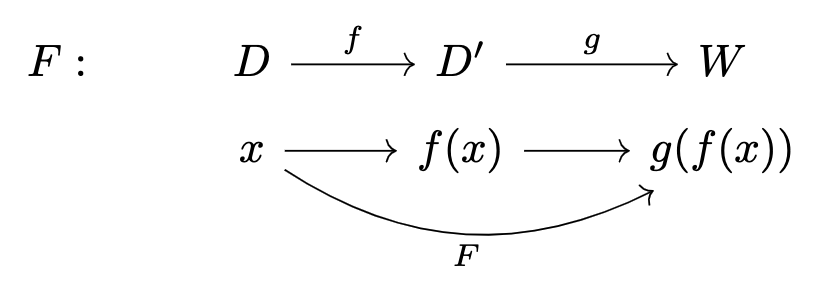
\includegraphics[width=7cm]{1.png}
\end{center}

La funzione \begin{align*}
F:D & \to W \\
x & \mapsto F(x)=g\bigl(f(x)\bigr)
\end{align*} è detta \textit{funzione composta} di $ f $ e $ g $. Si indica \[
    F=g\circ f
\]
\esempio{}{
    Siano $ D, D' \subseteq \R $, \[
        \begin{aligned}
            f: D&\to \R\\
            x &\mapsto x^{2}
        \end{aligned}\hspace{4em}\begin{aligned}
            g: D' &\to \R\\
            x&\mapsto \sqrt{x}
        \end{aligned}
    \]
    \vspace{1em}

    \begin{multicols}{2}
        \begin{center}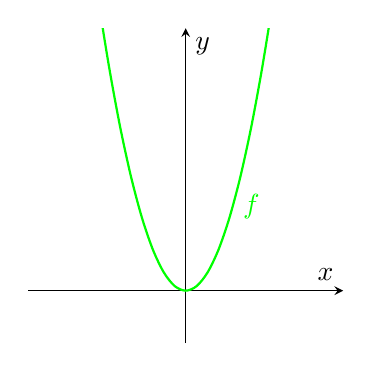
\begin{tikzpicture}\begin{axis}[
                xlabel=$x$,
                ylabel=$y$,
                axis equal,
                axis lines=middle,
                enlargelimits,
                xmax=5,
                xmin=-5,
                ymax=9,
                ymin=-1,
                xtick={0},
                ytick={0},
                scale only axis, 
                height=4cm, 
                width=4cm
                ]
            \addplot [no marks, green, smooth, thick, x=-1:5] {x^2};
            \node at (2.5, 3.2) {\textcolor{green}{$f$}};
        \end{axis}\end{tikzpicture}\end{center}
        \columnbreak

        \begin{center}
        \begin{tikzpicture}
            \begin{axis}[
                xlabel=$x$,
                ylabel=$y$,
                axis equal,
                axis lines=middle,
                enlargelimits,
                xmax=5,
                xmin=-1,
                ymax=5,
                ymin=-1,
                xtick={0},
                ytick={0},
                scale only axis, 
                height=4cm, 
                width=4cm
                ]
                \addplot [no marks, blue, smooth, thick, domain=0:5] {x^0.5};
                \node at (1, 1.6) {\textcolor{blue}{$g$}};
            \end{axis}
        \end{tikzpicture}\end{center}
    \end{multicols}
    

    Sia ha $ D=\dom f=\R $, $ D'=\dom g=[0, + \infty) $. Inoltre \[
        f(D)=[0, + \infty) \subseteq \dom g
    \] \begin{align*}
    g\circ f:\R & \to [0, + \infty) \\
    x & \mapsto \sqrt{x^{2}}=|x|
    \end{align*}

    Vale $ \dom f= \R $, $ \dom g=[0, + \infty) $, $ \dom (g\circ f)= \R $

    \begin{center}
    \begin{tikzpicture}
        \begin{axis}[
            xlabel=$x$,
            ylabel=$y$,
            axis equal,
            axis lines=middle,
            enlargelimits,
            xmax=5,
            xmin=-5,
            ymax=5,
            ymin=-1,
            xtick={0},
            ytick={0},
            scale only axis, 
            height=4cm, 
            width=6cm
            ]
            \addplot [no marks, red, smooth, thick, domain=-5:0] {-x};
            \addplot [no marks, red, smooth, thick, domain=0:5] {x};
            \node at (1, 2.3) {\textcolor{red}{$g\circ f$}};
        \end{axis}
    \end{tikzpicture}\end{center}
}   
\esempio{}{
    \[
        \begin{aligned}
            D& \subseteq \R^{2}\\
            f:D & \to \R^{2} \\
            x=(x_1,x_2) & \mapsto y=(x_1^{2},x_2^{2})
        \end{aligned}\qquad
        \begin{aligned}
            D'& \subseteq \R^{2}\\
            g:D' & \to \R \\
            x=(x_1,x_2) & \mapsto y=\sqrt{x_1+x_2}
        \end{aligned}
    \]
    Vale: $ D=\dom f=\R^{2} $ \[
        \im (f)=[0, + \infty)\times [0, + \infty)
    \]
    \begin{center}
        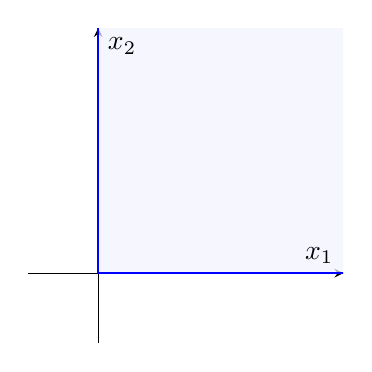
\begin{tikzpicture}
            \begin{axis}[
                xlabel=$x_1$,
                ylabel=$x_2$,
                axis equal,
                axis lines=middle,
                enlargelimits,
                xmax=5,
                xmin=-1,
                ymax=5,
                ymin=-1,
                xtick={0},
                ytick={0},
                scale only axis, 
                height=4cm, 
                width=4cm
                ]
                \addplot [no marks, blue, thick, fill=blue!5, fill opacity=0.7] coordinates {(0,0) (0,7) (7,7) (7, 0) (0,0)};
            \end{axis}
        \end{tikzpicture}\end{center}

        Inoltre \[
            D'=\dom g=\{(x_1, x_2) \in \R^{2}\,|\, x_1+x_2\ge 0\}
        \]
        \begin{center}
            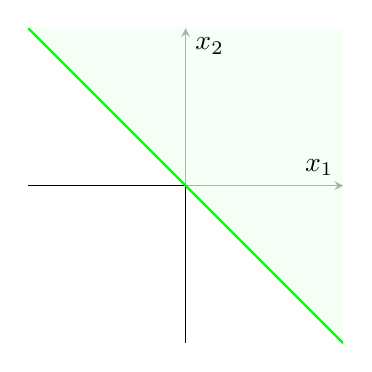
\begin{tikzpicture}
                \begin{axis}[
                    xlabel=$x_1$,
                    ylabel=$x_2$,
                    axis equal,
                    axis lines=middle,
                    enlargelimits,
                    xmax=5,
                    xmin=-5,
                    ymax=5,
                    ymin=-5,
                    xtick={0},
                    ytick={0},
                    scale only axis, 
                    height=4cm, 
                    width=4cm
                    ]
                    \addplot [no marks, green, thick, fill=green!5, fill opacity=0.7] coordinates {(-7,7) (7,-7) (7,7) (-7, 7)};
                \end{axis}
            \end{tikzpicture}\end{center}

            Quindi $ \im(f) \subseteq \dom g $ \begin{align*}
            g\circ f:\R^{2} & \to \R \\
            x=(x_1,x_2) & \mapsto \sqrt{x_1^{2}+x_2^{2}}=|x|
            \end{align*}
            \begin{center}
                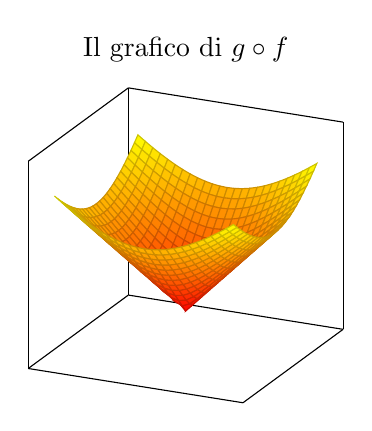
\begin{tikzpicture}
                    \begin{axis}[
                        xlabel=,
                        ylabel=,
                        zlabel=,
                        axis equal,
                        enlargelimits,
                        xmax=5,
                        xmin=-5,
                        ymax=5,
                        ymin=-5,
                        xtick=\empty,
                        ytick=\empty,
                        ztick=\empty,
                        scale only axis, 
                        height=4cm, 
                        width=4cm,
                        view={25}{20},
                        title={Il grafico di $ g\circ f $}
                        ]
                        \addplot3 [no marks, surf,
                        colormap/redyellow] ({x}, {y}, {(x^2 + y^2)^0.5});
                    \end{axis}
                \end{tikzpicture}\end{center}

}
\esempio{}{
    \[
        \begin{aligned}
            D& \subseteq \R\\
            f:D & \to \R \\
            x & \mapsto x^{2}
        \end{aligned}\hspace{3em}
        \begin{aligned}
            D'& \subseteq \R\\
            g:D' & \to \R \\
            x & \mapsto \ln x
        \end{aligned}
    \]
    Si ha $ D=\dom f=\R $, $ D'=\dom g =(0, + \infty) $

    \begin{multicols}{2}
        \begin{center}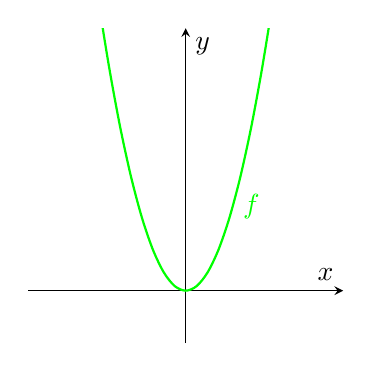
\begin{tikzpicture}\begin{axis}[
                xlabel=$x$,
                ylabel=$y$,
                axis equal,
                axis lines=middle,
                enlargelimits,
                xmax=5,
                xmin=-5,
                ymax=9,
                ymin=-1,
                xtick={0},
                ytick={0},
                scale only axis, 
                height=4cm, 
                width=4cm
                ]
            \addplot [no marks, green, smooth, thick, x=-1:5] {x^2};
            \node at (2.5, 3.2) {\textcolor{green}{$f$}};
        \end{axis}\end{tikzpicture}\end{center}
        \columnbreak

        \begin{center}
        \begin{tikzpicture}
            \begin{axis}[
                xlabel=$x$,
                ylabel=$y$,
                axis equal,
                axis lines=middle,
                enlargelimits,
                xmax=5,
                xmin=-1,
                ymax=5,
                ymin=-1,
                xtick={1},
                ytick={0},
                scale only axis, 
                height=4cm, 
                width=4cm
                ]
                \addplot [no marks, blue, smooth, thick, domain=0:5] {ln(x)};
                \node at (3, 1.7) {\textcolor{blue}{$g$}};
            \end{axis}
        \end{tikzpicture}\end{center}
    \end{multicols}

    Dal momento che $ f(D)=[0, + \infty) \nsubseteq D' $ non possiamo costruire $ g \circ f $. Restringiamo $ f $: \begin{align*}
    \tilde{f}:\R\setminus\{0\} & \to \R \\
    x & \mapsto x^{2}
    \end{align*} $ \tilde{f}(D)=(0,+ \infty) \subseteq\dom g $ \begin{align*}
    g\circ\tilde{f}:\R\setminus\{0\} & \to \R \\
    x & \mapsto \ln(x^{2})
    \end{align*}

    \begin{center}
        \begin{tikzpicture}
            \begin{axis}[
                xlabel=$x$,
                ylabel=$y$,
                axis equal,
                axis lines=middle,
                enlargelimits,
                xmax=5,
                xmin=-5,
                ymax=5,
                ymin=-1,
                xtick={0},
                ytick={0},
                scale only axis, 
                height=4cm, 
                width=6cm
                ]
                \addplot [no marks, red, unbounded coords=jump, thick] {ln(x^2)};
                \node at (1.4, 2.3) {\textcolor{red}{$\ln(x^{2})$}};
            \end{axis}
        \end{tikzpicture}\end{center}
}
\subsection{Funzione inversa}

Siano $ X, Y $ insiemi generici, $ D \subseteq X $. Se $ f:D\to Y $ è iniettiva, allora \[
    f:D\to f(D)
\] è \textit{biunivoca}, ovvero \begin{equation}
    \forall\,y \in f(D)\quad \exists!\, x \in D\quad y=f(x)
\end{equation}

Diciamo che $ f $ tra $ D $ e $ f(D) $ è \textit{invertibile}. Diciamo \textit{funzione inversa} di $ f $ \begin{align*}
\varphi:f(D) & \to D \\
y & \mapsto \varphi(y)=x
\end{align*} dove $ x $ è l'unico elemento di $ D $ tale che $ y=f(x) $. Si ha allora 
\[
    \begin{aligned}
        \varphi\circ f: D&\to D\\
        \dom f&\to \dom f\\
        x &\mapsto \varphi\circ f(x)=x
    \end{aligned}\hspace{4em}\begin{aligned}
        f\circ\varphi: f(D) &\to f(D)\\
        y&\mapsto f\circ\varphi(y)=y
    \end{aligned}
\] ossia \begin{equation}
    \varphi \circ f =\Id_{D} \qquad f\circ\varphi = \Id_{f(D)} 
\end{equation} dove $ \Id_{D}  $ è l'identità in $ D $ e $ \Id_{f(D)}  $ è l'identità in $ f(D) $.

La funzione inversa $ \varphi $ in genere si indica con $ f^{-1} $: \[
    f^{-1} \circ f =\Id_{D} \qquad f\circ f^{-1} = \Id_{f(D)}
\]
\esempio{}{
    \begin{align*}
    f:[0, + \infty) & \to [0, + \infty) \\
    x & \mapsto x^{2}
    \end{align*} $ \dom f =[0, + \infty) $: $ f  $ è biunivoca e dunque invertibile \begin{align*}
    f^{-1}:[0, + \infty) & \to [0, + \infty) \\
    x & \mapsto f^{-1}(x)= \sqrt{x}
    \end{align*}

    \begin{multicols}{2}
        \begin{center}\begin{tikzpicture}\begin{axis}[
                xlabel=$x$,
                ylabel=$y$,
                axis equal,
                axis lines=middle,
                enlargelimits,
                xmax=5,
                xmin=-5,
                ymax=9,
                ymin=-1,
                xtick={0},
                ytick={0},
                scale only axis, 
                height=4cm, 
                width=4cm
                ]
            \addplot [no marks, green, smooth, thick, domain=0:5] {x^2};
            \node at (2.5, 3.2) {\textcolor{green}{$f$}};
        \end{axis}\end{tikzpicture}\end{center}
        \columnbreak

        \begin{center}
        \begin{tikzpicture}
            \begin{axis}[
                xlabel=$x$,
                ylabel=$y$,
                axis equal,
                axis lines=middle,
                enlargelimits,
                xmax=5,
                xmin=-1,
                ymax=5,
                ymin=-1,
                xtick={0},
                ytick={0},
                scale only axis, 
                height=4cm, 
                width=4cm
                ]
                \addplot [no marks, blue, smooth, thick, domain=0:5] {x^0.5};
                \node at (1, 1.6) {\textcolor{blue}{$g$}};
            \end{axis}
        \end{tikzpicture}\end{center}
    \end{multicols}
    \begin{gather*}
        f^{-1}\circ f (x) = \sqrt{x^{2}}= x \qquad x\ge 0\\
        f \circ f^{-1}(x) = (\sqrt{x})^{2} = x\qquad x\ge 0
    \end{gather*}
}
\attenzione{
    Non confondere la funzione \textit{inversa} $ f^{-1} $ (ovvero tale che $f^{-1}\circ f =\id_{D} $) con la funzione \textit{reciproca} 
    \[
        [f(x)]^{-1}=\frac{1}{f(x)}
    \]
}

Nell'esempio precedente, funzione inversa e funzione reciproca sono ben diverse. Infatti, data \begin{align*}
f:[0,+ \infty) & \to [0, + \infty) \\
x & \mapsto x^{2}
\end{align*} vale che \[
    f^{-1}(x)=\sqrt{x}\qquad f(x)^{-1}=\frac{1}{x^{2}}
\] inoltre \[
    f \circ f^{-1}(x)=x\qquad f(x) \cdot f(x)^{-1}=1 \quad\forall\, x \in \R\setminus\{0\}
\]

\subsubsection{Grafico della funzione inversa}

\begin{center}
    \begin{tikzpicture}
        \begin{axis}[
            xlabel=$x$,
            ylabel=$y$,
            axis equal,
            axis lines=middle,
            enlargelimits,
            xmax=5,
            xmin=-1,
            ymax=5,
            ymin=-1,
            xtick={1},
            ytick={1},
            scale only axis, 
            height=7cm, 
            width=7cm,
            title={$f(x)=x^{2}\qquad x\ge 0$}
            ]
            \addplot [no marks, red, smooth, thick, domain=0:5] {x^0.5};
            \node at (4, 1.6) {\textcolor{red}{$f^{-1}(x)$}};
            \addplot [no marks, blue, smooth, thick, domain=0:5] {x^2};
            \node at (1.5, 4) {\textcolor{blue}{$f(x)$}};
            \addplot [no marks, green, dashed, thick] coordinates {(-3,-3) (7,7)};
        \end{axis}
    \end{tikzpicture}\end{center}

Il grafico di $ f^{-1} $ è il simmetrico del grafico di $ f $ rispetto alla bisettrice del primo e del terzo quadrante.

\esercizio{
    Verificare che la funzione $ f(x)=\sin x $ sia invertibile su $ \bigl[-\frac{\pi}{2}, +\frac{\pi}{2}\bigr] $, determinare il dominio dell'inversa e disegnare entrambi i grafici \[
        f^{-1}(x)=\arcsin x
    \]
}{
    Da risolvere %ESERCIZIO risolvere esercizio
}{}
\esercizio{
    Verificare che la funzione $ g(x)=\tan x $ è invertibile su $ \bigl(-\frac{\pi}{2}, +\frac{\pi}{2}\bigr) $, determinare dominio e grafico di $ g^{-1}(x) $ \[
        g^{-1}(x)=\arctan x
    \]
}{
    Da risolvere %ESERCIZIO risolvere esericizio
}{}

\subsection{Funzioni limitate}

Dato $ D \subseteq \R^{n} $,\begin{align*}
f:D & \to \R \\
x & \mapsto f(x)
\end{align*} è detta \textit{limitata} se $ f(D) $ è un insieme limitato, ossia \[
    \exists\, M>0\,\tc\quad \forall\, x \in D\qquad \begin{aligned}
        |f(x)|&<M\\
        -M<f(x)&< M
    \end{aligned}
\]

$ f $ è limitata superiormente (inferiormente) se \[
    \exists\, M>0\,\tc\quad \forall\, x \in D\qquad\begin{aligned}
        f(x)&<M\\
        \bigl(f(x)&>-M\bigr)
    \end{aligned}
\]

\esempio{}{
    \begin{align*}
    f:\R & \to \R \\
    x & \mapsto \sin x
    \end{align*} $ f $ è limitata in quanto $ f(D) \subseteq [-1, 1] $, ovvero \[
        \forall\, x \in \R\qquad -1\le f(x)\le 1
    \]
    \begin{center}
        \begin{tikzpicture}
            \begin{axis}[
                xlabel=$x$,
                ylabel=$y$,
                axis equal,
                axis lines=middle,
                enlargelimits,
                xmax=8,
                xmin=-8,
                ymax=2,
                ymin=-2,
                xtick={0},
                ytick={-1, 1},
                scale only axis, 
                height=4cm, 
                width=10cm]
                \addplot [no marks, blue, thick, samples=1000, domain=-8:8] {sin(x*180/3.1415)};
                \addplot [no marks, red, dashed, thick, domain=-8:8] {1};
                \addplot [no marks, red, dashed, thick, domain=-8:8] {-1};
            \end{axis}
        \end{tikzpicture}\end{center}
}
\definizione{}{
    Data $ f:D\to \R $, con $ D \subseteq \R $, diciamo \textit{estremo superiore} (inferiore) di $ f $ su $ D $ 
    \begin{align}
        \sup_{D} f &:= \sup\bigl(f(D)\bigr)\\
        \Bigl(\inf_{D} f &:= \inf\bigl(f(D)\bigr) \Bigr)
    \end{align} 
}
\esempio{Ecco due funzioni:

\begin{minipage}{\textwidth}
    \begin{multicols}{2}
        \begin{center}\begin{tikzpicture}\begin{axis}[
                xlabel=$x$,
                ylabel=$y$,
                axis equal,
                axis lines=middle,
                enlargelimits,
                xmax=5,
                xmin=-5,
                ymax=5,
                ymin=-5,
                xtick={0},
                ytick={0},
                scale only axis, 
                height=4cm, 
                width=4cm
                ]
            \addplot [no marks, green, smooth, thick, domain=-5:5] {x^3};
        \end{axis}\end{tikzpicture}\end{center} \begin{align*}
        f:\R & \to \R \\
        x & \mapsto x^{3}
        \end{align*}

        $ f $ non è limitata.
        \columnbreak

        \begin{center}
        \begin{tikzpicture}
            \begin{axis}[
                xlabel=$x$,
                ylabel=$y$,
                axis equal,
                axis lines=middle,
                enlargelimits,
                xmax=5,
                xmin=-1,
                ymax=5,
                ymin=-1,
                xtick={0},
                ytick={0},
                scale only axis, 
                height=4cm, 
                width=4cm
                ]
                \addplot [no marks, blue, smooth, thick, domain=0:5] {x^3};
\end{axis}\end{tikzpicture}\end{center}
\begin{align*}
g:[0,+\infty) & \to \R \\
x & \mapsto x^{3}
\end{align*} 

$ g $ è limitata inferiormente, e \[\inf_{[0,+ \infty)}  g =0=\min_{[0,+ \infty)}  g\]
\end{multicols}\end{minipage}}

\definizione{}{
    $ \sup f $ e $ \inf f$, se appartengono all'immagine $ f(D) $ sono detti \textit{valore massimo} e \textit{minimo} di $ f $.
}

\subsection{Massimi, minimi e monotonia}

Data $ f:D\to \R $, $ D \subseteq \R^{n} $, 
\begin{itemize}
\item $ x_0 \in D $ è \textit{punto di massimo} (\textit{minimo}) \textit{assoluto} o globale di $ f $ se \begin{equation}
    \forall\, x \in D\qquad \begin{aligned}
        f(x)&\le f(x_0)\\
        \bigl(f(x)&\ge f(x_0)\bigr)
    \end{aligned}
\end{equation}
\item $ x_0 $ è detto \textit{punto di massimo} (\textit{minimo}) \textit{locale} o relativo di $ f $ se \begin{equation}
    \exists\, U(x_0)\,\tc\quad \forall\, x \in U(x_0)\quad \begin{aligned}
        f(x)&\le f(x_0)\\
        \bigl(f(x)&\ge f(x_0)\bigr)
    \end{aligned}
\end{equation}
\item $ x_0 $ è detto \textit{punto di massimo} (\textit{minimo}) \textit{forte} di $ f $ se \begin{equation}
    \begin{aligned}
        \forall\, x &\in D\\
        \bigl(\exists\, U(x_0)\,\tc\quad \forall\, x &\in U(x_0)\bigr)
    \end{aligned}\qquad
     x\neq x_0\text{ si ha}\quad \begin{aligned}
        f(x)&< f(x_0)\\
        \bigl(f(x)&> f(x_0)\bigr)
    \end{aligned}
\end{equation}
\end{itemize}

\subsubsection{Funzioni monotone}   

Data $ f:D\to \R $, $ D \subseteq \R^{n} $, 
\begin{itemize}
\item $ f $ è \textit{crescente} (\textit{decrescente}) su $D $ se \begin{equation}
    \forall\, x_1, x_2 \in D\qquad x_1<x_2 \,\implies\, \begin{aligned}
        f(x_1)&\le f(x_2)\\
        \bigl(f(x_1)&\ge f(x_2)\bigr)
    \end{aligned}
\end{equation}
\item $ f $ è \textbf{strettamente} \textit{crescente} (\textit{decrescente}) su $D $ se \begin{equation}
    \forall\, x_1, x_2 \in D\qquad x_1<x_2 \,\implies\, \begin{aligned}
        f(x_1)&< f(x_2)\\
        \bigl(f(x_1)&> f(x_2)\bigr)
    \end{aligned}\end{equation}
\end{itemize}
\fancypagestyle{firststyle}
{
	\renewcommand{\headrulewidth}{0pt}
    \fancyhead[LE, RO]{\underline{7 ottobre 2021}}
}

\thispagestyle{firststyle}

\proposizione{somvet}{Sia $V$ uno spazio vettoriale e $W, W_1$ e $W_2$ sottospazi di $V$.

	Se $W$ contiene $W_1$ e $W$ contiene $W_2$ allora $W$ contiene $W_1+W_2$ (cioè $W_1+W_2$ è il più piccolo sottospazio di $V$ che contiene sia $W_1$ che $W_2$)}

\dimostrazioneprop{somvet}{Sia $x+y \in W_1+W_2$, $x \in W_1$ $\implies$ $x \in W, y \in W_2$ $\implies$ $y \in W$ $\implies$ $x+y \in W$, poiché $W$ è un sottospazio vettoriale. Quindi ogni $v \in W_1+W_2$ è elemento di $W$ $\implies$ $W_1+W_2 \subseteq W$.

La somma si generalizza a più sottospazi. Siano $W_1, \cdots, W_l \subseteq V$ sottospazi vettoriali, allora si definisce \[W_1+\cdots+W_l=\{x_1+\cdots+x_l | x_1 \in W_1, \cdots, x_l \in W_l\} \subseteq V\] è un sottospazio vettoriale ed è il più piccolo sottospazio che contiene tutti i $W_1,\cdots, W_l$}

\esercizio{
	Si trovino somma e intersezione dei seguenti sottospazi vettoriali di $\R^4$
	\begin{itemize}
		\item [a.] $W_1=\{(x_1, x_2, 0, 0) | x_1,x_2 \in \R\}$, $W_2=L(e_4)$
		\item [b.] $W_1=\{(x_1, x_2, 0, 0) | x:1,x:2 \in \R\}$,\\ $Z_2=\{(0, x_2, 0, x_4) | x_2, x_4 \in \R\}$
	\end{itemize}}{
	\begin{itemize}
		\item [a.] $W_1+W_2=\{(x_1, x_2, 0, x_4) | x_1, x_2, x_4 \in \R\}$, $W_1 \cap W_2=\{\underline{0}\}$
		\item [b.] $W_1+Z_2=\{(x_1, x_2, 0, x_4) | x_1, x_2, x_4 \in \R\}$,\\$W_1 \cap Z_2=\{(0, x_2, 0, 0) | x_2 \in \R\}$
	\end{itemize}}

\proposizione{caa}{Sia $V$ spazio vettoriale su un campo $\K$ e $W_1, W_2 \subseteq V$ due sottospazi. Sono fatti equivalenti le seguenti proposizioni:
	\numerato{\item $W_1 \cap W_2 = \{\underline{0}\}$ (hanno intersezione banale)
	\item ogni $v \in W_1+W_2$ si scrive in modo unico come $v=x+y$ con $x \in W_1$ e $y \in W_2$}}

\dimostrazioneprop{caa}{\elencop{\item [1. $\implies$ 2.] Suppongo $W_1 \cap W_2 = \{\underline{0}\}$ e considero $v \in W_1+W_2$. Scrivo $v=x_1+y_1$, $v=x_2+y_2$ e dimostro che $x_1=x_2$ e $y_1=y_2$

		$\underline{0}=v-v=(x_1+y_1)-(x_2+y_2)=(x_1-x_2)+(y_1-y_2)$ $\implies$ $x_1-x_2=y_2-y_1$, $x_1-x_2 \in W_1$ mentre $y_2-y_1 \in W_2$. Per l'uguaglianza risulta che 
		\[
		\begin{cases}
		x_1-x_2 \in W_2 \implies x_1-x_2 \in W_1 \cap W_2\\
		y_2-y_1 \in W_1 \implies y_2-y_1 \in W_1 \cap W_2
		\end{cases}\]
		\[
		\implies \begin{cases}
		x_1-x_2=\underline{0} \implies x_1=x_2\\
		y_2-y_1=\underline{0} \implies y_1=y_2
		\end{cases}\]
	
	\item [2. $\implies$ 1.] Suppongo che ogni $v \in W_1+W_2$ si scriva in modo unico come $v=x+y$ con $x \in W_1$ e $y \in W_2$ e dimostro che $W_1 \cap W_2 = \{\underline{0}\}$

		Sia $v \in W_1 \cap W_2$. Sia $v \in W_1+W_2$, $v=x+y=x+v+y-v$, con $x+v \in W_1$, $y-v \in W_2$. Quindi se $v \neq \underline{0}$, le due scritture $v=x+y$, $v=(x+v)+(y-v)$ sono diverse e ciò non è possibile per ipotesi}}

		
\notazione{
	Se $ W_1  \cap W_2 = \{\underline{0}\} $ si scrive $ W_1 \oplus W_2 $ invece che $ W_1+W_2 $
	$ \oplus $ si legge ``somma diretta''}
	
\esempio{ $\K^{n,n} = S(\K^{n,n}) \oplus A(\K^{n,n})$}
\esempio{$ R^2 = \mathscr{L}(e_1) \oplus \mathscr{L}(e_2) $}

\proposizione{vetteq}{
	Sia $ V $ uno spazio vettoriale su un campo $\K$. Siano $ W_1, \cdots, W_l \subseteq V $ sottospazi vettoriali. Sono fatti equivalenti le seguenti proposizioni
	\begin{enumerate}
	\item $ W_i \cap (W_1+\cdots+W_{i-1}+W_{i+1}+\cdots+W_l) =\{\underline{0}\} $ $ \forall i = 1,\cdots,l $
	\item Ogni $ v \in W_1+\cdots+W_l $ si scrive in modo unico come $ v=x_1+\cdots+x_l$ con $x_1 \in W_1, \cdots, x_l \in W_l$
	\end{enumerate}
	Se vale 1. si scrive $ W_1 \oplus W_2 \oplus \cdots \oplus W_l $}
	
%TODO Dimostrazione per esercizio

\esempio{
	Considero $ V $ spazio vettoriale di dimensione finita e $ \mathscr{B}=\{v1, \cdots, v_n\} $ $\implies$ $ V=\mathscr{L}(v_1) \oplus \cdots \oplus \mathscr{L}(v_l) $} %TODO controllare che l'esercizio sia finito

Sia $V$ spazio vettoriale su un campo $\K$, finitamente generato. Sia $ W \subseteq V $ un sottospazio vettoriale, sia $ \mathscr{B}=\{w_1, \cdots, w_l\} $ una base di $ W $. Possiamo completare $ \mathscr{B} $ con una base dello spazio $ \mathscr{B}'=\{w_1, \cdots, w_l, v_1, \cdots, v_m\} $. Sia \[ Z=\mathscr{L}(v_1,\cdots, v_m) \subseteq V\] un sottospazio vettoriale, e per costruzione $ V=W \oplus Z $

\osservazione{
	Sia $ V $ spazio vettoriale di dimensione finita con $ V=W \oplus Z $
	Siano $ \mathscr{B}=\{w1, \cdots, w_l\} $ una base di $ W $ e $ C=\{z_1, \cdots, z_m\} $ una base di $ Z $.
	Ogni elemento di $ V $ si scrive in modo unico come $ v=x+y $ con $ x \in W $ e $ y \in Z $
	$ \mathscr{B} $ base di $ W $ 
	
	$\implies$ $ x $ si scrive in modo unico come $ x=\lambda_1w_1+\cdots+\lambda_l w_l $
	
	$ \mathscr{C} $ base di $ Z $ $\implies$ $y$ si scrive in modo unico come \[ y=\mu_1z_1+\cdots+\mu_n z_n \]
	
	$\implies$ $ v $ si scrive in modo unico come \[v=\lambda_1w_1+\cdots+\lambda_l w_l+\mu_1z_1+\cdots+\mu_n z_n\]
	
	$\implies$ $ B \cup C=\{w1, \cdots, w_l, z_1, \cdots, z_l\} $ è una base di $ V  $
	
	$\implies$ $ \dim V = \dim W + \dim Z $}
	
\teorema{grassmann}{
	Sia $ V $ uno spazio vettoriale su un campo $\K$ finitamente generato. Siano $ W_1, W_2 \subseteq V $ due sottospazi vettoriali $ \tc V=W_1+W_2 $. Allora 
	\[\dim V = \dim W_1 + \dim W_2 - \dim (W_1 \cap W_2)\]
	Questa è la \textbf{Formula di Grassmann}.}
\dimostrazione{grassmann}{
Chiamo $ \dim V=n $, $ \dim W_1=l $, $ \dim W_2=p $, $ \dim (W_1 \cap W_2) = r $

In particolare $ l,p \leq n $, $ r\leq l,p $
\begin{enumerate}
    \item $ r=l $ $\implies$ $ W_1 \cap W_2 = W_1 $ $\implies$ $ W_1 \subseteq W_2 $ $\implies$ $ W_1+W_2=W_2=V $ %TODO mostrare tutte implicazioni
    \item $ r=p $ $\implies$ $ W_1 \cap W_2 = W_2 $ $\implies$ $ W_2 \subseteq W_1 $ $\implies$ $ W_1+W_1=W_1=V $ %TODO mostrare tutte le implicazioni
    \item si assume $ r\leq l,p $ e sia \[\mathscr{B}=\{a_1,\cdots,a_r\} \text{ base di } W_1 \cap W_2\]
    Completo $ \mathscr{B} $ con una base $ \mathscr{C} $ di $ W_1 $, \[\mathscr{C}=\{a_1, \cdots, a_r, b_{r+1}, \cdots, b_l\}\]e completo $ \mathscr{B} $ con una base $ \mathscr{D} $ di $ W_2 $, \[\mathscr{D}=\{a_1, \cdots, a_r, c_{r+1}, \cdots, c_p\}\]
    Si verifica che l'insieme \[\{a_1, \cdots, a_r, b_{r+1}, \cdots, b_l, c_{r+1}, \cdots, c_p\}\] è una base di $V$. In questo modo si ottiene \[\dim V= l + (p-r)\] cioè la tesi.
    
    Ovviamente risulta \[\mathscr{L}(a_1, \cdots, a_r, b_{r+1}, \cdots, b_l, c_{r+1}, \cdots, c_p)=V\] in quanto contiene i generatori sia di $W_1$ che di $W_2$, e quindi anche della loro somma. Verifichiamo che l'insieme \[\{a_1, \cdots, a_r, b_{r+1}, \cdots, b_l, c_{r+1}, \cdots, c_p\}\] sia libero.
    Supponiamo 
    \begin{multline*}\lambda_1a_1+ \cdots + \lambda_r a_r + \mu{r+1}+b_{r+1} + \cdots + \\ + \cdots + \mu_lb_l + \gamma_{r+1} c_{r+1} + \cdots + \gamma_p c_p = \underline{0}**\end{multline*}
    \[(\lambda_1a_1+ \cdots + \lambda_r a_r + \mu_{r+1} b_{r+1} + \cdots + \mu_l b_l)=( -\gamma_{r+1} c_{r+1} - \cdots - \gamma_p c_p)\]
    
    Sia \begin{multline*}c=(-\gamma_{r+1} c_{r+1} - \cdots - \gamma_p c_p)=\\=(\lambda_1a_1+ \cdots + \lambda_r a_r + \mu_{r+1} b_{r+1} + \cdots + \mu_l b_l)\end{multline*} sicuramente $c \in W_2$
    \[\lambda_1 a_1+ \cdots + \lambda_r a_r + \mu_{r+1} b_{r+1} + \cdots + \mu_l b_l \in W_1\] 
    
    $\implies$ $c \in W_1 \cap W_2 = \mathscr{L}(a_1,\cdots, a_r)$ \\
    
    $\implies$ $c = \beta_1 a_1 +\cdots+\beta_r a_r$, vado a sostituire in **
    \[(\beta_1 a_1 +\cdots+\beta_r a_r)+(\gamma_{r+1} c_{r+1} + \cdots + \gamma_p c_p) = \underline{0}\]
    \[\implies \begin{cases}
    	\beta_1=\cdots=\beta_r=0\\
    	\gamma_{r+1}=\cdots=\gamma_p=0
    \end{cases}\]	%TODO chiarire meglio perché

    Ho ottenuto
    \begin{gather*}
    \gamma_{r+1}=\cdots=\gamma_p=0\\
    \lambda_1a_1+ \cdots + \lambda_r a_r + \mu_{r+1} b_{r+1} + \cdots + \mu_l b_l=\underline{0}
    \end{gather*}
     
    Poiché l'insieme \[\mathscr{C}=\{a_1, \cdots, a_r, b_{r+1}, \cdots, b_l\}\] è libero
    
    $\implies$ $\lambda_1=\cdots=\lambda_r = \mu_{r+1}=\cdots=\mu_l=0$
    
    $\implies$ $\{a_1, \cdots, a_r, b_{r+1}, \cdots, b_l, c_{r+1}, \cdots, c_p\}$ è libero
\end{enumerate}}

%TODO sistemare appunti con quelli del prof
%TODO sistemare sistema di numerazione teoremi e proposizioni


\section{Lipsum 2}
\lipsum

\marginnote{2 nov 2021}

\section{Limite successione}

Data $ \{a_{n} \}_{n=0}^\infty, \N \to \R, a: n\to a_{n}  $, $l \in \R*$, diciamo che 
\[
    \lim_{n\to\infty}a_{n}=l  
\]
se $\forall V(l) \exists U(+\infty) n \in(\N intersezione D) \implies a_{n \in V(l)}$
Scriviamo $\forall V(l) \exists n_{segnato} \in N | \forall n>n_{segnato} a_{n} \in V(l)$

$l\in \R$, diciamo che $ \{a_{n} \}_{n=0}^\infty $ è \textbf{convergente} a $ l $ se $ \forall \varepsilon \exists n_{segnato} \in \N | \forall n>n_{segnato} |a_{n} -l |<\varepsilon  $

Se $ l=\pm \infty $ $a_{n}$ è divergente a $ \pm\infty $, se $ \lim_{n\to+\infty} a_{n}=\nexists $ allora $ \{a_{n}\}_{n=0 }^\infty$ è irregolare (o oscillante).


\esempio{
\begin{itemize}
    \item $ \{a_{n} \}_{n=0}^\infty=(-1)^n $ con $ n \in \N $ è irregolare e limitata
    \item $ \{b_{n} \}_{n=0}^\infty=(-1)^n\cdot n $ con $ n = 0, -1, 2, -3, 4, \cdots$ è irregolare e non limitata
\end{itemize}
}

Si dice di una successione $\{a_{n} \}_{n=0}^\infty$

\begin{itemize}
    \item $\forall \{a_{n} \}$ è crescente se $ \forall n \in \N $, $ a_{n} \le a_{n+1}  $
    \item $\forall\{a_{n} \}$ è strettamente crescente se $ \forall n \in \N $, $ a_{n} < a_{n+1}  $
    \item $\forall\{a_{n} \}$ è decrescente se $ \forall n \in \N $, $ a_{n} \ge a_{n+1}  $
    \item $\forall \{a_{n} \}$ è strettamente decrescente se $ \forall n \in \N $, $ a_{n} > a_{n+1}  $
\end{itemize}
Una successione crescente o decrescente si dice monotona, se strettamente crescente o decrescente si dice strettamente monotona.

Un predicato $ P(n) $ è verificato definitivamente se $ \exists n_{segnato} \forall n\le n_{segnato}$ $ P(n) $  è vero

Valgono per $ \{a_{n} \}_{n=0}^\infty$ i seguenti teoremi
\begin{itemize}
    \item Teorema di unicità del Limite
    \item Teorema di permanenza del segno 
    \item Teorema di limitatezza:
        \teorema{limitatezza}{
            \[
                \lim_{n\to \infty} a_{n} =l \in \R \,\implies\, \{a_{n} \}_{n=0}^\infty\text{ è convergente e limitata}
            \]
        }
    \item Teorema del confronto
    \item Teorema di esistenza del Limite per successioni definitivamente monotone
        \teorema{esistenzalim}{
            $ \{a_{n} \}_{n=0}^\infty $ è definitivamente crescente 
            
            $\implies$ ammette limite in $ \R* $

            Precisamente se 
            \begin{itemize}
                \item $\{a_{n} \}_{n=0}^\infty$ è definitivamente monotona e limitata 
            
                $\implies$ è convergente
                \item $ \{a_{n} \}_{n=0}^\infty $ è definitivamente monotona e non limitata 
            
                $\implies$ è divergente
            \end{itemize}
        }
\end{itemize}

\teorema[Principio di Archimede]{archi}{
    $ \forall a,b \in \R_{+} , a,b>0 $ 
    
    $\implies$ $ \exists n \in \N $ tale che $ na>b $
}
\dimostrazione{archi}{
    Utilizziamo la funzione parte intera: 
    
    $ x \in \R $ si dice $ [x]=\max_{n \in \Z} \{n\le x\} $

    Si verifica che $ \forall x \in \R $, $ [x]< x\le [x] +1 $ 

    Se $ x\ge 0 $, $[x]\ge 0 $, $ [x] \in \R $

    Considerato $ x=\frac{b}{a} $ \[
        \bigg[\frac{b}{a}\bigg]\le \frac{b}{a}<\bigg[\frac{b}{a}\bigg]+1
    \]

    Posto $ n_{segnato}=\big[\frac{b}{a}\big] +1 \in \N$ \[
        \frac{b}{a}<n_{segnato}\,\implies\, n_{segnato} a > b  
    \]
}
Osserviamo che posto $ a=1 $ si ha che $ \forall b \in \R $, $\exists n \in \N$ t.c. $ n>b $

\subsection{Applicazione del Principio di Archimede}

Verifichiamo che \[
    \lim_{n\to \infty}\frac{1}{n}=0 
\]

Fissiamo $ \varepsilon>0 $, vogliamo verificare che definitivamente $ \bigg|\frac{1}{n}\bigg|<\varepsilon$

$\iff$ $\frac{1}{n}<\varepsilon$

$ \iff $ $ n>\frac{1}{\varepsilon} $

$ \frac{1}{\varepsilon} \in \R $ allora per il principio di archimede \[
    \exists n_{segnato} \in \N, n_{segnato}>\frac{1}{\varepsilon}  
\]

Allora $ \forall n \ge n_{segnato}  $, $ n>\frac{1}{\varepsilon} $ 

$\implies$ $ \frac{1}{n}\le \varepsilon $ dunque $ \frac{1}{n}<\varepsilon $ definitivamente

Dunque \[
    \lim_{n\to \infty} \frac{1}{n}=0
\]

\teorema[Disugualiganza di Bernoulli]{bern}{
    \[
        \forall n \in \N, \forall x \in \R, x>-1
    \] 
    si ha che
    \[
        (1+x)^n \ge 1+nx
    \]
}
\dimostrazione{bern}{
    Dimostrazione per induzione
    \[
        P(n): (1+x)^n\ge 1+nx, x>-1
    \]
    \begin{enumerate}
        \item $ P(0) $ \[
            1+x>0\, (1+x)^0 = 1 =1+n0
        \]
        P(0) è vera 
        \item Assumiamo vera P(n) %TODO manca un pezzo: https://math.i-learn.unito.it/pluginfile.php/160438/mod_resource/content/3/UNO_lezione11_2020_21.pdf
    \end{enumerate}
}

\subsection{Limiti}
Progressione geometrica \[
        q \in \R, \lim_{n \to \infty} q^n=?, n \in \N 
    \]
    \begin{itemize}
        \item $q>1, q=1+p$ con $p>0$
            $ q^n = (1+p)^n \ge 1+np$ per la disuguaglianza di Bernoulli

            $ 1+np \to +\infty$ per $ n \to +\infty $

            Per confronto \[
                \lim_{n\to + \infty} q^n=+ \infty
            \]
        \item $ q=1 $ $ q^n = 1 $ $ \forall n $
        \[
            \lim_{n\to + \infty} q^n=1
        \]
        \item $ -1<q<1 $ $ \iff $ $ |q|<1 $ 
        
        $\implies$ $|q|=\frac{1}{1+p}$ con $ p>0 $ \[
            |q^n|=|q|^n=\frac{1}{(1+p)^n} \le \frac{1}{1+np}
        \]

        $ 1+np \to +\infty$ per $ n \to +\infty $ 
        
        $\implies$ $ \frac{1}{1+np} \to 0$

        Per confronto \[
            \lim_{n\to + \infty} |q^n| = 0 \,\implies\,\lim_{n\to + \infty} q^n = 0
        \]
        \item $ q=-1 $
        
        $ q^n $ è irregolare e limitata
        \item $ q<-1 $ \[
            q^n=(-1)^n|q|^n
        \]
        ma $ |q|>1 $ quindi $ |q|^n\to + \infty $ per $ n\to + \infty $, e quindi $ q^n $ è irregolare non limitata
    \end{itemize}
    Riassumendo \[
    q^n\begin{cases}
        \text{divergente a } + \infty &q>1\\
        \text{convergente a } 1 &q=1\\
        \text{convergente a } 0 &|q|<1\\
        \text{irregolare limitata} &q=-1\\
        \text{irregolare non limitata} &q<-1
    \end{cases}
    \]
    \esercizio{
    Posto $ q \in \R $ e \[
        b_{n}=\sum_{k=0}^n q^k
    \]
    calcolare \[
        \lim_{n\to + \infty} b_{n}    \]
    }{
        Da risolvere %TODO risolvere esercizio
    }

\teorema{rel}{
    Sia $f:D\to \R$: $ x\to f(x) $, $ x_{0} \in D' $ e $ x_{0} \in \R* $, $ l \in \R* $ 
    
    Allora $ \lim_{x\to x_{0} } f(x) = l $ (A) 
    
    $ \iff $ 
    
    per ogni successione $ a: \{a_{n}\}_{n=0}^\infty $ a valori in $ D\setminus \{x_{0} \} $ 
    
    $a_{n} \xrightarrow{n\to + \infty} x_{0}  \displaystyle $ $\implies$ $f(a_{n}) \xrightarrow{n\to + \infty} l \displaystyle $) (B)
}
\dimostrazione{rel}{
    \begin{itemize}
        \item [(A) $\implies$ (B)] Sappiamo che $ \lim_{x\to x_{0} } f(x) =l $ ovvero \[
            \forall V(l) \exists U(x_{0} ) | x \in U \land x \in V land x \neq x_{0} \,\implies\, f(x) \in V(l) (1)
        \]

        Consideriamo $ \{a_{n} \}_{n=0}^\infty $ con $ a_{n} \xrightarrow{n\to + \infty} x_{0}  \displaystyle  $ con $ a_{n} \in D $ e $ a_{n}\neq x_{0} $ ossia \[
            \exists n_{segnato}  \in \N \forall n \ge n_{segnato} a_{n} \in D\land a_{n} \neq x_{0} \land a_{n} \in U(x_{0})
        \]
        allora $ f(a_{n} ) \in V(l) (2)$
        
        Concludendo unendo (1) e (2) \[
            \forall V(l) \exists n_{segnato} \in \N | \forall n > n_{segnato} f(a_{n} ) \in V(l)
        \]
        ossia
        \[
            \lim_{n\to + \infty} f(a_{n} ) =l
        \]
        
        \item [(B) $\implies$ (A)] Procediamo per assurdo: verificando $ \neg A \implies \neg B $
        
        $ \neg B $: esiste una successione $ \{a_{n} \}_{n=0}^\infty$ tale che $ a_{n} \in D\setminus \{x_{0} \} $ per cui $ a_{n} \xrightarrow{\to }  \displaystyle $

        %TODO manca un pezzo: https://math.i-learn.unito.it/pluginfile.php/160438/mod_resource/content/3/UNO_lezione11_2020_21.pdf

        Consideriamo $\delta=1$ $ \exists x_{1}  \, 0<|x-x_{0} |<1 $ $\land$ $ f(x_1) \notin V(l) $
        
        Consideriamo $ \delta=\frac{1}{2} $ $ \exists x_{2}  \, 0<|x_{2} -x_{0} |<1 $ $\land$ $ f(x_2) \notin V(l) $

        Consideriamo $ \delta=\frac{1}{n} $ $ \exists x_{n}  \, 0<|x_{n} -x_{0} |<1 $ $\land$ $ f(x_n) \notin V(l) $

        Allora abbiamo costruito una successione $ \{x_{n} \}_{n=0}^\infty $ tale che $ x_{n} \in D $, $ x_{n}\neq x_0  $ e $ f(x_{n})\notin V(l) $ 

        inoltre $ \forall \varepsilon >0 \exists n_{segnato} | \forall n>n_{segnato} 0<|x_{n}-x_{0}|<\varepsilon $ ($n_{segnato}>\frac{1}{\varepsilon}$)

        ossia $ x_{n} \xrightarrow{n\to + \infty} x_{0}  \displaystyle  $

        Abbiamo costruto una successione $ \{x_{n} \}_{n=0}^\infty $ con $ x_{n}\to x_0  $, $ x_{n} \neq x_0 $ e $ \lim_{n\to + \infty} f(x_{n} ) =l $ 

        ossia abbiamo ottenuto che $ \neg B $ è vera \qedhere
    \end{itemize}
}

\subsection{Confronti tra infiniti}
\begin{enumerate}
    \item Dati $ a>1 $ e $ n \in \N $ osserviamo che 
    \begin{multline*}
        0\le \frac{\sqrt{n}}{a^n}=\frac{\sqrt{n}}{(1+h)^n}\le\\
        \le \frac{\sqrt{n}}{1+hn}\le \frac{\sqrt{n}}{hn}=\\
        =\frac{1}{h}\cdot\frac{1}{\sqrt{n}}
    \end{multline*}
    e $ \frac{1}{\sqrt{n}} \xrightarrow{n\to + \infty} 0 \displaystyle $ allora per confronto \[
        \lim_{n\to +\infty} \frac{\sqrt{n}}{a^n} =0
    \]
    ovvero \[
        \sqrt{n}=o(a^n)_{n\to +\infty}
    \]
    \item Dato $ a>1 $
    \[
        0\le \frac{n}{a^n}=\bigg(\frac{\sqrt{n}}{(\sqrt{a})^n}\bigg)^2
    \]
    ma $ \frac{\sqrt{n}}{(\sqrt{a})^n} \xrightarrow{n\to + \infty} 0 \displaystyle $

    Otteniamo che \[
        \lim_{n\to + \infty} \frac{n}{a^n} =0
    \]
    ovvero \[
        n=o(a^n)_{n\to + \infty}
    \]
    \item Dato $ k \in \N\setminus \{0,1\} $
    \[
        0\le \frac{n^k}{a^n}=\bigg(\frac{n}{(\sqrt[k]{a})^n}\bigg)^k
    \]
    ma $ \frac{n}{(\sqrt[k]{a})^n} \xrightarrow{n\to + \infty} 0 \displaystyle $

    Dato che $ a>1 $ e $ \sqrt[k]{a}>1 $ concludiamo che \[
        \lim_{n\to + \infty} \frac{n^k}{a^n} = 0 
    \]
    ovvero \[
        n^k = o(a^n)_{n\to + \infty}
    \]
    \item %TODO manca un pezzo: https://math.i-learn.unito.it/pluginfile.php/160438/mod_resource/content/3/UNO_lezione11_2020_21.pdf
\end{enumerate}
\fancypagestyle{firststyle}
{
	\renewcommand{\headrulewidth}{0pt}
    \fancyhead[LE, RO]{\underline{4 novembre 2021}}
}

\thispagestyle{firststyle}

\definizione{
	Data $ F:V\to W $ applicazione lineare tra spazi vettoriali su uno stesso campo, il rango di F ($ \rank F $) è la dimensione di $ F(V) $
}

Se $ \mathscr{B} $ è una base di $ V $ e $ \mathscr{C} $ è una base di $ W $, ad $ F $ si associa la matrice $ M^{\mathscr{B}, \mathscr{C}}(F) $ che rappresenta $ F $ rispetto alle basi fissate.
\[
	(F(v))_{\mathscr{C}}=M^{\mathscr{B}, \mathscr{C}}(F)\cdot (v)_\mathscr{B}
\]

Il rango di F coincide con il rango della matrice $ M^{\mathscr{B}, \mathscr{C}}(F) $ 

$\implies$ tutte le matrici associate ad $ F $ hanno lo stesso rango.

\subsection{Retroimmagine di sottospazi}

$ F: V\to W $ applicazione lineare, sia $ K \subseteq W $ un sottospazio \[
	F^{-1}(K)=\{w \in K | w =F(v) \text{ per qualche } v \in V\}
\]
Si noti che $ F^{-1}(K)\neq \emptyset$: sicuramente $ K $ contiene $ \underline{0}_W $ e sappiamo che $ F(\underline{0}_V)=\underline{0}_W $.

\proposizione{retro}{
	$ F^{-1}(K) $ è sempre un sottospazio vettoriale di $ V $, $ \forall K \subseteq W $ sottospazio vettoriale
}
\dimostrazioneprop{retro}{
	Fisso $ v, w \in F^{-1}(K) $, $ \lambda, \mu \in \K $ e dimostro che $ \lambda v + \mu w \in F^{-1}(K) $
	\[
	\begin{cases}
		v \in F^{-1}(K) \,\implies\, v=F^{-1}(x) \text{ per qualche } x \in K, F(v)=x \\
		w \in F^{-1}(K) \,\implies\, v=F^{-1}(y) \text{ per qualche } y \in K, F(w)=y
	\end{cases}
	\]
	\[
		F( \lambda v + \mu w) = \lambda F(v)+ \mu F(w)= \lambda x +\mu y \in K
	\]
	poiché $ K $ è un sottospazio vettoriale 
	
	$\implies$ $ F( \lambda v + \mu w) \in K$ 
	
	$\implies$ $ \lambda v + \mu w \in F^{-1}(K) $ 
	
	$\implies$ $ F^{-1}(K) $ sottospazio vettoriale di $ W $
}

\begin{gather*}
	\dim F(H) \le \dim H, \\ \text{ se } K \subseteq F(V) \,\implies\,\dim F^{-1}(K)\ge \dim K
\end{gather*}

\esercizio{
	\[
		F: \R^3 \to \R^4, F(x_1,x_2,x_3)=(x_1+x_2, 2x_1+x_2+x_3, x_1+x_3, x_2-x_3)
	\]
	\[
		K=\{(y_1,y_2, y_3, y_4) \in \R^4 | y_1+y_2=0\}\,\dim K=3
	\]
	Si determini $ F^{-1}(K) $
}{
	Voglio trovare le $ (x_1,x_2,x_3) \in \R^3 $ tali che $ F(x_1,x_2,x_3) \in K $ \[
		F(x_1,x_2,x_3) \in K \iff (x_1+x_2)+2x_1+x_2+x_3=0
	\]
	$ 3x_1+2x_2+x_3=0 $ è l'equazione di $ F^{-1}(K) $ ($\dim F^{-1}(K)=2 $)

	Trovo una base di $ F^{-1}(K) $
	\[
	\begin{cases}
		x_1=t \\
		x_2=s \\
		x_3=-3t-2s
	\end{cases}
	\]
	\[
		\mathscr{B}=\{(1,0,-3), (0,1,-2)\}\quad \text{è una base di } F^{-1}(K)
	\]
	
	Altro approccio risolutivo: 

	Fisso una base di $ K $, per esempio 
	\[ 
		\{w_{1}=(1, -1, 0, 0), w_2=(0,0,1,0), w_3=(0,0,0,1)\} 
	\]
	\[
		F^{-1}(K)=\{(x_1, x_2, x_3) \in \R^3 | F(x_1, x_2, x_3)= \lambda_1 w_1 + \lambda_2 w_2 + \lambda_3 w_3
	\]
	per qualche $\lambda_1, \lambda_2, \lambda_3 \in \R$

	Ottengo il sistema 
	\[
	\begin{cases}
		x_1+x_2= \lambda_1 \\
		2x_1+x_2+x_3=-\lambda_1\\
		x_1+x_3=\lambda_2\\
		x_2-x_3= \lambda_3
	\end{cases}
	\]

	Si risolve il sistema in $ x_1,x_2,x_3,x_4 $
	\[
		\begin{pmatrix}
			1 & 1 & 0 & \lambda_1\\
			2 & 1 & 1 & -\lambda_1\\
			1 & 0 & 1 & \lambda_2\\
			0 & 1 & -1 & \lambda_2
		\end{pmatrix} \xrightarrow{\text{si riduce per righe}}
		\begin{pmatrix}
			1 & 1 & 0 & \lambda_1\\
			0 & -1 & 1 & -3\lambda_1\\
			0 & 0 & 0 & \lambda_2+2 \lambda_1\\
			0 & 0 & 0 & \lambda_3+ 3 \lambda_1
		\end{pmatrix}
	\]

	Affinché il sistema sia risolubile si deve avere \[
		\lambda_2+2\lambda_1 = 0; \qquad \lambda_3+3 \lambda_1=0
	\]
	\[
	\begin{cases}
		x_1+x_2= \lambda_1	\\
		-x_2+x_3=-3\lambda_1\\
		\lambda_2+ 2 \lambda_1=0\\
		\lambda_3+3 \lambda_1=0
	\end{cases} \,\implies\, \begin{cases}
		x_1=-2 \lambda_1 - \mu \\
		x_2= \mu + 3 \lambda_1\\
		x_2)\mu
	\end{cases}
	\]
	Da qui si deduce una base di $ F^{-1}(K) $
}

\subsection{Nucleo di una funzione lineare}

$ V, W $ spazi vettoriali su un campo $ \K $, $ F: V\to W $ lineare 

$\implies$ $\{\underline{0}_W\}$ è sottospazio vettoriale di $ W $ 

$\implies$ $ F^{-1}(\underline{0}_W) $ sottospazio vettoriale di $ V $

\definizione{
	$ F^{-1}(\underline{0}_W) $ si dice nucleo di $ F $ (kernel di $ F $) e si indica con $ \ker(F) $ \[
		\ker F=\{v \in V | F(v)=\underline{0}_W \}
	\]
}

\teorema{kern}{
	$ F $ è iniettiva $ \iff $ $ \ker F={\underline{0}_V} $
}
\dimostrazione{kern}{
	\begin{itemize}
		\item ["$\implies$"] Supponiamo $ F $ iniettiva e sia $ v \in \ker F$ 
		
		$\implies$ $F(v)=\underline{0}_W$, ma poiché $ F $ è lineare risulta $ F(\underline{0}_V)=\underline{0}_W $ 
		
		$\implies$ $ F(v)=F(\underline{0}_V) $ e poiché $ F $ è iniettiva risulta $ v=\underline{0}_W $ 
		
		$\implies$ $ \ker F =\{ \underline{0}_V\} $
		\item ["$\Longleftarrow$"] Per ipotesi $ \ker F=\{ \underline{0}_V\} $, siano $ v_1,v_2 \in V $ tali che $ F(v_1)=F(v_2) $ 
		
		$\implies$ $ F(v_1)-F(v_2)= \underline{0}_W $, poiché $ F $ è lineare si ottiene $ F(v_1-v_2)= \underline{0}_W $ 
		
		$\implies$ $ v_1-v_2 \in \ker F $ 
		
		$\implies$ $ v_1-v_2= \underline{0}_V $ 
		
		$\implies$ $ v_1=v_2 $, quindi $ F $ è iniettiva.
	\end{itemize}
}

Supponiamo $ V, W $ di dimensione finita, $ \dim V = n $ e $ \dim W=m $, siano $ \mathscr{B}=\{v_1, \cdots, v_{n}  \}$ base di $ V $ e $ \mathscr{C}=\{w_1, \cdots, w_{m}  \}$ base di $ W $, e si consideri $ M^{\mathscr{B}, \mathscr{C}(F)} $
\begin{multline*}
	\ker F=\{v\in V | F(v)= \underline{0}_W\}=\\
	=\{v \in V | (F(v))_{\mathscr{C}}= \underline{0}_{\K^m}\}=\\
	=\{v \in V | M^{\mathscr{B}, \mathscr{C}}(F)(v)_{\mathscr{B}}= \underline{0}_{\K^m}\}=\\
	= \{v \in V | (v)_{\mathscr{B}} \text{ appartiene al null-space di } M^{\mathscr{B}, \mathscr{C}}(F)\}
\end{multline*}

In particolare 
\begin{multline*}
 \dim\ker F = \\
 = \dim(\text{null-space di } M^{\mathscr{B}, \mathscr{C}}(F))=\\
 = \dim V - \rank M^{\mathscr{B}, \mathscr{C}}(F) =\\
 = \dim V- \rank F 
\end{multline*}
\[
	\dim V = \dim \ker F + \rank F
\]

Questo sopra enunciato è il teorema di nullità più rango in termini di una funzione lineare.

\esercizio{
	Sia $ F:V \to W $ lineare. Fisso $ w_{0} \in W $, e definisco \[
		F^{-1}(w_0)=\{v \in V | F(v)=w_0\}
	\]
	Si diano condizioni necessarie e sufficienti affinché $ F^{-1}(w_0) $ sia sottospazio.
}{
	% TODO risolvere esercizio 
}

\esercizio{
	Sia $ \mathscr{B}=\{v_1,v_2,v_3\} $ una base di uno spazio vettoriale $ V, 3-\dim $, $ \mathscr{C}=\{w_1,w_2,w_3,w_3\} $ una base di uno spazio vettoriale $ W, 4-\dim $

	Sia $ g: V\to W $ la funzione lineare determinata dalle relazioni
	\[
	\begin{cases}
		g(v_1) = w_1+2w_2+w_3\\
		g(v_2) = w_1+w_2+w_4\\
		g(v_3) = w_2+w_3-w_4\\
	\end{cases}
	\]

	Si calcolino $ g(V) $ e $ \ker g $
}{
	Possiamo calcolare $ M^{\mathscr{B}, \mathscr{C}}(g) $
	\[
		M^{\mathscr{B}, \mathscr{C}}(g)=\begin{pmatrix}
			1 & 1 & 0\\
			2 & 1 & 1\\
			1 & 0 & 1\\
			0 & 1 & -1
		\end{pmatrix}
	\]	

	Per calcolare $ \ker g $ devo calcolare il null-space di $ M^{\mathscr{B}, \mathscr{C}}(g) $, cioè \[
		\begin{pmatrix}
			1 & 1 & 0\\
			2 & 1 & 1\\
			1 & 0 & 1\\
			0 & 1 & -1
		\end{pmatrix}\cdot
		\begin{pmatrix}
			x_1\\ x_2\\ x_3
		\end{pmatrix}=\begin{pmatrix}
			0\\0\\0\\0
		\end{pmatrix}
	\]

	Riduco $ M^{\mathscr{B}, \mathscr{C}}(g) $ per righe:
	\begin{gather*}
		\begin{pmatrix}
			1 & 1 & 0\\
			2 & 1 & 1\\
			1 & 0 & 1\\
			0 & 1 & -1
		\end{pmatrix} \xrightarrow[R_{3} \to R_3-R_1 ]{R_{2}\to R_{2}-2R_1} \begin{pmatrix}
			1 & 1 & 0\\
			0 & -1 & 1\\
			0 & -1 & 1\\
			0 & 1 & -1\\
		\end{pmatrix}\to \\
		\to \begin{pmatrix}
			1 & 1 & 0\\
			0 & -1 & 1\\
			0 & 0 & 0\\
			0 & 0 & 0\\
		\end{pmatrix}\to\\ \to \begin{cases}
		x_1+x_2=0\\
		x_2-x_3=0	
		\end{cases}
		\to \begin{cases}
			x_1=- \lambda\\
			x_2= \lambda\\
			x_3= \lambda
		\end{cases}
	\end{gather*}

	Quindi \[ \ker g =\{- \lambda v_1+ \lambda v_2+ \lambda v_3 | \lambda \in\K\}= \mathscr{L}(v_1-v_2-v_3)\]

	$ g(V) $ ha dimensione 2. Per esercizio si trovi una base di $ g(V) $ % TODO svolgere esercizio
}

\notazione{
	Spesso l'immagine di una funzione lineare $ F $ si indica con $ \text{Im}(F) $
}

\teorema{carfin}{
	Sia $ F:V\to W $ una funzione lineare tra spazi vettoriali su un campo $ \K $. 
	
	$ F $ è iniettiva $ \iff $ $ F $ porta insiemi liberi di vettori di $ V $ in insiemi liberi di vettori di $ W $
}
\dimostrazione{carfin}{
	\begin{itemize}
		\item ["$\implies$"] Supponiamo $ F $ iniettiva e sia $ \{v_1, \cdots, v_{l} \} \subseteq V$ un insieme libero, e dimostriamo che $ \{F(v_1), \cdots, F(v_{l} )	\} $ è un insieme libero in $ W $
		
		Considero $ \lambda_1, \cdots, \lambda_{l} \in \K $ tali che \[
			\lambda_1F(v_1)+ \lambda_2F(v_2)+ \cdots+ \lambda_{l} F(v_{l} )= \underline{0}_W
		\]
		Poiché $ F $ è lineare risulta \[
			F( \lambda_1 v_1+ \lambda_2 v_2 + \cdots+ \lambda_{l} v_{l})= \underline{0}_W
		\]

		$\implies$ $ \lambda_1 v_1+ \lambda_2 v_2 + \cdots+ \lambda_{l} v_{l} \in \ker F$, ma poiché $ F $ iniettiva $ \ker F = \{ \underline{0}_W\} $

		$ \implies $ $\lambda_1 v_1+ \lambda_2 v_2 + \cdots+ \lambda_{l} v_{l}= \underline{0}_V$, ma $ \{v_1, \cdots, v_{l} \} $ è libero

		$ \implies $ $ \lambda_1= \cdots=\lambda_{l}=0  $

		$ \implies $ $ \{F(v_1), \cdots, F(v_{l} )\} $ è libero
		
		\item ["$\Longleftarrow$"] Per ipotesi $ F $ porta insiemi liberi in insiemi liberi. Si fissa $ v \in V $, $ v \neq \underline{0}_V $, quindi $ \{v\} $ è libero 
		
		$ \implies $ $ \{F(v)\} $ è libero 

		$ \implies $ $F(v)\neq \underline{0}_W $

		$ \implies $ $ \ker F = \{ \underline{0}_V\}$

		$ \implies $ $ F $ è iniettiva
	\end{itemize}
}

\definizione{Una funzione lineare sia iniettiva che suriettiva si dice un isomorfismo

$ F:V\to W $ è un isomorfismo $\iff$ $ \text{Im}(F)=W $ e $ \ker F =\{ \underline{0}_V\} $

}

\teorema{chedde}{
	\begin{enumerate}
		\item Sia $ F:V\to W $ lineare con $ V, W $ finitamente generati e tali che $ \dim V = \dim W $. 
		
		$ F $ è iniettiva $ \iff $ $ F $ è suriettiva
		\item $ F:V \to V $ lineare con $ V $ finitamente generato è un isomorfismo $ \iff $ iniettiva $\iff$ suriettiva
	\end{enumerate}
}
\definizione{Un isomorfismo $ F:V\to V $ si dice un automorfismo di $ V $}
\dimostrazione{chedde}{
	\begin{enumerate}
		\item $ \dim V =\dim W $, $ \dim V = \dim \ker (F)+\dim \text{Im}(F) $
		
		$ \implies$ $ \dim W = \dim \ker (F)+\dim \text{Im}(F) $

		\begin{itemize}
		\item Se $ F $ è suriettiva 
		
		$\implies$ $ \dim W = \dim \text{Im}(F) $

		$\implies$ $ \dim \ker (F) = 0 $

		$\implies$ $ \ker F = \{ \underline{0}_V\} $

		$\implies$ F è iniettiva

		\item Se $ F $ è iniettiva
		
		$\implies$ $ \dim \ker F = 0 $
		
		$\implies$ $ \dim W = \dim \text{Im}F $
		
		$\implies$ $ W=\text{Im}F $
		
		$\implies$ F è suriettiva
		\end{itemize}
		\item Segue dal punto 1.
	\end{enumerate}
}

\esempio{
	$ V $ spazio vettoriale su un campo $ \K$, $ \mathscr{B} $ base di $ V $
	\begin{align*}
		V \xrightarrow{L_{\mathscr{B}}} & \K^n\\
		v \mapsto & (v)_{\mathscr{B}}
	\end{align*}
	è un isomorfismo
}
\subsection{Proprietà delle funzioni lineari}\marginnote{8 nov 2021}

\proposizione{comp}{
    La composizione di funzioni lineari è sempre una funzione lineare
}
\dimostrazioneprop{comp}{
    Siano $ V, W, Z $ spazi vettoriali su un campo $ \K $, $
    F:V\to W $ $G:W\to Z$ funzioni lineari, e prendiamo \[
        V \xrightarrow[]{F} W \xrightarrow[]{G} Z
    \]
    ovvero $ G \circ F $, quindi $ G \circ F (v)=G(F(v)) $

    Siano $ v, w \in V$, $ \lambda \mu \in \K $ \[
        G \circ F (\lambda v + \mu w)= 
    \]
    dato che $ F $ è lineare \[
        =G(F(\lambda v + \mu w))=G(\lambda F(v)+\mu F(w))=
    \]
    dato che $ G $ è lineare \[
        =\lambda G(F(v))+ \mu G(F(w))) =\lambda (G\circ F)(v)+ \mu(G\circ F)(w)\qedhere
    \]
}

\proposizione{sdfsdf}{
    Siuano $ V, W$ spazi vettoriali su un campo $ \K $, sia $ F: V\to W $ lineare biettiva ($ F $ è un isomorfismo), \[
        F^{-1}:W\to V \text{ è lineare}
    \]
}
Questa proprietà ci mostra quanto sia rigida la linearità di una funzione
\dimostrazioneprop{sdfsdf}{
    $ F^{-1}(a) $ è l'unico $ x \in V $ tale che $ F(x)=a $

    Siano $ a, b \in W $, $ \lambda \mu \in \K $, dimostro che \[ F^{-1}(\lambda a + \mu b)= \lambda F^{-1}(a)+ \mu F^{-1}(b)\]
    
    Denoto $ x = F^{-1}(a) $ e $ y=F^{-1}(b) $: ciò significa $ F(x)=a $ e $ F(y)=b $
    \[
        F(\lambda x + \mu y)=\lambda F(x)+ \lambda F(y)=\lambda a + \mu b
    \] 
    
    $\implies$ per come è definita $ F^{-1} $ questo implica \[
        F^{-1}(\lambda a + \mu b)=\lambda x + \mu y = \lambda F^{-1}(a)+ \mu F^{-1}(b)
    \] 
    
    $\implies$ $ F^{-1} $ è lineare\qed
}

\esempi{
    \begin{itemize}
        \item $ V= \K^n $, $ A \in \K^{n,n} $ invertibile, 
        \begin{align*}
        F_A: \K^n & \to \K^n\\
        \begin{pmatrix}
            x_1 \\ \vdots \\ x_{n} 
        \end{pmatrix} & \mapsto A\begin{pmatrix}
            x_1 \\ \vdots \\ x_{n} 
        \end{pmatrix}
        \end{align*}

        Se $ A $ è invertibile, esiste $ A^{-1} \in \K^{n,n} $ tale che $ A^{-1} A = A A^{-1} = \Id $ dove $ \Id \in \K^{n,n} $ è la matrice identita.

        Posso considerare \begin{align*}
            F_A^{-1}: \K^n & \to \K^n\\
            \begin{pmatrix}
                x_1 \\ \vdots \\ x_{n} 
            \end{pmatrix} & \mapsto A^{-1}\begin{pmatrix}
                x_1 \\ \vdots \\ x_{n} 
            \end{pmatrix}
            \end{align*}

        \[
            F_{A^{-1}}\circ F_{A} (x)= F_{A^{-1}} (F_{A}(x) ) = A^{-1}(A x)= \Id \cdot x = x
        \] 
        
        $\implies$ $ F_{A^{-1}}\circ F_{A}   $ è la funzione identità $ I: \K^{n} \to \K^n$ 
        
        $\implies$ $F_A$ è invertibile e la sua inversa è $ F_{A^{-1}}  $
        \item Sia $ V $ uno spazio vettoriale su un campo $ \K $, finitamente generato.
    
        Fisso $ \mathscr{B} =\{v_1,\cdots,v_{n}\}$ una base di $ V $, \begin{align*}
        F:V & \to \K^n\\
        v=\sum_{i=1}^n x_{i}v_{i} & \mapsto \begin{pmatrix}
            x_1 \\ \vdots \\ x_{n} 
        \end{pmatrix}
        \end{align*}
        funzione lineare iniettiva, poiché il suo nucleo è banale; poiché $ V$ e $ \K^n $ hanno la stessa dimensione, la funzione è un isomorfismo

        Si noti che \[F(v_{1}) = \begin{pmatrix}
            0\\ \vdots \\ 1 \\ \vdots \\ 0
        \end{pmatrix}\]
        con un unico 1 nella posizione $ i $-esima, quindi la base di $ V$ viene portata tramite $ F $ nella base canonica di $ \K^n $
    \end{itemize}
}

\definizione{}{Due spazi vettoriali $ V, W $ sullo stesso campo $ \K $ sono isomorfi se esiste $ F:V\to W $ isomorfismo}

\proposizione{ccdcdc}{
    Supponiamo che $ V $ e $ W $ siano due spazi vettoriali su un campo $ \K $, entrambi finitamente generati. 
    
    $ V $ è isomorfo a $ W $ $ \iff $ $ V $ e $ W $ hanno la stessa dimensione
}
\dimostrazioneprop{ccdcdc}{
    \begin{itemize}
        \item ["$ \implies $"] Supponiamo che esiste $ F:V\to W $ isomorfismo, 
        
        $ F $ iniettiva $ \implies $ $ \dim \text{Im}(F)=\dim V $

        $ F $ suriettiva $ \implies $ $ \dim F(V)=\dim W $ 
        
        $\implies$ $ \dim V = \dim W $

        \item ["$\impliedby$"] Supponiamo $ \dim V = \dim W = n $. Sia $ \mathscr{B} $ base di $ V $ e $ \mathscr{C} $ base di $ W $ \begin{align*}
        F:V & \to \K^n \\
        v & \mapsto (v)_{\mathscr{B}}
        \end{align*}
        un isomorfismo, \begin{align*}
        G:W & \to \K^n \\
        w & \mapsto (w)_{ \mathscr{B}}
        \end{align*}
        un isomorfismo
        \[
          V \xrightarrow[]{F} \K^n \xleftarrow[]{G} W \quad\implies\quad
          V \xrightarrow[]{F} \K^n \xrightarrow[]{G^{-1}} W
        \]

        Considero $ G^{-1}\circ F $, biettiva 
        
        $\implies$ $ G^{-1} \circ F $ è un isomorfismo 
        
        $\implies$ $ V, W $ sono isomorfi \qed
    \end{itemize}
}

\subsection{Funzioni lineari e cambiamenti di base}

Siano $ V, W $ spazi vettoriali su un campo $ K$, entrambi finitamente generati \[
    \dim  V = n, \dim W =m
\]

Considero $ F:V\to W $ lineare, e fisso $ \mathscr{B} $ base di $ V $ e $ \mathscr{C} $ base di $ W $. 

$ F $ è rappresentata da una matrice $A = M^{ \mathscr{B}, \mathscr{C}}(F) \in \K^{m,n}$ tramite la relazione \[(F(v))_{ \mathscr{C}}=M^{ \mathscr{B}, \mathscr{C}}(F)\cdot(v)_{\mathscr{B}}\]

\begin{center}
\begin{tikzpicture}
    \matrix (m) [matrix of math nodes,row sep=3em,column sep=4em,minimum width=2em]
    {
       V & W \\
       \K^n & \K^m \\};
    \path[-stealth]
      (m-1-1) edge node [left] {iso} (m-2-1)
              edge node [above] {$F$} (m-1-2)
      (m-2-1) edge node [below] {$F_{A}$} (m-2-2)
      (m-1-2) edge node [right] {iso} (m-2-2);
\end{tikzpicture}
\end{center}

Questo è un diagramma commutativo

Considero altre due base $ \mathscr{B}' $ di $ V$ e $ \mathscr{C}' $ di $ W $. 

Rispetto a queste basi, ad $ F $ corrisponde un'altra matrice $ M^{ \mathscr{B}', \mathscr{C}'}(F) $, voglio campire come $ M^{ \mathscr{B}, \mathscr{C}}(F) $ e $ M^{ \mathscr{B}', \mathscr{C}'}(F) $ sono relazionate.

Indico $ A=M^{ \mathscr{B}, \mathscr{C}}(F) $ e $ A'=M^{ \mathscr{B}', \mathscr{C}'}(F) $

Sia $ v \in V $ quindi \[
    (v)_{ \mathscr{B}}=\begin{pmatrix}
        x_1\\ \vdots \\ x_{n} 
    \end{pmatrix}= x \in \K^n
\] e \[
    (v)_{ \mathscr{B}'}=\begin{pmatrix}
        x_1'\\ \vdots \\ x_{n}'
    \end{pmatrix}= x' \in \K^n
\]

So che $ x=P x' $ con $ P \in \K^{n,n} $ invertibile del cambiamento di base da $ \mathscr{B} $ a $ \mathscr{B}' $. Considero $ F(v) \in W $
\[
    (F(v))_{ \mathscr{C}}=\begin{pmatrix}
        y_1\\ \vdots \\ y_{n} 
    \end{pmatrix}= y \in \K^m
\]
\[
    (F(v))_{ \mathscr{C}'}=\begin{pmatrix}
        y_1'\\ \vdots \\ y_{n}' 
    \end{pmatrix}= y' \in \K^m
\]

So che $ y=Qy' $, con $ Q $ matrice del cambiamento di base da $ \mathscr{C} $ a $ \mathscr{C}' $, dove $ Q \in \K^{m,m} $ è invertibile

\[y=Ax,\, y'=A'x,\,x=Px',\,y=Qy'\]

$ Qy'=Ax $ $ \implies $ $ Qy'=APx' $ 

$\implies$ $ y'=Q^{-1}APx' $ 

$\implies$ $ A' x'=Q'APx' $ $ \forall x' \in \K^n $ 

$\implies$ $ A'=Q^{-1}AP $

\subsubsection{Caso particolare} $ W=V $, quindi $ F:V\to V $ e considero $ \mathscr{C}= \mathscr{B}'$ e $ \mathscr{C}' = \mathscr{B}'$ ($\implies\, Q=P$). 

In questo caso la formula implica $ A'=P^{-1}AP $ dove $ P $ è la matrice del cambiamento di base da $ \mathscr{B} $ a $ \mathscr{B}' $

\definizione{}{Due matrici $ A, B \in \K^{n,n}$ sono simili se esiste $ P \in \K^{n,n} $ matrice invertibile tale che $ B=P^{-1}AP $}

\esercizio{
    Siano $ A, B \in \K^{n,n}$ matrici simili 
    
    $\implies$ $ \det A =\det B $, $ \tr A =\tr B $, $\rank A = \rank B$ 
}{
    Supponiamo $ A, B $ simili, allora esiste $ P \in \K^{n,n} $ invertibile tale che $ B=P^{-1}AP $

    Per il teorema di Binet: \[
        \det B = \det(P^{-1})\det A \det P = \det A
    \]

    Poi \[
        \tr B = \tr (P^{-1} A P) = \tr (P^{-1}P A)=\tr A
    \]

    Poiché $ P $ e $ P^{-1} $ hanno rango $ n $, risulta \[\rank(P^{-1}AP)=\rank A\qedhere\]
}

\esercizio{Si verifichi che la similitudine (la proprietà di due matrici di essere simili) in $ \K^{n,n} $ è una relazione di equivalenza}{
    Indico con $ \sim $ la relazione \[
        A\sim B\text{ se esiste } P \in \K^{n,n}\text{ invertibile }|\, B=P^{-1}AP
    \]
    \begin{itemize}
        \item $ \sim $ è riflessiva, $ A=(\Id)^{-1} A \cdot \Id $ $\implies$ $ A\sim A $
        \item $ \sim $ è simmetrica, infatti, se $ A\sim B $ 
        
        $ \implies $ $ B=P^{-1}AP $ 
        
        $\implies$ $A= PBP^{-1}$ 
        
        $\implies$ $ B\sim A $
        \item Supponiamo $ A\sim B $ e $ B\sim C $ e dimostro $ A\sim C $
        \[
            A\sim B \,\implies\, B=P^{-1}AP\quad B\sim C \,\implies\, C=Q^{-1} BQ
        \] 
        
        $\implies$ $ C=Q^{-1}P^{-1} APQ=(PQ)^{-1}A (PQ)$ 
        
        $\implies$ $ A\sim C $\qed
    \end{itemize}
}

\esercizio{
    In $ \R^3 $ considero la base canonica $ \mathscr{B}={e_1,e_2, e_3} $ e la base data dai tre vettori \[
        v_1=(1,2,0), v_2=(1,0,1), v_3=(-1,0,-2)
    \]
    \begin{enumerate}
        \item Si verifichi che $ \mathscr{C}=\{v_1,v_2,v_3\}$ sia una base di $ \R^3 $
        \item Sia $ F $ la funzione lineare $ F:\R^3\to \R^3 $ determinata dalle relazioni \begin{gather*}
            F(v_1)=v_1+v_2\\
            F(v_2)=2v_1-v_2\\
            F(v_3)=-v_2+v_3
        \end{gather*}

        Si trovi la matrice che rappresenta $F$ rispetto alla base $ \{v_1, v_2,v_3\} $ e la matrice che rappresenta $ F $ rispetto alla base canonica $ \mathscr{B} $
    \end{enumerate}
}{
    \begin{enumerate}
    \item Sia \[
        A=\begin{pmatrix}
            1 & 2 & 0\\
            1 & 0 & 1\\
            -1 & 0 & -2
        \end{pmatrix}
    \]  
    si noti che $ \det A \neq 0 $, quindi i tre vettori sono linearmente indipendenti, ovvero sono una base
    \item \[M^{\mathscr{C}, \mathscr{C}}(F)=\begin{pmatrix}
        1 & 2 & 0 \\
        1 & -1 & -1 \\
        0 & 0 & 1
    \end{pmatrix}\]
    $M^{ \mathscr{B}, \mathscr{B}}(F)$: per quanto visto oggi $ M^{\mathscr{C}, \mathscr{C}}(F)=P^{-1}M^{ \mathscr{B}, \mathscr{B}}(F)P $ 
    
    $\implies$ $ M^{ \mathscr{B}, \mathscr{B}}(F) = P M^{ \mathscr{C}, \mathscr{C}}(F) P^{-1}$
    %finirlo per esercizio
    \end{enumerate}
}{}

\definizione{}{
    Sia $ V $ uno spazio vettoriale di dimensione finita, e sia $ F: V\to V $ lineare. Se $ \mathscr{B} $ è la base fissata di $ V $, allora $ M^{ \mathscr{B}, \mathscr{B}}(F) $, si definisce
    \[
        \det F = \det (M^{ \mathscr{B}, \mathscr{B}}(F))
    \] e \[
        \tr F = \tr (M^{ \mathscr{B}, \mathscr{B}}(F))
    \]

    Per un risultato precedente, $ \tr F $ e $ \det F $ sno ben definiti, ovvero non dipendono dalla base fissata, mentre $ M^{ \mathscr{B}, \mathscr{B}}(F) $ sì
}

\attenzione{Esistono matrici $ A, B \in \K^{n,n}$ tali che $ \tr A =\tr B $, $ \det A = \det B $, $ \rank A = \rank B $ ma non simili}

\esempio{}{
    \[A=\begin{pmatrix}
        1 & 0 \\
        0 & 1
    \end{pmatrix} \in \R^{2,2}\quad B=\begin{pmatrix}
        1 & 1 \\
        0 & 1
    \end{pmatrix} \in \R^{2,2}\]

    Notiamo che $ \det A =\det B $, $ \tr A = \tr B $, $\rank A =\rank B$, ma $ A $ e $ B $ non sono simili, infatti
    \[
        P^{-1}AP=\Id \forall P \in \text{GL}(2, \R), B\neq \Id
    \]
}

% TODO riguardare questa parte
% TODO cambiare tutte le matrici identità

\subsection{Spazio delle funzioni lineari}
\subsubsection{Somma di funzioni lineari}

Siano $ V, W $ spazi vettoriali sullo stesso campo $ \K $. Siano $ F, G: V\to W $ lineari. Si introduce \begin{align*}
F+G: V & \to  W \\
 v & \mapsto F(v)+G(v)
\end{align*}
funzione da $ V $ in $ W $

\esercizio{Si dimostri che $ F+G $ è funzione lineare}{
    Da fare% TODO risolvere l'esercizio
}

\subsubsection{Prodotto per scalari di funzioni lineari}

Si introduce inoltre, se $ \lambda \in \K $, la funzione \begin{align*}
\lambda F:V & \to W \\
v & \mapsto \lambda F
\end{align*}

\esercizio{Si dimostri che $ \lambda F $ è funzione lineare}{
    Da fare% TODO risolvere l'esercizio
}

\rule{7em}{.4pt}

Indico con \[
    L(V, W)=\{F:V\to W | F \text{ lineare}\}
\]
$ L(V,W) $ eredita una struttura di spazio vettoriale su $ \K $, dove il vettore nullo di $ L(V,W) $ è la funzione costante \begin{align*}
0_{L(V,W)}: V & \to W \\
v & \mapsto \underline{0}_W
\end{align*}
Suppongo\marginnote{9 nov 2021} che $ V $ e $ W $ abbiano dimensione finita, $ \dim V=n, \dim W=m $. Fisso $ \mathscr{B} $ base di $ V $ e $ \mathscr{C} $ base di $ W $, ogni $ F \in L(V,W) $ induce la matrice $ M^{ \mathscr{B}, \mathscr{C}}(F) \in \K^{m,m} $

Abbiamo quindi una funzione \[
    M^{ \mathscr{B}, \mathscr{C}}:L(V,W)\to \K^{m,m}
\]
\esercizio{La funzione $ M^{ \mathscr{B}, \mathscr{C}} $ è un isomorfismo di spazi vettoriali:
\begin{itemize}
    \item $ M^{ \mathscr{B}, \mathscr{C}} $ è lineare cioè \begin{gather*} M^{ \mathscr{B}, \mathscr{C}}(F+G)=M^{ \mathscr{B}, \mathscr{C}}(F)+M^{ \mathscr{B}, \mathscr{C}}(G)\\ M^{ \mathscr{B}, \mathscr{C}}(\lambda F) = \lambda M^{ \mathscr{B}, \mathscr{C}}(F)\end{gather*}
    \item $ \ker (M^{ \mathscr{B}, \mathscr{C}}) = \underline{0}_{L(V,W)} $ $\implies$ $ M^{ \mathscr{B}, \mathscr{C}} $ è iniettiva
    \item $ M^{ \mathscr{B}, \mathscr{C}} $ è suriettiva, cioè \[
        M^{ \mathscr{B}, \mathscr{C}}\biggl(L(V,W)\biggr)= \K^{m,n}
    \]
\end{itemize}
}{
    Da fare %ESERCIZIO fare esercizio
}{}

\subsection{Composizione di funzioni lineari}

Siano $ V, W, Z $ spazi vettoriali sullo stesso campo $ \K $.
\[
    V \xrightarrow{F} W \xrightarrow{G} Z \,\implies\, G\circ F:V\to Z \text{ è lineare}
\]

Supponiamo che $ V, W, Z $ abbiano dimensione finita. Siano $ \mathscr{B} $ una base di $ V $, $ \mathscr{C} $ una base di $ W $ e $ \mathscr{D} $ una base di $ Z $. Abbiamo $ M^{ \mathscr{B}, \mathscr{C}}(F) $ e $ M^{ \mathscr{C}, \mathscr{D}}(G) $ matrici, con \[M^{ \mathscr{B}, \mathscr{C}}(F) \cdot  (v)_{ \mathscr{B}}=(F(v))_{ \mathscr{C}}\text{ e }M^{ \mathscr{C}, \mathscr{D}}(G) \cdot  (w)_{ \mathscr{C}}=(G(v))_{ \mathscr{D}}\]

Considero \begin{multline*}
    \bigl((G\circ F)(v)\bigr)_{ \mathscr{D}}=\bigl(G(F(v))\bigr)_{ \mathscr{D}}=\\
    =M^{ \mathscr{C}, \mathscr{D}}(G) \cdot (F(v))_{ \mathscr{C}}=\\=M^{ \mathscr{C}, \mathscr{D}}(G) \cdot M^{ \mathscr{B}, \mathscr{C}}(F) \cdot (v)_{ \mathscr{B}}
\end{multline*} 
cioè la matrice che rappresenta $ G\circ F $ rispetto alle basi $  \mathscr{B} $ e $ \mathscr{D} $ è il prodotto della matrice che rappresenta $ G $ per la matrice che rappresenta $ F $

\esercizio{
    Siano $ F: \R^{4}\to \R^{3}$, $ H:\R^{4}\to \R^{2} $ le funzioni lineari definite come \[
        F\begin{pmatrix}
            x_1\\x_2\\x_3\\x_4
        \end{pmatrix}=\begin{pmatrix}
            x_1+x_2+x_3+x_4\\
            x_2-x_3+3x_4\\
            2x_1+2x_2-x_3-x_4
        \end{pmatrix}
    \]
    \[
        H\begin{pmatrix}
            x_1\\x_2\\x_3\\x_4
        \end{pmatrix}=\begin{pmatrix}
            x_1+2x_2-3x_4\\
            x_1+x_2+x_3-2x_4
        \end{pmatrix}
    \]

    Si determini (se esiste) una funzione lineare $ G:\R^{3}\to \R^{2} $ tale che $ H=G\circ F $
}{
    $ F $ è rappresentata dalla matrice \[
        A=\begin{pmatrix}
            1 & 1& 1& 1\\
            0&1&-1&3\\
            2&2&-1&-1
        \end{pmatrix} \in \R^{3,4}
    \] $ H $ è rappresentata dalla matrice \[
        B=\begin{pmatrix}
            1 & 2 & 0 & -3\\
            1 & 1 & 1 & -2
        \end{pmatrix}
    \]  

    Sia $ C $ la matrice che rappresenta $ G $

    $\implies$ $ C $ soddisfa $ B = C \cdot A $ con $ B $ e $ A $ note e $ C $ matrice incognita. Studio il sistema matriciale, che posso scrivere nella forma $ \null^{t}B=\null^{t}A X $, con $ X=\null^{t}C $
}{}

\osservazione{}{
    Siano $ A \in \K^{m,n} $, $ B \in \K^{p,m} $, con $ BA \in \K^{p,n} $. Si noti che \[\rank BA \le \min\{\rank A, \rank B\} \]

    Motivazione geometrica: $ A $ induce \begin{align*}
    F_{A} : \K^{n} & \to \K^{m}  \\
    x & \mapsto Ax
    \end{align*} e $ \rank A = \dim \text{Im}(F_{A} ) $
    
    $ B $ induce \begin{align*}
        F_{B} : \K^{m} & \to \K^{p}  \\
        x & \mapsto Bx
        \end{align*} e $ \rank B = \dim \text{Im}(F_{B} ) $

    $ BA $ induce \begin{align*}
        F_{BA} : \K^{n} & \to \K^{p}  \\
        x & \mapsto BAx
        \end{align*} e $ \rank BA = \dim \text{Im}(F_{BA} ) $

        Ma $ \text{Im}(F_{BA} ) \subseteq \text{Im}(F_{B}) $, perché $ F_{BA}=F_{B} \circ F_{A}$: \[
            \K^{n}\xrightarrow[]{F_{A}} \K^{m} \xrightarrow[]{F_{B}} \K^{p}
        \] 

        $\implies$ $ \dim \text{Im}(F_{BA} ) \subseteq \dim \text{Im}(F_{B} )  $ $ \,\implies\,$ \[
            \rank BA \le \rank B
        \]

        Si noti che $ \ker F_{A} \subseteq \ker F_{BA}$; per il teorema del rango \[n-\rank A \le n-\rank BA\] 
        
        $\implies$ $ \rank BA \le \rank A $

        Ottengo quindi che \[\rank BA \le \min\{\rank A, \rank B\}\]
}

\definizione{}{
    Sia $ V $ uno spazio vettoriale su un campo $ \K $ e sia $ F: V\to V$ lineare (un automorfismo). $ F $ è \textit{nilpotente} se $ \exists k \in \N $ tale che \[
        \underset{k-\text{volte}}{\underbrace{F\circ F \circ \cdots \circ F}}=0 
    \]
    con $ 0: V\to V $ funzione identicamente nulla
}

\esempio{
    \begin{align*}
    F:\R^{2} & \to \R^{2} \\
    \begin{pmatrix}
        x\\y
    \end{pmatrix} & \mapsto \begin{pmatrix}
        y\\0
    \end{pmatrix}
    \end{align*}

    $ F $ è lineare e $ F\circ F \begin{pmatrix}
        x\\y
    \end{pmatrix} = \begin{pmatrix}
        0\\0
    \end{pmatrix}$, $ F $ è nilpotente.

    $ F $ è rappresentata dalla matrice $ \begin{pmatrix}
        0 & 1 \\0 & 0
    \end{pmatrix}= A $, infatti $ A^{2}= \begin{pmatrix}
        0 & 0\\0 & 0
    \end{pmatrix} $
}
\definizione{}{
    Una matrice $ A \in \K^{n,n} $ tale che $ A^{k} $ è la amtrice nulla per qualche $ k \in \N $ si dice nilpotente
}
\definizione{}{
    Data $ F: V\to V $ lineare nilpotente, $ F $ ha grado di nilpotenza $ k$ se \[
        \underset{k-\text{volte}}{\underbrace{F\circ \cdots\circ F}}=0 \,\land\,\underset{k-1-\text{volte}}{\underbrace{F\circ \cdots\circ F}}\neq0
    \]
}

\esercizio{Si trovi una funzione $ F:\R^{4}\to \R^{4} $ nilpotente con grado di nilpotenza 2}{Da fare %ESERCIZIO risolvere l'esercizio
}{}

\rule{7em}{.4pt}

$ F: V\to V $ lineare con $ V $ di dimensione finita. Possiamo usare il teorema di nullità più rango:
\[
    \dim  V = \dim \ker (F)+ \dim (\text{Im}(F))
\]
ma in generale \[
    V \neq \ker (F) + \text{Im}(F)
\]

\section{Spazi vettoriali Euclidei}

Si consideri $ V $ spazio vettoriale su $ \R $

\definizione{}{
    Un prodotto scalare su $ V $ è una funzione $ \cdot:V\times V\to \R $ tale che:
    \begin{enumerate}
        \item $ v\cdot w = w \cdot v $ (simmetria)
        \item $ (v_1+v_2)\cdot w = v_1\cdot w + v_2\cdot w $
        \item $ (\lambda v)\cdot w = \lambda(v \cdot w) $
        \item $ v\cdot v \ge 0 $ e $ v\cdot v = 0 $ se e solo se $ v=\underline{0} $ ($ \cdot $ è definito positivo)
    \end{enumerate}
    Si noti che $ \cdot $ è lineare in ogni componente
}

\esempio{}{
    In $ V_{3}  $ è definito il prodotto scalare $ v\cdot w=||v||\,||w||\, \cos \hat{vw}  $. "$\cdot$" definisce un prodotto scalare in $ V_{3}  $
}

\todo{Manca il prodotto scalare canonico in $\R^{n}$}

\conseguenza{
    Su ogni spazio vettoriale di dimensione finita esiste un prodotto scalare, infatti se $ V $ è uno spazio vettoriale di dimensione finita, si fissa una base $ \mathscr{B}=\{v_1, \cdots,v_{n} \}$ si definisce per $ x,y \in V $ \[
        x\cdot y = \biggl(\sum_{i=1}^{n}x_{i}v_{i}\biggr)\cdot\biggl(\sum_{j=1}^{n}y_{j}v_{j}\biggr):=\sum_{i=1}^{n}x_{i}y_{i}
    \]
}

\esempio{
Anche $ \R^{m,n} $ ha un prodotto scalare canonico, dato da \[
    A\cdot B := \tr(\null^{t}B \cdot A)
\] 
\begin{enumerate}
\item Per le proprietà della traccia $ \tr(\null^{t}B \cdot A) = \tr(\null^{t}(\null^{t}B \cdot A))= \tr(\null^{t}A B)= B \cdot A$ 

$\implies$ $ \cdot  $ è simmetrico

\item $\displaystyle(A+C) \cdot B=\tr(\null^{t}B(A+C))=\tr(\null^{t}BA)+\tr(\null^{t}BC) = A \cdot B+C \cdot B$

$\implies$ la proprietà 2 è verificata

\item $\displaystyle(\lambda A) \cdot B = \tr(\null^{t}B(\lambda A))= \lambda \tr (\null^{t}BA)=\lambda A \cdot B$

$\implies$ la proprietà 3 è verificata

\item $ A \cdot A =\tr(\null^{t}A A) $; 

\todo{Manca un pezzo, non ho capito}

\end{enumerate}
}

\esempio{}{ 
    Si consideri lo spazio vettoriale \[
        \R_{n} [x]=\{p \in \R[x] | \deg p \le n\}
    \] spazio vettoriale su $ \R $ di dimensione $ n+1 $

    Se $ p,q \in \R_{n} [x] $ possiamo scrivere $ p(x)=\sum_{k=0}^{n}a_{k}x^{k}$, $ q(x)=\sum_{k=0}^{n}b_{k}x^{k}$

    Si definisce $ p \cdot  q $ come \[
        p \cdot q := \sum_{k=0}^{n}a_{k}b_{k}   
    \]
}

\definizione{}{
    Uno \textit{spazio vettoriale Euclideo} è uno spazio vettoriale su $\R$ di dimensione finita in cui è stato fissato un prodotto scalare, indicato generalmente con $ (V, \cdot) $
}

In uno spazio vettoriale Euclideo è definita la norma di un vettore come \[
    ||v||=\sqrt{v \cdot v}
\]
$ ||v|| $ definisce una funzione $ ||v||:V \to \R_{+} $ dove $ \R_{+}=\{t \in \R | t\ge 0\}  $. Si noti che \[
    ||\lambda v || = \sqrt{(\lambda v) \cdot (\lambda v)}= \sqrt{\lambda^{2} v \cdot  v}=|\lambda|\sqrt{v \cdot v}=|\lambda|\,||v||
\]

\esempio{
    Su $ \R^{3} $ si consideri il prodotto scalare \[x \cdot y = 2 x_1 y_1 + 3x_2 y_2 + 5x_3y_3.\] Rispetto a questo prodotto scalare risulta \[
        ||x||=\sqrt{2x_1^{2}+3x_2^{2}+5x_3^{2}}.
    \]
} 

\definizione{}{
    Due vettori $ v, w $ in uno spazio vettoriale Euclideo sono \textit{ortogonali} se $ v \cdot w =0$     
}

\esercizio{
    In $ \R^{3} $ con il prodotto scalare \[x \cdot y = 2 x_1 y_1 + 3x_2 y_2 + 5x_3y_3\] si trovino tutti i vettori ortogonali a $ (1, 1, 0) $
}{Da fare % ESERCIZIO risolvere l'esercizio
}{}

\proposizione{norma}{
    La\marginnote{11 nov 2021} norma associata ad un prodotto scalare ha le seguenti proprietà:
    \begin{enumerate}
        \item $ ||v||\ge 0 $ e $ ||v||=0 $ $\iff$ $v=\underline{0}$
        \item $ ||\lambda v|| = |\lambda| ||v|| $
        \item Teorema di Pitagora:\\ Siano $ v, w \in V $. $ vw=0 $ $\iff$ $ ||v+w||^{2}=||v||^{2}+||w||^{2} $
        \item Disuguaglianza di Cauchy-Swartz: $ |v \cdot w|\le ||v||\,||w|| $
        
        L'uguaglianza vale $ \iff $ $ v $ e $ w $ sono linearmente dipendenti
        \item Disuguaglianza triangolare: $ ||v+w||\le ||v||+||w|| $
    \end{enumerate} 
}
\osservazione{
    $ \R $ è uno spazio vettoriale su $ \R $ di dimensione 1. 
    
    $ \cdot: \R\times \R \to \R $, $ x\cdot y = xy $, dove a destra vi è la moltiplicazione in $ \R $. $ \cdot  $ è un prodotto scalare.

    Si noti che \[
        ||x||=\sqrt{x*x}=\sqrt{x^{2}}=|x|
    \]
    La 5. è coerente con la disuguaglianza triangolare soddisfatta dal valore assoluto in $ \R $
}
\dimostrazioneprop{norma}{
    \begin{enumerate}
        \item [1. 2.] già viste
        \item [3.] si considera $ ||v+w||^{2} $ \begin{multline*}
            ||v+w||^{2}=(v+w) \cdot (v+w) = \\ =v \cdot v+v \cdot w+ w \cdot v +W \cdot w =\\
            = ||v||^{2} + 2 v \cdot w+||w||^{2}
        \end{multline*}
        Segue la proprietà

        \item [4.] Sicuramente la formula vale se $ v=\underline{0} $ o $ w=\underline{0} $. Supponiamo $ v,w \neq \underline{0} $. Per $ \lambda \in \R  $ sia $ p(\lambda)=||\lambda v+w||^{2} $
        \[
            p(\lambda)=(\lambda v + w) \cdot  (\lambda v+w)= \lambda^{2}||v||^{2}+2\lambda v \cdot w + ||w||^{2}
        \]
        
        $\implies$ $ p(\lambda) \in \R_{2}[\lambda]  $

        Sappiamo che $ p(\lambda)\ge 0 $ $ \forall\, \lambda \in \R $ 
        
        $\implies$ il suo $ \Delta $ soddisfa $ \Delta\le 0 $. \[
            \Delta=4(v \cdot w)^{2}-4 ||v||^{2}||w||^{2}
        \]

        Si ottiene che $ (v \cdot w)^{2}\le ||v||^{2}||w||^{2} $ 
        
        $\implies$ $ |v \cdot w|\le ||v||\,||w|| $

        Vale l'uguaglianza $ \iff $ $ \Delta=0 $, quindi se $ \exists \lambda \in \R $ per cui $ p(\lambda)=0 $

        $ p(\lambda)=0 $ $ \iff $ $ ||\lambda v+w|| = 0 $ $ \iff $ $ \lambda v+w = \underline{0} $ 

        $\iff$ $ v $ e $ w $ sono linearmente dipendenti
        \item [5.] $ ||v+w||^{2}=||v||^{2}+||w||^{2}+2\, v \cdot w $. 
        
        Per Cauchy-Swartz $ |v \cdot w|\le ||v||\,||w|| $ 
        
        $\implies$ $ -||v||\,||w||\le|v \cdot w|\le ||v||\,||w|| $ 
        
        $\implies$ $||v+w||^{2}\le ||v||^{2}+||w||^{2}+2\,||v||\,||w||=(||v||\,||w||)^{2}$ 
        
        $\implies$ $ ||v+w||\le ||v||\,||w|| $\qed
    \end{enumerate}
}

\paragraph{Applicazione di Cauchy-Swartz}
Siano $ v, w \in V $, $ v, w \neq 0$: so che $ |v \cdot w| \le ||v||\,||w|| $ 
\[
\implies\, -1\le\frac{v \cdot w}{||v||\,||w||}<1  
\] 

$\implies$ $ \exists\, \theta \in [0, \pi] $ tale che $ \frac{v \cdot w}{||v||\,||w||}=\cos \theta\displaystyle $ 
\[
  \theta=\arccos \biggl(\frac{v \cdot w}{||v|| \cdot ||w||} \biggr)
\]

$ \theta $ è per definizione l'angolo tra $ v $ e $ w $, e dipende dal prodotto scalare considerato

\osservazione{}{
    \begin{itemize}
        \item Se considero $ V_3 $, il prodotto scalare è stato definito come $ v \cdot w = ||v|| \cdot ||w|| \cdot \cos \hat{vw} $. Anche in questo caso l'angolo che formano i due vettori è 
        \[
          \hat{vw}=\arccos \biggl(\frac{v \cdot w}{||v|| \cdot ||w||} \biggr)
        \]
        \item Se $ v,w \in V $ e $ v, w \neq 0 $ si dicono ortogonali se $ v \cdot w = 0 $ $ \iff $ l'angolo formato dai due vettori sia $ \frac{\pi}{2} $
    \end{itemize}
}

\definizione{}{
    Se $ A $ è un insieme si definisce una \textit{distanza} su $ A $ come una funzione  $ d:A\times A \to \R_{+}  $ che soddisfa le seguenti proprietà
    \begin{enumerate}
        \item $ d(a,b)=0 $ $ \iff $ $ a=b $
        \item $ d(a,b)=d(b,a) $
        \item $ d(a,c)\le d(a,b)+d(b,c) $\hspace{1em} (Disuguaglianza triangolare)
    \end{enumerate}

    $(A, d)$ si dice uno \textit{spazio metrico}.
}

\esempio{
    $ \R $ con la distanza $ d(x,y)=|x-y| $
}

Se $ (V, \cdot ) $ è uno spazio vettoriale euclideo si definisce $ d:V\times V\to \R_{+} $ \[
    d(v, w)=||v-w||.
\]
Per la proposizione precedente $ d $ definisce una distanza su $ V $

\definizione{}{
    Se $ v \in V $ con $ v \neq \underline{0}$, il versore di $ v $ è il vettore \[
        \text{vers}(v):=\frac{v}{||v||}
    \] 
}
\osservazione{
    $ ||\text{vers}(v)|| = \big|\big|\frac{v}{||v||}\big|\big|=\frac{||v||}{||v||}=1$

    $ v $ ha la stessa direzione, stesso verso di $ v $ ma norma 1
}

\subsection{Basi ortogonali e Basi ortonormali}

$ (V, \cdot ) $ uno spazio vettoriale Euclideo, $ \mathscr{B}=\{v_1, \cdots, v_{n}\}  $ una base.
\begin{itemize}
    \item $ \mathscr{B} $ è ortogonale se $ v_{i} \cdot v_{j} = 0 $ $ \forall\, i \neq j $
    \item $ \mathscr{B} $ è ortonormale se è ortogonale e tutti i vettori della base hanno norma 1 \[
        v_{i} \cdot v_{j}= \begin{cases}
            1 & i=j \\
            0 & i \neq j
        \end{cases}  
    \]
\end{itemize}

In generale si scrive $ \delta_{ij} $ per indicare
\[
        \delta_{ij}= \begin{cases}
            1 & i=j \\
            0 & i \neq j
        \end{cases}  
    \]
    e prende il nome di ``Delta di Knonecker''

\esempi{}{
    \begin{itemize}
        \item La base canonica in $ \R^{n} $ è ortonormale rispetto al prodotto scalare standard ($x \cdot y =\sum_{k=1}^{n}x_{k} y_{k}$)
        \item In $ \R^{m,n} $ la base canonica $ {E_{ij} } $ è ortonormale rispetto al prodotto scalare: \[
            A \cdot B=\tr (\null^{t}B A)
        \]
    \end{itemize}
}

\esercizio{
    In $ \R^{3} $ con il prodotto scalare \[x\cdot y = 5x_1y_1+3x_2y_2+4x_3y_3\] si trovi una base ortonormale
}{
    $ \mathscr{B}=\{e_1, e_2, e_3\} $ base canonica di $ \R^{3} $
    \begin{align*}
        e_1 \cdot e_1 & = 5\\
        e_1 \cdot e_2 & = 0\\
        e_1 \cdot e_3 & = 0\\
        e_2 \cdot e_2 & = 3\\
        e_2 \cdot e_3 & = 0\\
        e_3 \cdot e_3 & =4
    \end{align*}

    $ \mathscr{B} $ è una base ortogonale, ma non ortonormale. \[
        \mathscr{B}'=\bigg\{\frac{1}{\sqrt{5}}e_1,\frac{1}{\sqrt{3}}e_2,\frac{1}{2}e_3 \bigg\}
    \]
    è una base ortonormale
}{}

\esercizio{
    Sia $ (V, \cdot ) $ uno spazio vettoriale Euclideo, sia $ \{v_1, \cdots, v_{l} \} \subseteq V $ tale che $ v_{i} \cdot v_{j} =\delta_{ij}$ $ \forall\,i,j=1, \cdots, l $

    Si dimostri che $ \{v_1, \cdots, v_{l} \} $ sia sempre libero.

    ($\implies$ $l\le \dim  V$, $ l=\dim V \iff \{v_1, \cdots, v_{l} \} $ è una base)
}{
    Suppongo \[\lambda_1 v_1 + \lambda_2 v_2+ \cdots+\lambda_{l} v_{l}=0\] e dimostro $ \lambda_{i} =0 $ $ \forall \, i=1,\cdots,l $

    \begin{gather*}
        (\lambda_1 v_1 + \lambda_2 v_2+ \cdots+\lambda_{l} v_{l}) \cdot v_{i} =0\\
        \lambda_1v_1v_{i}+ \lambda_2v_2v_{i}  + \cdots+\lambda_{l}v_{l}v_{i}=0   
    \end{gather*} 
    
    $\implies$ $ \lambda_{i}=0  $ 
    
    $\implies$ $ \lambda_1=\lambda_2=\cdots=\lambda_3=0 $ \qed
}{}

Sia $ (V, \cdot ) $ spazio vettoriale Euclideo e $ \mathscr{B}=\{e_1, \cdots, e_{n}\}  $ base ortonormale di $ V $ rispetto a $ \cdot  $

Sia $ v \in V $, \[
    v=\sum_{k=1}^{n}x_{k}e_{k}  
\]
quindi
\[
    v \cdot e_{r} =\sum_{k=1}^{n}x_{k}(e_{k} e_{r}) 
\] 

$\implies$ $ x_{r}=v \cdot e_{r}$

Rispetto ad una base ortonormale ogni $ v $ si scrive come
\[
    v=\sum_{k=1}^{n}(v \cdot e_{k} )e_{k}
\]

\teorema{algoritmograamsmith}{
    Sia $ (V, \cdot ) $ uno spazio vettoriale Euclideo e sia $ \mathscr{B}=\{v_1, \cdots,v_{n}\}$ una base. 

    Esiste $ \mathscr{B}'=\{e_1, \cdots, e_{n}\}  $ base ortonormale di $ (V, \cdot ) $ tale che \[ \mathscr{L}(v_1, \cdots, v_{k} )= \mathscr{L}(e_1, \cdots, e_{k})\quad \forall\, k=1, \cdots, n \]
}
\dimostrazione{algoritmograamsmith}{
    La dimostrazione corrisponde all'\textit{algoritmo di Gram-Schmidt}
    $\mathscr{B}=\{v_1, \cdots,v_{n}\}$. Per $ e_1 $ non ho facoltà di scelta: \[
        e_1=\frac{v_1}{||v_1||}
    \]

    Sia $ e_2'=v_2-(v_2 \cdot e_1)e_1 $, si noti che $ e_2' \cdot e_1 = v_2 \cdot e_1 - v_2 \cdot 1 = 0 $
    
    $ e_2' $ è ortogonale a $ e_1 $; $ \mathscr{L}(e_1, e_2')= \mathscr{L}(v_1, v_2) $. %TODO capire e chiarire meglio il perché
    Ad $ e_2' $ manca solo la proprietà di avere norma 1
 
    A questo punto si può definire $ e_2 $ come \[
        e_2=\frac{v_2-(v_2 \cdot e_1)e_1}{||v_2-(v_2 \cdot e_1)e_1||}
    \]

    Itero fino ad ottenere
    \[
        e_{j}=\frac{v_{j} -\sum_{i=1}^{j-1}(v_{j} \cdot e_i ) e_i}{||v_{j} -\sum_{i=1}^{j-1}(v_{j} \cdot e_i ) e_i||} \qedhere
    \]
}

\esercizio{
    In $ \R^{3} $ si consideri la base $ \mathscr{B}={v_1,v_2,v_3} $, $ v_1=(1,0,1) $, $ v_2=(0,1,1) $, $ v_{3}=(2,1,2) $.

    Si applichi l'algoritmo per ottenere una base ortonormale di $ \R^{3} $ rispetto al prodotto scalare \[
        x \cdot y =\sum_{k=1}^{3}x_{k} y_{k}   
    \]
}{
    Da fare %TODO risolvere l'esercizio
}{}

\esercizio{
    In \marginnote{15 nov 2021} $ \R^{3} $ si consideri la base $ \mathscr{B}={v_1,v_2,v_3} $, \[v_1=(1,0,1), v_2=(0,1,1), v_{3}=(2,1,2).\]

    Si applichi l'algoritmo per ottenere una base ortonormale di $ \R^{3} $ rispetto al prodotto scalare \[
        x \cdot y =\sum_{k=1}^{3}x_{k} y_{k}   
    \]
}{
    $ e_1=\frac{v_1}{||v_1||} $, con $ ||v_1||=\sqrt{2} $: quindi \[
        e_1=\biggl(\frac{1}{\sqrt{2}}, 0, \frac{1}{\sqrt{2}}\biggr)
    \]

    $ e_2=\frac{v_2-(v_2 \cdot e_1)e_1}{||v_2-(v_2 \cdot e_1)e_1||} $; $ v_2 \cdot e_1=\frac{1}{\sqrt{2}} $; \begin{multline*} v_2-(v_2 \cdot e_1)e_1 = \\=(0,1,1)-\frac{1}{\sqrt{2}}\biggl(\frac{1}{\sqrt{2}}, 0, \frac{1}{\sqrt{2}}\biggr)=\\=\biggl(-\frac{1}{2}, 1, \frac{1}{2}\biggr)=\frac{1}{2}(-1, 2, 1)\end{multline*}
    \[
        ||v_2-(v_2 \cdot e_1)e_1||=\frac{1}{2}||(-1,2,1)||=\frac{1}{2}\sqrt{6}
    \] 
    \[
        \,\implies\, e_2=\frac{1}{\sqrt{6}}(-1, 2, 1)
    \]

    $ e_3=\frac{v_3-(v_3 \cdot e_2)e_2 - (v_3 \cdot e_1)e_1}{||v_3-(v_3 \cdot e_2)e_2 - (v_3 \cdot e_1)e_1||} $; $ v_3 \cdot e_1 = 4/\sqrt{2}$; $ v_3 \cdot e_2 = 2/\sqrt{6} $
    \begin{multline*}
        v_3-(v_3 \cdot e_2)e_2 - (v_3 \cdot e_1)e_1 =\\
        =(2,1,2)-\frac{2}{\sqrt{6}}\frac{1}{\sqrt{6}}(1, -2,1)-\frac{4}{\sqrt{2}}\frac{1}{\sqrt{2}}(1,0,1)=\\
        =(2,1,2)-\frac{1}{3}(-1,2,1)-2(1,0,1)=\biggl(\frac{1}{3}, \frac{1}{3}, -\frac{1}{3}\biggr)= \\
        =\frac{1}{3}(1,1,-1)
    \end{multline*}
    \[
        e_3=\frac{1}{\sqrt{3}}(1,1,-1)
    \] 
    
    $\implies$ $ \{e_1,e_2,e_3\} $ base ortonormale.
}{}

\subsection{Matrici ortogonali}

\definizione{}{
    Sia $ A \in \R^{n,n} $, $ A $ si dice ortogonale se $ \null^{t}\!A = A^{-1} $ (ortogonale $ \implies $ invertibile)
}

\proposizione{ortomatrx}{
    Valgono le seguenti proprietà:
    \begin{enumerate}
        \item se $ A $ è ortogonale $ \implies $ $ A^{-1} $ è ortogonale
        \item se $ A $ è ortogonale $ \implies $ $ \null^{t}\!A $ è ortogonale
        \item se $ A, B $ sono ortogonali $ \implies $ $ AB $ è ortogonale
        \item se $ A \in \text{O}(n) $ $\implies$ $ \det(A) \in\{-1,1\} $
    \end{enumerate}
}
Indico con \[ \text{O}(n)=\{A \in \R^{n,n}| A\text{ è ortogonale}\} \in \text{GL}(n, \R)\]

\definizione{}{Sia $ (G, \cdot ) $ un gruppo. Un sottoinsieme $ H $ di $ G $ è un sottogruppo se \[
   h^{-1} \in H \, \forall\, h \in H\quad \text{e}\quad h_1 \cdot h_2 \in H \, \forall\,h_1,h_2 \in H 
\]}

Le prime due proprietà implicano che $ \text{O}(n) $ è un sottogruppo di $ \text{GL}(n,\R) $
\dimostrazioneprop{ortomatrx}{
    \begin{enumerate}
        \item $ A \in \text{O}(n) $ 
        
        $\implies$ $ \null^{t}\!A=A^{-1} $ 
        
        $\implies$ $ A=\null^{t}\!(A^{-1})=(\null^{t}\!A)^{-1} $ 
        
        $\implies$ $ A^{-1} \in \text{O}(n) $
        \item $ A \in \text{O}(n) $ 
        
        $\implies$ $ A\null^{t}\!A = \id $ 
        
        $\implies$ $ \null^{t}\!A $ è invertibile e $ A $ è la sua inversa
        \item $ A, B $ ortogonali 
        
        $\implies$ $ A\null^{t}\!A =\id $ e $ B\null^{t}\!B =\id $ 
        
        $\implies$ $ AB\null^{t}\!(AB) = AB\null^{t}\!B\null^{t}\!A=A\null^{t}\!A=\id$ 
        
        $\implies$ $AB\null^{t}\!(AB)=\id$ 
        
        $\implies$ $ AB \in \text{O}(n) $
        \item Se $ A \in \text{O}(n) $ 
        
        $\implies$ $ A\null^{t}\!A=\id $ 
        
        $\implies$ $ \det(\null^{t}\!AA)=1 $ 
        
        $\overset{\text{Binet}}{\implies}$ $ \det (\null^{t}\!A)\det(A)=1 $ 
        
        $\implies$ $ (\det(A))^{2}=1 $ 
        
        $\implies$ $ \det (A) \in \{-1, 1\} $
    \end{enumerate}
}

Ne risulta che \[
    \text{O}(n)=\{A \in \text{O}(n)\,|\, \det (A)=1\}\amalg \{A \in \text{O}(n)\,|\, \det (A)=-11\}
\]
con $ \amalg $ ``unione disgiunta''

Si indica con $ \text{SO}(n)=\{A \in \text{O}(n)\,|\, \det (A)=1\} $ sottogruppo di $ \text{O}(n) $, detto \textit{delle matrici ortogonali speciali}, infatti se $ A, B \in \text{SO}(n) $ 
\begin{itemize}
    \item $ \det (A^{-1}) = \frac{1}{\det A}=1 $ 

    $\implies$ $ A \in \text{SO}(n) $;
    \item $ \det(AB)=\det A \det B = 1 $ 

    $\implies$ $ A,B \in \text{SO}(n) $
\end{itemize}
\teorema{strutturaaaa}{
    Sia $ A \in \R^{n,n} $. Sono fatti equivalenti:
    \begin{enumerate}
        \item $ A \in \text{O}(n) $
        \item Le righe di $ A $, $ R_1,\cdots,R_{n}  $ formano una base ortonormale di $ \R^{n} $ con il prodotto scalare canonico
        \item Le colonne di $ A $, $ C_1,\cdots,C_{n}  $ formano una base ortonormale di $ \R^{n} $ con il prodotto scalare canonico
    \end{enumerate}
}
\dimostrazione{strutturaaaa}{
    \begin{itemize}
        \item [$2\iff 3$] poiché $ A \in \text{O}(n)\,\iff\,\null^{t}\!A \in \text{O}(n) $
        \item [$2\iff 1$] Infatti $ A \in \text{O}(n) $ $ \iff $ $ A \null^{t}\!A =\id $, $ A=\begin{pmatrix}
            R_1\\\vdots\\R_{n} 
        \end{pmatrix} $, $ \null^{t}\!A=\begin{pmatrix}
            R_1 & \cdots & R_{n} 
        \end{pmatrix} $

        $ (A \null^{t}\!A)_{ij}=R_{i} \cdot R_{j}$ dove $ \cdot  $ è il prodotto scalare canonico in $ \R^{n} $.

        Quindi 
        
        $
            A \null^{t}\!A=\id\,\iff\, R_{i} \cdot R_{j} =\delta_{ij} 
        $

        $\iff\,\{R_1, \cdots,R_{n} \}$ base ortonormale di $(\R^{n}, \cdot )$\qed
    \end{itemize}
}

Descriviamo $ \text{O}(2) $ e $ \text{SO}(2) $

Descrivo tutte le basi ortonormali di $ (\R^{2}, \cdot ) $, una base ortonormale è della forma $ \mathscr{B}=\{e_1,e_2\} $ con $ ||e_1||=||e_2||=1 $, e $ e_1 \cdot e_2 = 0$

Fissiamo $ e_1 $. Sia $ \alpha $ l'angolo tra $ e_1 $ e l'asse $ x $ 

$\implies$ $ e_1=(\cos\alpha, \sin\alpha) $

Per $ e_2 $ ho solo le due possibilità:
\begin{itemize}
    \item $ e_2=(-\sin\alpha, \cos\alpha) $
    \item $ e_2=(\sin\alpha, -\cos\alpha) $
\end{itemize}

Ogni $ A \in \text{O}(2) $ è della forma \[
    A=\begin{pmatrix}
        \cos\alpha & \sin\alpha \\
        \sin\alpha & -\cos\alpha
    \end{pmatrix}
\]
oppure
\[
    A=\begin{pmatrix}
        \cos\alpha & \sin\alpha \\
        -\sin\alpha & \cos\alpha
    \end{pmatrix} \in \text{SO}(2)
\]

\teorema{dkkkdkkdkkkk}{
    Considero $ (V, \cdot ) $ spazio vettoriale Euclideo, e $ \mathscr{B}=\{e_1,\cdots, e_{n} \} $ base ortonormale. Sia $ \mathscr{B}' $ una seconda base

    $ \mathscr{B}'  $ è ortonormale $ \iff $ la matrice del cambiamento di base da $ \mathscr{B} $ a $ \mathscr{B}' $ è ortogonale
}
\dimostrazione{dkkkdkkdkkkk}{
    $ \mathscr{B}=\{e_1, \cdots, e_{n} \} $ ortonormale, $ \mathscr{B}'=\{v_1,\cdots,v_{n} \} $
    \[
        v_{i} =\sum_{j=1}^n a_{ij} e_j \,\forall\, i =1,\cdots,n
    \]
    $ \mathscr{B}' $ è ortonormale se e solo se \[
        v_{i} \cdot v_{j} =\delta_{ij}   \,\forall\, i,j =1,\cdots,n
    \]

    Risulta \begin{multline*}
        v_{i} \cdot v_{j}=\biggl(\sum_{k=1}^{n}a_{ik} e_{k}\biggr) \cdot \biggl(\sum_{s=1}^{n}a_{js} e_{s}\biggr)=\\   
        =\sum_{k=1}^{n}\sum_{s=1}^{n}a_{ik}a_{js}\underset{\delta_{ks} }{\underbrace{e_{k}e_{s}}} = \sum_{k=1}^{n}a_{ik}a_{jk}   
    \end{multline*}

    Quindi $ \mathscr{B}' $ è ortonormale 
    
    $ \iff $ $\sum_{k=1}^{n}a_{ik}a_{jk} =\delta_{ij}$

    $\iff$ le righe della matrice $ A=(a_{ij} ) $ formano una base ortonormale di $ \R^{n} $ con il prodotto scalare canonico

    $ \underset{\text{per il teorema}}{\iff} $ $ A $ è ortogonale

    $ \iff $ la matrice del cambiamento di base da $ \mathscr{B} $ a $ \mathscr{B}' \in \text{O}(n)$\qed
}

\esercizio{
    Si trovi in $ \R^{3}$ con il prodotto scalare canonico una base ortonormale il cui primo vettore sia \[u=\biggl(\frac{\sqrt{2}}{2}, 0,\frac{\sqrt{2}}{2}\biggr)\]
}{
    Approccio risolutivo: trovo $ v $ in $ \R^{3} $ ortogonale a $ u $, con $ ||v||=1 $ e quindi si considera $ z $ come $ z=u\wedge v $ 
    
    $\implies$ $ \{u,v,z\} $ base ortonormale di $ \R^{3} $
}{}

\section{Orientazione di uno spazio vettoriale (reale)}

Sia $ V $ spazio vettoriale su $ \R $ finitamente generato, siano $ \mathscr{B} $ e $ \mathscr{B}' $ due basi e sia $ M^{ \mathscr{B}, \mathscr{B}'} $ la matrice del cambiamento di base $  M^{ \mathscr{B}, \mathscr{B}'} \in \text{GL}(n,\R) $ 

$\implies$ $ \det ( M^{ \mathscr{B}, \mathscr{B}'})\neq 0 $ 

$\implies$ ci sono due possibilità: \begin{enumerate}
    \item $ \det ( M^{ \mathscr{B}, \mathscr{B}'})>0 $: si dice che $ \mathscr{B} $ e $ \mathscr{B}' $ hanno la stessa orientazione
    \item $ \det ( M^{ \mathscr{B}, \mathscr{B}'})<0 $: si dice che $ \mathscr{B} $ e $ \mathscr{B}' $ hanno orientazione opposta
\end{enumerate}

\esempio{}{
    Consideriamo $ \R $ come spazio vettoriale su $ \R $. Le basi di $ \R $ sono del tipo $ \mathscr{B}=\{t_0\} $, con $ t_{0} \neq 0 $ 
    
    $\implies$ $ \mathscr{B}=\{t_{0} \} $ e $ \mathscr{B}' =\{t_{0}' \}$ hanno la stessa orientazione 

    $ \iff $ $ t_0 $ e $ t_0' $ hanno lo stesso segno
}

\rule{7em}{.4pt}

Sia $ V $ spazio vettoriale su $ \R $ finitamente generato. $ \text{Basi}(V)$ insieme di tutte le basi di $ V $.
In $ \text{Basi}(V) $ si considera la relazione $ \sim $ dove due basi $ \mathscr{B} $ e $ \mathscr{B}' $ sono in relazione 

$ \iff $ hanno la stessa orientazione
\[
    \mathscr{B}\sim \mathscr{B}'\,\iff\, \det ( M^{ \mathscr{B}, \mathscr{B}'})>0
\]

\proposizione{classibosldo}{
    $ \sim $ è una relazione di equivalenza e nel quoziente $ \text{Basi}(V)/\sim $ ci sono solo due classi (se $ \dim V\ge 1 $).
}
\esempio{}{
    $ \text{Basi}(\R)=\big\{\{t_0\}\,|\, t_{0}\neq 0 \big\} $, $ \{t_0\}\sim\{t_0'\} $ $ \iff $ $ t_0 $ e $ t_0' $ hanno lo stesso segno.
    
    $ \sim $ è una relazione di equivalenza, e $ \text{Basi}(R)/\sim$ consta di sole due classi, infatti, prendendo le classi \[
        [\{1\}], [\{-1\}],
    \]
    una qualsiasi base $ \{t_0\} $ o è in relazione con $ [\{1\}] $ o con $ [\{-1\}] $
}
\dimostrazioneprop{classibosldo}{
    Idea della dimostrazione: dimostro che $ \sim $ è riflessiva, simmetrica e transitiva.
    \begin{itemize}
        \item $ \sim $ riflessiva, infatti se $ \mathscr{B} \in\text{Basi}(V) $ si ha che $ M^{ \mathscr{B}, \mathscr{B}}=\id $ 
    
        $\implies$ $ \det M^{ \mathscr{B}, \mathscr{B}}=1 $ 
        
        $\implies$ $ \mathscr{B}\sim\mathscr{B} $

        \item $ \sim $ simmetrica, infatti siano $ \mathscr{B} $ e $ \mathscr{B}' \in \text{Basi}(V)$, supponiamo $ \mathscr{B}\sim \mathscr{B}' $, cioè $ \det M^{ \mathscr{B}, \mathscr{B} }> 0 $ 
        
        $\implies$ $ (v)_{ \mathscr{B}}= M^{ \mathscr{B}, \mathscr{B}'} (v)_{ \mathscr{B}'} $ $ \forall\,v \in V $

        $ \iff $ $(v)_{ \mathscr{B}'}= (M^{ \mathscr{B}, \mathscr{B}'})^{-1} (v)_{ \mathscr{B}} $ $ \forall\,v \in V $, cioè $ M^{ \mathscr{B}', \mathscr{B}} = (M^{ \mathscr{B}, \mathscr{B}})^{-1} $ 
        
        $\implies$ $ \det (M^{ \mathscr{B}', \mathscr{B}}) =\frac{1}{\det M^{ \mathscr{B}, \mathscr{B}'}}>0$ 
        
        $\implies$ $ \mathscr{B}'\sim \mathscr{B} $

        \item $ \sim $ transitiva, infatti siano $ \mathscr{B}, \mathscr{B}', \mathscr{B}'' \in \text{Basi}(V) $ con 
        \begin{itemize}
            \item $ \mathscr{B}\sim \mathscr{B}' $ $ \iff $ $ \det (M^{ \mathscr{B}, \mathscr{B}'})>0 $
            \item $ \mathscr{B}'\sim \mathscr{B}'' $ $ \iff $ $ \det (M^{ \mathscr{B}', \mathscr{B}''})>0 $
        \end{itemize}
        \begin{multline*}
            \det (M^{ \mathscr{B}, \mathscr{B}''})=\det (M^{ \mathscr{B}, \mathscr{B}'} \cdot M^{ \mathscr{B}', \mathscr{B}''})=\\
            \overset{\text{Binet}}{=}\det (M^{ \mathscr{B}, \mathscr{B}'}) \cdot \det (M^{ \mathscr{B}', \mathscr{B}''})>0\qed
        \end{multline*}

        Per\marginnote{16 nov 2021} dimostrare il numero di elementi dell'insieme quoziente: 
        \begin{itemize}
            \item [caso 1.] $ \dim  V \ge 2 $; date $ \mathscr{B}=\{v_1, v_2, \cdots, v_{n} \} $ e $ \mathscr{B}'=\{v_2, v_1, \cdots, v_n\} $; si osserva facilmente che $ \mathscr{B}' $ non hja la stessa orientazione di $ \mathscr{B} $.
            
            In $ \text{Basi}(V)/\sim $ ci sono sempre almeno 2 elementi. Dimostriamo che sono esattamente 2.

            Considero $ [ \mathscr{B}] $ e $ []\mathscr{B}'] \in \text{Basi}(V)/\sim $, con $ [ \mathscr{B}]\neq [ \mathscr{B}'] $ e sia $ \mathscr{B}'' \in \text{Basi}(V)/\sim $ tale che $ \mathscr{B}'' \notin [ \mathscr{B}] $ 
            
            $\implies$ $ \det M^{ \mathscr{B}, \mathscr{B}''}<0 $. Dimostro che $ \mathscr{B}'' \in [ \mathscr{B}'] $

            Infatti \begin{multline*}
                M^{ \mathscr{B}, \mathscr{B}''}= M^{ \mathscr{B}, \mathscr{B}'} \cdot M^{ \mathscr{B}', \mathscr{B}''} \\
                \overset{\text{Binet}}{\overbrace{\implies}}\, \underset{<0}{\det M^{ \mathscr{B}, \mathscr{B}''}} = \underset{<0}{\det M ^{ \mathscr{B}, \mathscr{B}'}} \cdot \underset{>0}{\det M^{ \mathscr{B}', \mathscr{B}''}}
            \end{multline*}
            
            $\implies$ deduco che $ \det M^{ \mathscr{B}', \mathscr{B}''}>0 $ 
            
            $\implies$ $ \mathscr{B}' \in [ \mathscr{B}''] $\qed
        \end{itemize}

    \end{itemize}
}
In generale $ V $ non ha un'orientazione canonica, ma nei casi in cui $ V $ abbia una base canonica $ \mathscr{B}_0 $ 

$\implies$ $ V $ ha l'orientazione canonica $ [ \mathscr{B}_0] $; ad esempio in $ \R^{n} $ si considera la base canonica $ \mathscr{B}_0=\{e_1,\cdots,e_{n} \} $, e ci si riferisce a $ [B_{0} ] $ come all'orientazione di $ \R^{n} $

\section{Complementi ortogonali}

Sia $ (V, \cdot ) $ uno spazio vettoriale euclideo, e sia $ W \subseteq V $ sottospazio vettoriale. Si definisce \[ W^{\bot }=\{v \in V\,|\, v \cdot w = 0 \, \forall\, w \in W\}\]

Questi sono i vettori di $ V $ ortogonali a tutti i vettori di $ W$, $ W^{\bot} \subseteq V $

\esempi{}{
    \begin{enumerate}
        \item $ W=\{\underline{0}\} $ 
        
        $\implies$ $ W^{\bot}=V $
        \item $ W=V $ 
        
        $\implies$ $ W^{\bot}=\{\underline{0}\}$
        \item $ W \subseteq V $ sottospazio vettoriale, $ \dim W = k $. Fisso $ \mathscr{B}=\{w_1, \cdots, w_{k} \} $ base di $ W $.
        
        Si osserva che \[W^{\bot}=\{v \in V \,|\, v \cdot w_{r}\, \forall\, r = 1, \cdots, k \}.\] Lo dimostro con la doppia inclusione. L'inclusione $ \supseteq  $ è ovvia, dimostro $ \subseteq $.

        Sia $ v \in V $ tale che $ v \cdot w_{r}= 0$ $ \forall\,r = 1, \cdots, k $. Sia $ w \in W $ generico. Posso scrivere $ w = a_1w_1 + \cdots + a_{k}w_{k}$ per qualche $ a_1, \cdots, a_{k}  \in \R $ \begin{multline*}
            v \cdot w =v ( a_1w_1 + \cdots + a_{k}w_{k})= \\
            = a_1v \cdot w_1 + a_2v \cdot w_2 + \cdots+ a_{k}v \cdot w_{k}=0  
        \end{multline*} 
        
        $\implies$ $ v \cdot w =0 $ $ \forall\, w \in W $ 
        
        $\implies$ $ v \in W^{\bot} $
    \end{enumerate}
}

\esercizio{
    Sia $ W \subseteq \R^{3} $ il sottospazio vettoriale di equazioni \[
      \begin{cases}
          x+y=0 \\
          x+z=0
      \end{cases}  
    \]

    Determinare $ W^{\bot} $ rispetto al prodotto scalare canonico
}{
    $ \dim W=1 $. Una base di $ W  $ è data da $ \mathscr{B}=\{(1, -1, -,1)\} $. \[
        W^{\bot}=\{(x,y,z) \in \R^{3} \,|\, (x,y,z) \cdot (1, -1, -,1)=0\}
    \]

    \[
        (x,y,z) \cdot (1, -1, -,1)=x-y-z
    \]

    \[
        W^{\bot}=\{(x,y,z) \in \R^{3} \,|\, x-y-z=0\}\quad\text{piano in }\R^{3}
    \]
}{}   

\teorema{kjkjhjjdjdj}{
    Sia $ (V, \cdot ) $ uno spazio vettoriale euclideo, e sia $ W \subseteq V $ un sottospazio vettoriale. Allora \begin{enumerate}
        \item $ W^{\bot} $ è un sottospazio vettoriale di $ V $
        \item $ W\oplus W^{\bot}=V $
        \item $ (W^{\bot})^{\bot}=W $
    \end{enumerate}
}
\dimostrazione{kjkjhjjdjdj}{
    \begin{enumerate}
        \item Siano $ v_1 $, $ v_2 \in W^{\bot}$, e  $\lambda$, $\mu \in \R$, dimostriamo che $ \lambda v_1+ \mu v_2 \in W^{\bot} $
        
        \begin{align*}
            v_1 \in W^{\bot} \,&\implies\, v_1 \cdot w =0\, \forall\,w \in W\\
            v_2 \in W^{\bot} \,&\implies\, v_2 \cdot w =0\, \forall\,w \in W
        \end{align*}

        Sia $ w \in W $ \[
            (\lambda v_1 \cdot \mu v_2) \cdot w = \lambda \overset{0}{\overbrace{v_1 \cdot w }} + \mu\overset{0}{\overbrace{v_2 \cdot w}}=0
        \] 
        
        $\implies$ $ \lambda v_1 \cdot \mu v_2 \in W^{\bot}$ 
        
        $\implies$ $ W^{\bot} $ sottospazio vettoriale.
        \item Supponiamo $ \dim  W =k$, sia $ \{v_1, \cdots, v_{k} \} $ una base di $ W $. Possiamo completare $ \{v_1, \cdots, v_{k} \} $ ad una base \[\{v_1, \cdots, v_{k}, v_{k+1}, \cdots, v_{n}\}\] base di tutto $ V $ 
        
        Utilizziamo l'algoritmo di Gram-Schmidt e troviamo una base ortonormale $ \{e_1, \cdots, e_{n} \} $ di $ V $ tale che \[
            \mathscr{L}(e_1, \cdots, e_{r} )= \mathscr{L}(v_1, \cdots, v_{r} )\quad \forall\, r = 1, \cdots, n.
        \]
        Quindi $ \{e_1, \cdots, e_{k} \} $ è una base di $ W $.

        Sia $ v \in V $. Possiamo scrivere \[
            v=\sum_{r=1}^{n} \lambda_{r}e_{r}   
        \]
        $ v \in W^{\bot} $ $\iff$ $ v \cdot e_{i} =0  $ $ \forall\,i=1, \cdots,k $

        $ \iff $ $ \underset{\lambda_{i}}{\underbrace{\sum_{r=1}^{n}(\lambda_{r} e_{r}  ) \cdot e_1}} =0  $ $ \forall\, i =1, \cdots, k $

        $ \iff $ $ \lambda_{i}=0 $ $ \forall\, i = 1, \cdots, k $ 

        $ \iff $ $ v \in \mathscr{L}(e_{k+1}, \cdots, e_{n}  ) $

        Cioè $ W^{\bot}= \mathscr{L}(e_{k+1}, \cdots, e_{n}  ) $ 
        
        $\implies$ $ V= \mathscr{L}(e_{1}, \cdots, e_{k}  )+ \mathscr{L}(e_{k+1}, \cdots, e_{n}  )= W \oplus W^{\bot}$

        In particolare $ W\cap W^{\bot}=\{\underline{0}\} $, infatti se $ \overline{v} \in W\cap W^{\bot} $ 
        
        $\implies$ $ \overline{v} \cdot \overline{v}=0 $ 
        
        $\implies$ $ \overline{v}=\underline{0} $
        \item $ (W^{\bot})^{\bot} $: \[
            v \in (W^{\bot})^{\bot} \,\iff\, v \cdot z = 0 \,\forall\, z \in W^{\bot}\,\iff\, v \in W\qedhere
        \]
    \end{enumerate}
}

\proposizione{jjdijijijiij}{
    Sia $ (V, \cdot) $ uno spazio vettoriale Euclideo, siano $ W_1 $ e $ W_2 \in V $ sottospazi vettoriali
    \begin{enumerate}
        \item Se $ W_1 \subseteq W_2 $ $\implies$ $ W_2^{\bot} \subseteq W_1^{\bot} $
        \item $ (W_1+W_2)^{\bot}=W_1^{\bot}\cap W_2^{\bot} $
        \item $ (W_1\cap W_2)^{\bot}=W_1^{\bot}+ W_2^{\bot} $
    \end{enumerate}
}
\dimostrazioneprop{jjdijijijiij}{
    Dimostrazione per esercizio %TODO fare dimostrazione
}

\esercizio{
    Prendiamo $ \R^{2,2} $ con il prodotto scalare canonico, considero \[ A=\begin{pmatrix}
        1 & 3 \\
        0 & -1
    \end{pmatrix},\] e prendo $ W=\{X \in \R^{2,2}\,|\, AX=XA\} $ sottospazio vettoriale di $ \R^{2,2} $. Trovare $ W^{\bot} $
}{
    Trovo una base di $ W $. Sia \[
        X=\begin{pmatrix}
            x_1 &x_2\\
            x_3 & x_4
        \end{pmatrix}
    \]
    matrice generica in $ \R^{2,2} $ e impongo $ AX=XA $

    \[
        AX=\begin{pmatrix}
            1 & 3 \\
            0 & -1
        \end{pmatrix} \cdot \begin{pmatrix}
            x_1 & x_2 \\
            x_3 & x_4
        \end{pmatrix}=\begin{pmatrix}
            x_1+3x_3 & x_2+3x_4 \\
            -x_3 & -x_4
        \end{pmatrix}
    \]
    \[
        XA=\begin{pmatrix}
            x_1 & x_2 \\
            x_3 & x_4
        \end{pmatrix}\cdot\begin{pmatrix}
            1 & 3 \\
            0 & -1
        \end{pmatrix}  =\begin{pmatrix}
            x_1 & 3x_1-x_2 \\
            x_3 & 3x_3-x_4
        \end{pmatrix}
    \]

    Otteniamo il sistema \[
      \begin{cases}
          x_1+3x_3=x_1 \\
          x_2+3x_4=3x_1-x_2\\
          x_3=-x_3\\
          -x_4=3x_3-x_4
      \end{cases} \,\implies\, \begin{cases}
        x_1=x_1\\
        x_2=\frac{3}{2}(x_1-x_4)\\
        x_3=0 \\
        x_3=0
      \end{cases} \,\implies\, \dim  W =2
    \]
      Una base di $ W $ è data da \[
          A_1=\begin{pmatrix}
              2 & 3\\
              0 & 0
          \end{pmatrix}\qquad A_2=\begin{pmatrix}
              0 & -3 \\ 0 & 2
          \end{pmatrix}
      \]

      Impongo per $ Y \in \R^{2,2} $, $ Y \cdot A_1= Y \cdot A_2 = \underline{0}$
      \[
          Y=\begin{pmatrix}
              y_1 & y_2 \\
              y_3 & y_4
          \end{pmatrix}
      \] \begin{multline*}
          Y \cdot A_1=\tr (\null^{t}Y A_1)= \\=\tr\Biggl(\begin{pmatrix}
            y_1 & y_2 \\
            y_3 & y_4
        \end{pmatrix} \begin{pmatrix}
            2 & 3\\
            0 & 0
        \end{pmatrix}\Biggr)=\\
        =\tr \begin{pmatrix}
            2y_1 & 3y_1 \\ 2y_2 & 3y_2
        \end{pmatrix}= 2y_1+3y_2
    \end{multline*}
    \begin{multline*}
        Y \cdot A_2=\tr (\null^{t}Y A_2)= \\=\tr\Biggl(\begin{pmatrix}
          y_1 & y_2 \\
          y_3 & y_4
      \end{pmatrix} \begin{pmatrix}
        0 & -3 \\ 0 & 2
    \end{pmatrix}\Biggr)=\\
      =\tr \begin{pmatrix}
          0 & -3y_1+2y_3 \\ 0 & -3y_2+2y_4
      \end{pmatrix}= -3y_2+2y_4
  \end{multline*}

  Quindi \begin{gather*}Y \in W^{\bot}\,\iff\, 2y_1+3y_2=0\,\land\, -3y_2+2y_4=0\\
y_1=-3/2 y_2, \quad y_4 = 3/2 y_2,\quad y_3 = y_3 \end{gather*}

Una base di $ W^{\bot} $ è data da \[
    A_{3}=\begin{pmatrix}
        -3/2 & 1 \\0 & 3/2
    \end{pmatrix}, A_{4}=\begin{pmatrix}
        0 &0 \\0 &1
    \end{pmatrix} .
\]
$ W= \mathscr{L}(A_3,A_4) $
}{}

\esercizio{
    $ \R^{n,n} $ con il prodotto scalare canonico, \[
        \mathcal{S}(\R^{n,n})=\{A \in \R^{n,n}\,|\, \null^{t}\!A=A\}\qquad \mathcal{A}(\R^{n,n})=\{A \in \R^{n,n}\,|\, \null^{t}\!A=-A\}
    \]
    Dimostrare $ \mathcal{S}(\R^{n,n})^{\bot}= \mathcal{A}(\R^{n,n})$
}{
    \[
    \mathcal{S}(\R^{n,n})\cap\mathcal{A}(\R^{n,n})=\{\underline{0}\}, 
    \] infatti una matrice è sia simmetrica che antisimmetrica $ \iff $ è la matrice nulla.

    \[
        \dim \mathcal{A}(\R^{n,n}) + \dim \mathcal{S}(\R^{n,n}) = n^{2}%TODO calcolarlo per esercizio
        = \dim  \R^{n,n}
    \] 
    
    $\implies$ $ \R^{n,n}= \mathcal{S}(\R^{n,n}) \oplus\mathcal{A}(\R^{n,n})$

    Mi basta dimostrare che date $ A \in \mathcal{A}(\R^{n,n}) $ e $ S \in \mathcal{S}(\R^{n,n})  $ risulta $ A \cdot S =0 $
    \[
        A \cdot S=\tr (\null^{t}\!A \cdot S) = -\tr (A \cdot S)
    \] ma \[
        A \cdot S = S \cdot A =\tr( \null^{t}\!S A) = \tr (S A) = \tr (A S).
    \]

    Quindi $ A \cdot S = - A \cdot S$ 
    
    $\implies$ $ A \cdot S = 0 $. Segue l'esercizio.
}{}

\subsection{Proiezioni ortogonali} 

$ (V, \cdot ) $ spazio vettoriale Euclideo, $ W \subseteq V $ sottospazio. $ V=W \oplus W^{\bot} $. Ogni $ v \in V $ si scrive in modo unico come $ v=v'+v'' $ con $ v' \in W $ e $ v'' \in W^{\bot} $.

Si definisce \begin{align*}
    pr_{w}: V& \to W \\
 v & \mapsto v' 
\end{align*}
$ pr_{w} $ si dice la \textit{proiezione ortogonale} su $ W $. $ pr_{w} $ è lineare, suriettiva, e $ pr_{w} = \I_{W}  $%TODO rivedere appunti
, $ \ker(pr_{w})= W^{\bot} $

\section{Isometrie}

Sia $ (V, \cdot ) $ spazio vettoriale, e sia $ F \in End(V) $\footnote{è un endomorfismo}, $ F:V \to V $ lineare. $ F $ è un'\textit{isometria} se $ F(v) \cdot  F(w) = v \cdot w $ $ \forall\, v,w \in V $.

\teorema{jjjjkdpojkdkks}{
    Se $ F $ è una isometria, 
    
    $\implies$ $ F $ è un automorfismo di $ V $ (cioè $ F $ è un isomorfismo $ V \to V$)
}
\dimostrazione{jjjjkdpojkdkks}{
    Basta verificare che $ F $ iniettiva, ovvero che $ \ker F =\{\underline{0}\} $. Sia $ v \in \ker F $, cioè $ v $ è tale che $ F(v)=0 $ 
    
    $\implies$ $ F(v) \cdot F(v)= \underline{0} \cdot \underline{0} = \underline{0} $, ma poiché $ F $ isometria risulta che $ F(v) \cdot F(v) = v \cdot v $ 
    
    $\implies$ $ v \cdot v = 0 $ 
    
    $\implies$ $ v=\underline{0} $ 
    
    Quindi $ \ker F = \{\underline{0}\} $ e $ F $ è iniettiva. \qed
}

\esempio{
    $ \I $ e $ -\I $ sono isometrie su $ V $ rispetto a tutti i prodotti scalari.
}

\esercizio{
    Sia $ F \in End(V) $ tale che $ ||F(v)||= ||v|| $ $ \forall\, v \in V $. Si dimostri che $ F $ è un'isometria
}{
    Supponiamo che $ F $ soddisfi $ ||F(v)||=||v|| $ $ \forall\, v \in V $, e siano $ v,w \in V $. Per ipotesi $ ||F(v+w)||^{2}=||v+w|| $ 
            
    $\implies$ $ ||F(v)+F(w)||^{2}= ||v+w||^{2}$ \[
        ||F(v)||^{2}+||F(w)||^{2}+ 2 F(v) \cdot F(w)= ||v||^{2}+||w||^{2}+2v \cdot w
    \] uso $ ||F(v)||=||v|| $ e $ ||F(w)||=||w|| $ 
    $\implies$ \[
        \cancel{||F(v)||^{2}}+\cancel{||F(w)||^{2}}+ 2 F(v) \cdot F(w)= \cancel{||v||^{2}}+\cancel{||w||^{2}}+2v \cdot w
    \] 
    
    $\implies$ $ F(v) \cdot F(w) = v \cdot w $ 
    
    $\implies$ $ F $ isometria
}{}

\proprieta{delle isometria\marginnote{18 nov 2021}}{
\begin{enumerate}
    \item $ F $ è una isometria $ \iff $ $ ||F(v)||=||v|| $ $ \forall\,v \in V $.
    \item $ F $ è una isometria $ \implies $ $ F $ conserva gli ancoli tra i vettori.
    \attenzione{Ci sono funzioni che conseravano gli angoli ma non sono isometrie: si chiamano \textit{funzioni conformi}. }

\esempio{}{
    Sia $ F: \R^{2}\to \R^{2} $, $ F(x,y)=(2x, 2y) $, $ F $ conserva gli angoli in $ \R^{2} $ rispetto al prodotto scalare canonico, infatti \[
        \frac{F(v) \cdot F(w)}{||F(v)||\,||F(w)||}=\frac{4 v \cdot w}{4 ||v||\,||w||}
    \]
    ma $ ||F(v)||=||2v||=2||v||\neq ||v|| $, quindi $ F $ non è un'isometria.
}
\item $ F $, $ G $ isometrie $ \implies $ $ F\circ G $ è un'isometria.
\item $ F $ è un'isometria $ \implies $ $ F^{-1} $ è una isometria.

Quindi \[
    Iso(V, \cdot )=\{F \in End(v) | F\text{ isometria rispetto a } \cdot \}
\] è un sottogruppo di $ (Aut(v), \circ) $

\item $ F \in Aut(V) $ è un'isometria $ \iff $ $ F $ porta basi ortonormali in basi ortonormali
\item Fissiamo $ \mathscr{B} $ una base ortonormale di $ (V, \cdot ) $. Sia $ F \in Aut(v) $. $ F $ isometria $ \iff $ $ M^{ \mathscr{B}, \mathscr{B}}(F) $ è ortogonale.
\end{enumerate}
}
\begin{proof}
    Dimostriamo le proprietò delle isometrie
    \begin{enumerate}
        \item \begin{itemize}
            \item [``$\Rightarrow$''] ovvio
            \item [``$\Leftarrow$''] Supponiamo che $ F $ soddisfi $ ||F(v)||=||v|| $ $ \forall\, v \in V $, e siano $ v,w \in V $. Per ipotesi $ ||F(v+w)||^{2}=||v+w|| $ 
            
            $\implies$ $ ||F(v)+F(w)||^{2}= ||v+w||^{2}$ \[
                ||F(v)||^{2}+||F(w)||^{2}+ 2 F(v) \cdot F(w)= ||v||^{2}+||w||^{2}+2v \cdot w
            \] uso $ ||F(v)||=||v|| $ e $ ||F(w)||=||w|| $ 
            $\implies$ \[
                \cancel{||F(v)||^{2}}+\cancel{||F(w)||^{2}}+ 2 F(v) \cdot F(w)= \cancel{||v||^{2}}+\cancel{||w||^{2}}+2v \cdot w
            \] 
            
            $\implies$ $ F(v) \cdot F(w) = v \cdot w $ 
            
            $\implies$ $ F $ isometria
        \end{itemize}
        \item Siano $ v,w \in V $, $ v,w \neq \underline{0} $, $ \hat{vw}:=\arccos \frac{v \cdot w}{||v||\,||w||} $, utilizzando che $ F $ è una isometria si ottiene che \[
            \frac{v \cdot w}{||v||\,||w||} = \frac{F(v) \cdot F(w)}{||F(v)||\,||F(w)||}
        \] quindi \[
            \hat{vw}=\frac{F(v) \cdot F(w)}{||F(v)||\,||F(w)||}=\widehat{F(v)\,F(w)}
        \]
        \item $ ||F(G(v))|| \underset{F\text{ isometria}}{=} ||G(v)|| \underset{G\text{ isometria}}{=} ||v||$ 
        
        $\implies$ $ F\circ G $ è isometria.
    \item So che $ ||F(v)||=||v|| $ $ \forall\, v \in V $, in particolare \[
        ||F(F^{-1}(v))||=||F^{-1}(v)||
    \] 
    
    $\implies$ $ ||v||=||F^{-1}(v)|| $

    \item \begin{itemize}
        \item [``$\Rightarrow$''] Supponiamo $ F $ isometria, sia $ \mathscr{B}=\{e_1, \cdots, e_{n} \} $ una base ortonormale di $ (V, \cdot ) $, sappiamo che $ \{F(e_1), \cdots, F(e_{n} )\} $ è base di $ V $ e $ F(e_i) \cdot F(e_{j} ) = e_{i} \cdot e_{j} =\delta_{ij}   $ 
        
        $\implies$ $ \{F(e_1), \cdots, F(e_{n} )\} $ è ortonormale
        \item [``$\Leftarrow$''] Supponiamo che $ F $ porti basi ortonormali in basi ortonormali. Sia $ \mathscr{B}=\{e_1, \cdots, e_{n} \} $ una base ortonormale di $ (V, \cdot ) $. 
        
        Per ipotesi $ \{F(e_1), \cdots, F(e_{n} )\} $ è una base ortogonale di $ (V, \cdot ) $

        Sia $ v \in V $, $ v=\sum_{k=1}^{n} \lambda_{k} e_{k} $, \begin{multline*} ||F(v)||^{2}=||\sum_{k=1}^{n} \lambda_{k} F(e_{k})||^{2}=\\=\sum_{k=1}^{n} \lambda^{2}_k ||F(e_{k} )||^{2}=\\
        =\sum_{k=1}^{n} \lambda_{k}^{2}=||v||^{2}  \end{multline*} 
        
        $\implies$ $ F $ isometria
    \end{itemize}
    $\underset{\{F(e_1), \cdots, F(e_{n} )\}\text{ ortonormale}}{=}$ % TODO sistemare da qualche parte
    \item \begin{itemize}
        \item [``$\Rightarrow$''] Supponiamo $ F $ isometria e sia $ A=M^{ \mathscr{B}, \mathscr{B}}(F) $, $ A \in \text{GL}(n, \R) $ dove $ n = \dim V $, $ \mathscr{B}=\{v_1, \cdots, v_{n} \} $, $ F(v_{i} ) \cdot F(v_{j}) =\delta_{ij} $
        
        $ \implies $ $ (Ae_{i} ) \star (A_{ej} )=\delta_{ij}  $, dove $ \{e_1, \cdots, e_{n} \} $ è la base canonica di $ \R^{n} $, e $ \star  $ è il prodotto scalare canonico in $ \R^{n} $

        $ \implies $ le colonne di $ A $ formano una base ortonormale di $ (\R^{n}, \star) $ 

        $ \implies $ $A \in O(n)$

        \item [``$\Leftarrow$''] Supponiamo che $ M^{ \mathscr{B}, \mathscr{B}}(F) \in O(n)$ 
        
        $\implies$ $ F $ porta $ \mathscr{B} $ in una base ortonormale 
        
        $\implies$ $ F $ isometria (stessa dimostrazione della proprietà 5, lasciata per esercizio)
    \end{itemize}
    \esercizio{
        Sia $ F \in End(V) $ e $ \mathscr{B} $ base ortonormale fissata di $ (V, \cdot ) $.

        Dimostrare che $ F $ isometria $ \iff $ $ F $ porta $ B $ in una base ortonormale
    }{}{}
    \conseguenza{
        Se si fissa $ \mathscr{B} $ base ortonormale di $ (V, \cdot ) $, allora \begin{align*}
        \Phi: Iso(V, \cdot ) & \to O(n)  \\
        F & \mapsto M^{ \mathscr{B}, \mathscr{B}}(F)
        \end{align*}
        è un isomorfismo di gruppi, cioè $ \Phi $ è biettiva, \[\Phi(F\circ G)=  M^{ \mathscr{B}, \mathscr{B}}(F) \cdot M^{ \mathscr{B}, \mathscr{B}}(G)\]
    }
\end{enumerate}
\end{proof}

\section{Endomorfismi simmetrici}

Siano $ (V, \cdot )$ e $ (W, \cdot ) $ spazi vettoriali Euclidei (diversi, con prodotti scalari anche diversi tra loro), e $ F: V \to W$ lineare

\teorema{lineoinlin}{
    Esiste un'unica funzione lineare $ F^{*}: W\to V$ tale che 
    \begin{equation}
        \label{eq:cicci} F(v) \cdot w = v \cdot F^{*}(w) \,\forall\, v \in V, w \in W
    \end{equation} 

    $ F^{*} $ si dice l'\textit{aggiunta} di $ F $ rispetto ai prodotti scalari
}
\dimostrazione{lineoinlin}{
    \begin{itemize}
        \item [Esistenza di $ F^{*} $.] Dimostro che $ \forall\, w \in W $ esiste un unico $ w^{*} $ tale che \begin{equation}
            v \cdot w^{*} =F(v)*w\, \forall\, v \in V \label{eq:puzzi}
        \end{equation}
    
        Siano \[\mathscr{B}=\{v_1, \cdots, v_{n} \}\] una base ortonormale di $ (V, \cdot ) $ e \[\mathscr{C}=\{w_1, \cdots, w_{m} \}\] base ortonormale di $ (W, \cdot ) $. Sia $ A=M^{ \mathscr{B}, \mathscr{C}}(F) $

        Si definisce $ w^{*} $, \[
            (w^{*})_{ \mathscr{B}}:=\null^{t}\!A (w)_{\mathscr{C}}
        \]

        Si dimostra che $ w^{*} $ soddisfa la (\ref{eq:puzzi})

        Infatti supponiamo $ v=\sum_{i=1}^{n}x_{i}v_{i}    $, $ w=\sum_{j=1}^{m}y_{j}w_{j}    $
        \[
            F(v) \cdot w=(A(v)_{ \mathscr{B}}) \star (w)_{ \mathscr{C}}=
        \]
        dove $ \star $ è il prodotto canonico in $ \R^{m} $
        \[
            =\null^{t}\!(A(v)_{ \mathscr{B}})(w)_{ \mathscr{C}}=\null^{t}\!(v)_{ \mathscr{B}} \null^{t}\!A(w)_{ \mathscr{C}}= \null^{t}\!(v)_{ \mathscr{B}} \star (w^{*})_{ \mathscr{B}}=v \cdot w^{*}
        \]

        Quindi si definisce $ F^{*}:= w^{*} $. In altre parole $ F^{*} $ è la funzione lineare $ W\to V $ che soddisfa $ M^{ \mathscr{C}, \mathscr{B}}(F^{*}): \null^{t}\!A $ 
        
        $\implies$ esistenza di $ F^{*} $ 
        \item [Unicità di $ F^{*} $.] Supponiamo di avere $ G_1, G_2: W\to V$ lineari, tali che, $ \forall\, v \in V $ e $ w \in W $ 
        \[
            F(v) \cdot w = v \cdot  G_1(w)\qquad F(v) \cdot w = v \cdot G_2(w)
            \] 
            e dimostriamo che $ G_1=G_2 $

            Sappiamo che $ v \cdot  G_1(w) = v \cdot G_2(w)$ $ \forall\, v \in V, w \in W  $ 
            
            $\implies$ $ v \cdot  G_1(w) - v \cdot G_2(w) =0 $ 
            
            $\implies$ $ v (\cdot  G_1(w) - \cdot G_2(w))=0 $ 
            
            $\implies$ $ (\cdot  G_1(w) - \cdot G_2(w))(\cdot  G_1(w) - \cdot G_2(w))=0 $ 
            
            $\implies$ $ ||\cdot  G_1(w) - \cdot G_2(w)||=0 $ $ \forall\, w \in W $ 
            
            $\implies$ $ G_1(w)=G_2(w) $ $ \forall\, w \in W $ 
            
            $\implies$ $ G_1 = G_2$\qed
    \end{itemize}
}

\proprieta{dell'aggiunta}{
    \begin{enumerate}
        \item $ \dim (Im\,F)=\dim (Im\,F^{*}) $.
        \item $ (F^{*})^{*}=F $.
        \item In generale, se $ \mathscr{B} $ e $ \mathscr{C} $ non sono ortonormali 
        
        $\implies$ $ M^{ \mathscr{C}, \mathscr{B}}(F^{*}) $ non è la matrice trasposta di $ M^{ \mathscr{B}, \mathscr{C}}(F) $.
    \end{enumerate}
}
\begin{proof}
    Si motivano le proprietà:
    \begin{enumerate}
        \item È implicata da $ \rank (A) =\rank (\null^{t}\!A) $ $ \forall\, A \in \R^{m,n} $.
        \item È implicata da $ \null^{t}\!(\null^{t}\!A) $ $ \forall\, A \in \R^{m,n} $
        \item Lasciata per esercizio \qedhere%TODO risolvere esercizio
    \end{enumerate}
\end{proof}

\definizione{
    Sia $ F \in End(V)$ con $ (V, \cdot ) $ spazio vettoriale Euclideo. $ F $ si dice \textit{autoaggiunta} se $ F^{*}=F $
}{}

\esempi{
    \begin{enumerate}
        \item Sia $ F:V\to V $ l'endomorfismo nullo, cioè $ F(v)=\underline{0} $ $ \forall\, v \in V $. \[
            F(v) \cdot  w = 0 \, \forall\, v, w \in V\qquad 0 = v \cdot \underline{0}
        \] 
        
        $\implies$ $ F(v) \cdot w = v \cdot \underline{0} $ $ \forall\, v \in V, w \in W  $ 
        
        $\implies$ $ F^{*}=\underline{0} $ $ \forall\, v \in V $ 
        
        $\implies$ $ F=F^{*} $, cioè $ F $ è autoaggiunta.

        \item $ \I :V\to V $, $ \I (v) = v$ $ \forall\, v \in V $ \[
            \I(v) \cdot w = v \cdot w = v \cdot \I(w)
        \] 
        
        $\implies$ $ \I(v) \cdot w = v \cdot \I(w) $ $ \forall\, v, w \in  V$ 
        
        $\implies$ $ \I^{*}=\I $.

        \item $ (\R^{2}, \cdot ) $, $ F: \R^{2}\to \R^{2} $, $ F(x,y)=(y, x+3y) $ \[
            A=\begin{pmatrix}
                0 & 1\\ 1 & 3
            \end{pmatrix}
        \] $ A $ rappresenta $ F $ rispetto alla base canonica.

        Quindi $ F $ è autoaggiunta poiché $ A $ è simmetrica.
    \end{enumerate}
}{}

\esercizio{
    Sia $ (V, \cdot ) $ uno spazio vettoriale Euclideo. $ F \in Aut(V) $. 

    Dimostrare che: $ F $ è un'isometria $ \iff $ $ F^{*}=F^{-1} $.
}{
    \begin{itemize}
        \item [``$\implies$''] $ F $ isometria, quindi $ F(v) \cdot F(w)= v \cdot w $ $ \forall\, v,w \in V $. Sostituendo $ w $ con $ F^{-1}(w) $ si ottiene \[
            F(w) \cdot F(F^{-1}(w))= v \cdot F^{-1}(w)
        \] 
        
        $\implies$ $ F(v) \cdot w = v \cdot F^{-1}(w)$ $ \forall\, v, w \in V $ 
        
        $\implies$ $ F^{-1}=F^{*} $
        \item [``$\impliedby$''] Supponiamo $ F^{*}=F^{-1} $ e dimostriamo $ F $ isometria. \[
            F(v) \cdot w = v \cdot F^{-1}(w) \quad \forall\, v,w \in V.
        \] Sostituendo a $ w $, $ F(w) $ si ottiene \[
            F(v) \cdot F(w) = v \cdot w \quad \forall\, v,w \in V
        \] 
        
        $\implies$ $ F $ isometria.\qed
    \end{itemize}
}{}

%TODO integrare nel sistema

\todo{Aggiungere da qualche parte cosa significa bilineare (lineare in ogni variabile)}

\todo{Trovare il luogo in cui sistemare la seguente affermazione:
    
In ogni spazio vettoriale (di dimensione >=1) esistono infiniti prodotti scalari}


\section{Spazi vettoriali Hermitiani}
\marginnote{22 nov 2021}

\[
    \C =\{a+ib\,|\, a, b \in \R\}\qquad i \notin \R\text{ soddisfa }i^{2}=-1
\]

Su $ \C $ sono definite una somma e un prodotto \begin{align*}
    (a+ib)+(c+id)&=(a+c)+i(b+d)\\
    (a+ib)(c+id)&=(ac-bd)+i(ad+bc)
\end{align*}

In questo modo $ \C $ è un campo. Possiamo considerare spazi vettoriali complessi, cioè su $ \C $.

\esempio{}{
    $ \C^{n}=\underset{n-\text{volte}}{\underbrace{\C \times \cdots\times \C}} $, gli elementi di $ \C^{n} $ sono della forma $ (x_1, \cdots, x_{n} ) $ con $ x_1, \cdots, x_{n} \in \C $, \begin{align*}
        (x_1, \cdots, x_{n}) + (y_1, \cdots, y_{n}) &= (x_1+y_1, \cdots, x_{n}+y_{n}  )\\
        \lambda (x_1, \cdots, x_{n}) &= (\lambda x_1, \cdots, \lambda x_{n})
    \end{align*}
    $ \C^{n} $ spazio vettoriale $ n $-dimensionale su $ \C $.
}

$ V $ spazio vettoriale su $ \C $, $ \R \subseteq \C $ 

$\implies$ $ \forall\, \lambda \in \R $, $ x \in V $ è definitivo $ \lambda v $ 

$\implies$ $ V $ è anche uno spazio vettoriale su $ R $. 

La dimensione di $ V $ come spazio vettoriale su $ \R $ è il doppio della dimensione di $ V $ come spazio vettoriale su $ \C $. Si indica $ \dim_{\R} V $ la dimensione dello spazio vettoriale rispetto ad $ \R $ e si indica $ \dim_{\C} V $ la dimensione dello spazio vettoriale rispetto ad $ \C $. 

$\implies$ $ \dim_{\C} V = \frac{1}{2}\dim_{\R} V $

\rule{7em}{.4pt}

$ \C $ è sia spazio vettoriale su $ \C $ che spazio vettoriale su $ \R $: $ \dim_{\C} \C = 1 $ e $ \dim_{\R} \C = 2 $

$ \mathscr{B}=\{1\} $ base di $ \C $ come spazio vettoriale su $ \C $, $ \mathscr{B}=\{1, i\} $ base di $ \C $ come spazio vettoriale su $ \R $

La funzione \begin{align*}
F:\C & \to \R^{2} \\
a+ib & \mapsto (a,b)
\end{align*} è un isomorfismo tra $ \C $ visto come spazio vettoriale su $ \R $ e $ \R^{2} $

\rule{7em}{.4pt}

Su $ \C $ è definito il coniugato tramite la relazione \[
    \overline{(a+ib)}=(a-ib)
\]
La funzione definita da $ \C\to \C $, tale che $ z\mapsto \overline{z} $, è lineare su $ \C  $ visto come spazio vettoriale su $ \R $, ma non su $ \C $ visto come spazio vettoriale su $ \C $. La funzione quindi è $ \R $-lineare, ma non $ \C $-lineare.

Si noti che \[
    (a+ib)(a-ib)=a^{2}+b^{2}
\]
Si definisce il modulo di un numero complesso come \[
    |(a+ib)|=\sqrt{a^{2}+b^{2}}=||(a,b)||
\] 

$\implies$ $ z \cdot \overline{z}=|z|^{2} $

È naturale in $ \C $ considerare la funzione \begin{align*}
\cdot : \C\times\C & \to \C \\
(z,w) & \mapsto z\overline{w}
\end{align*}
\proprieta{di $ \cdot $}{
    \todo{Riguardare dagli appunti le proprietà}
    \begin{enumerate}
        \item $ z \cdot w =\overline{w \cdot z} $ in quanto
        \[
            z \cdot w = z\overline{w}=\overline{w}z=\overline{w\overline{z}}=\overline{w \cdot z}
        \]
        \item $ (z_1+z_2) \cdot w = z_1 \cdot w + z_2 \cdot w $, $ z (w_1+w_2)=z \cdot w_1 + z \cdot w_2$
        \item $ (\lambda z) \cdot w = \lambda z \cdot w $, $ z \cdot (\lambda w) = \overline{\lambda} z \cdot w $
        \item $ z \cdot \overline{z}\ge0 $ e $ z \cdot \overline{z}=0 $ $ \iff $ $ z=0 $
    \end{enumerate}
}

\definizione{}{
    Sia $ V $ uno spazio vettoriale complesso. Un \textit{prodotto Hermitiano} su $ V $ è una funzione $ \cdot: V\times V \to \C$ tale che 
    \begin{enumerate}
        \item $ v \cdot w =\overline{w \cdot v} $
        \item $ (v_1+v_2) \cdot w = v_1 \cdot w + v_2 \cdot w $
        \item $ (\lambda v) \cdot w = \lambda (v \cdot w $)
        \item $ v \cdot v \ge0 $ e $ v \cdot v=0 $ $ \iff $ $ v=0 $
    \end{enumerate}
    \todo{Riguardare dagli appunti la definizione di prodotto Hermitiano}
}

\osservazione{
    Se $ \cdot $ è un prodotto Hermitiano 
    
    $\implies$ $ v \cdot (w_1+w_2)=v \cdot w_1 + v \cdot w_2$ % 
    \todo{Manca un pezzo}
}

\osservazione{
    Se $ \cdot  $ prodotto Hermitiano, e $ v \in V $ 
    
    $\implies$ $ v \cdot v \in \R $, infatti per la proprietà 1. vale \[
        v \cdot v =\overline{v \cdot v}
    \]
    e un numero complesso coincide con il suo coniugato $ \iff $ è reale
}

\definizione{}{Uno spazio vettoriale Hermitiano è una coppia $ (V, \cdot ) $ con $ V $ spazio vettoriale complesso, finitamente generato, e $ \cdot  $ prodotto Hermitiano su $ V $}

\esempio{}{
    $ \C^{n} $ con il prodotto Hermitiano canonico, \[ (z_1, \cdots, z_{n} ) \cdot  (w_1, \cdots, w_{n} )=\sum_{k=1}^{n} z_{k} \overline{w_{k} } \]

\esercizio{Si dimostri che $ \cdot  $ è un prodotto Hermitiano su $ \C^{n} $}{Da fare %ESERCIZIO risolvere esercizio
}{}

}

Se $ V $ è uno spazio vettoriale complesso finitamente generato, posso sempre definire un prodotto Hermitiano su $ V $. Fisso $ \mathscr{B} $ una base e definisco $ v \cdot w $ come il prodotto Hermitiano canonico in $ \C^{n} $ tra $ (v)_{ \mathscr{B}} $ e $ (w)_{ \mathscr{B}} $ 

$\implies$ Ogni spazio vettoriale complesso ($\dim \ge 1$) ha un prodotto Hermitiano.

Se $ \cdot $ è un prodotto Hermitiano su $ V $, e $ \lambda \in \R_{+}  $ 

$\implies$ $ v\star w:= \lambda\, v \cdot w $ definisce un prodotto Hermitiano su $ V $. 

$\implies$ Ogni spazio vettoriale complesso ($\dim \ge 1$) ha sempre infiniti prodotti Hermitiani.

\definizione{}{Sia $ (V, \cdot ) $ uno spazio vettoriale Hermitiano.
\begin{enumerate}
    \item Se $ v, w \in V$ soddisfano $ v \cdot w=0 $ si dicono ortogonali.
    \item Se $ v \in V $ si definisce la \textit{norma} di $ v $ come $ ||v||:=\sqrt{v \cdot v} $, $
        ||\,||:V\to \R_{+} 
    $ e soddisfa
    \begin{enumerate}
        \item $ ||\lambda v||=|\lambda| ||v|| $, infatti
        \[
            ||\lambda v|| =\sqrt{(\lambda v) \cdot (\lambda v)}= \sqrt{\lambda \overline{\lambda} v \cdot v}
        \]
        \item $ ||v||=0 $ $ \iff $ $ v=\underline{0} $
    \end{enumerate}
\end{enumerate}
}

\teorema{herm1}{
    Sia $ (V, \cdot ) $ uno spazio vettoriale Hermitiano. Valgono le seguenti proprietà: \begin{enumerate}
        \item (Teorema di Pitagora) \hspace{1em} se $ v \cdot w = 0 $ 
        
        $\implies$ $ ||v+w||^{2}=||v||^{2}+||w||^{2} $
        \item (Disuguaglianza di Cauchy-Schwartz)\hspace{1em} $ |v \cdot w| \le ||v||\, ||w|| $
        \item (Disuguaglianza triangolare)\hspace{1em} $ ||v+w|| \le ||v||+||w||$
    \end{enumerate}
    $ \forall\, v, w \in V $
}
\dimostrazione{herm1}{
    Data per esercizio %ESERCIZIO svolgere la dimostrazione
}

\osservazione{
    Nel Teorema di Pitagora non vale ``$ \impliedby $''. Per esempio consideriamo $ \C^{2} $ con il prodotto Hermitiano canonico, $ v=(1, -i) $, $ w=(i, 1) $. 
    \begin{align*}
        &v \cdot w = -2i\qquad\text{non sono ortogonali}\\
        &v+w = (1+i, 1-i)\\
        &||v+w||^{2} = \cdots = 4\\
        &||v||^{2}=||w||^{2}=2
    \end{align*} 
    
    $\implies$ $ ||v+w||^{2} =  ||v||^{2}+||w||^{2}$ ma $ v \cdot w \neq 0 $
}

\osservazione{
    La disuguagliana di Cauchy-Schwartz non permette di definire l'angolo tra i due vettori
    \[
        \frac{|v \cdot w|}{||v||\,||w||}\le 1 \nRightarrow -1\le\frac{v \cdot w}{||v||\,||w||}\le 1
    \]
    poiché $ v \cdot w $ potrebbe non essere reale.
}

\definizione{}{
    Una base $ \mathscr{B}=\{e_1, \cdots, e_{n} \} $ di uno spazio vettoriale Hermitiano si dice \textit{Unitaria} se soddisfa \[
        e_{i} \cdot e_{j} = \delta_{ij}   
    \]
}

\esempio{
    La base canonica di $ \C^{n} $ %ESERCIZIO qual è la base canonica di $ \C^n $?
    è unitaria rispetto al prodotto Hermitiano canonico.
}

Sia $ (V, \cdot ) $ uno spazio vettoriale Hermitiano, siano $ \mathscr{B} $ e $ \mathscr{B}' $ due basi unitarie, sia $ A=M^{ \mathscr{B}, \mathscr{B}'} $ la matrice del cambiamento di base. La matrice del cambiamento di base soddisfa \[
    \null^{t}\overline{A} A =\Id
\]

\definizione{}{
    Una matrice $ A \in \C^{n,n}$ che soddisfa $ \null^{t}\overline{A} A =\Id $ si dice unitaria. \[
        U(n)=\{A \in \C^{n,n} \,|\, \null^{t}\overline{A} A =\Id\} \subseteq
        \text{GL}(n, \C)
    \]

    $ U(n) $ è un sottogruppo di $ \text{GL}(n, \C) $
}

\osservazione{
    Se $ A \in U(n) $ 
    
    $\implies$ $ \null^{t}\overline{A} A =\Id $ 
    
    $\implies$ $ \det (\null^{t}\overline{A})\det( A )=1 $ 
    
    $\implies$ $ \det (\overline{A})\det( A )=1 $ 

    Per $ A \in \C^{n,n} $ vale\footnote{evidente con gli sviluppi di Laplace}  $ \det(\overline{A})=\overline{\det(A)} $\,
    
    $\implies$ $ \overline{\det(A)}\det(A)=1 $ 
    
    $\implies$ $ |\underset{\in \C}{\det (A)}|=1 $

    \[
        SU(n)=\{A \in U(n)\,|\, \det A =1\}
    \]

    $ SU(n) $ è un sottogruppo di $ U(n) $
}
%ATOD creare pdf singolo e pagina obsidian
\proposizione{lkmlkmlkml}{\marginnote{23 nov 2021}
    \begin{enumerate}
        \item Se $ A \in U(n)$ $\implies$ $ \null^{t}\!A \in U(n) $.
        \item Data $ A \in \C^{n,n} $, $ A \in U(n) $ 
        
        $ \iff $ le colonne di $ A $ formano una base unitario di $ C^{n} $ con il prodotto Hermitiano canonico.
    \end{enumerate}
}

\definizione{}{
Dato $ (V, \cdot ) $ spazio vettoriale Hermitiano, $ W \subseteq V $ sottospazio vettoriale, si definisce \[
    W^{\bot}=\{v \in V\,|\, v \cdot w =0\, \forall\, w \in W\}
\] chiamato complemento ortogonale di $ W $}

\proposizione{ddddd}{
    \[
        V=W \oplus W^{\bot}
    \]
}

\definizione{}{
$ F:V\to V $ funzione lineare su $ (V, \cdot) $ è una \textit{isometria} se \[
    F(v) \cdot F(w) = v \cdot w\, v,w \in V
\]
}

$ F $ isometria $ \implies $ $ F \in \text{Aut}(V) $, definendo \[
    \text{Iso}(V, \cdot)=\{F:V \to V\,|\, F\text{ isometria}\}
\] si ha che $ \text{Iso}(V, \cdot) $ è sottogruppo di $ \text{Aut}(V) $ con l'operazione di composizione tra funzioni.

Se si fissa $ \mathscr{B} $ base unitario di $ (V, \cdot ) $, $ M^{ \mathscr{B}, \mathscr{B}}(F) $, 

$ F $ isometria $ \iff $ $ M^{ \mathscr{B}, \mathscr{B}}(F) \in U(n) $

Si definisce quindi un isomorfismo \begin{align*}
\Phi: \text{Iso}(V, \cdot) & \to  U(n)\\
F & \mapsto M^{ \mathscr{B}, \mathscr{B}}(F)
\end{align*}

\rule{7em}{.4pt}

Siano $ (V, \cdot ) $ e $ (W, \cdot ) $ spazi vettoriale Hermitiani, $ F: V \to W $ lineare, allora esiste un'unica funzione lineare $ F^{*}: W \to V$ lineare, tale che \[
    F(v) \cdot w = v \cdot F^{*}(w)\quad \forall\,v \in V, w \in W
\] 
$ F^{*} $ si dice l'aggiunta di $ F $.

Se $ \mathscr{B} $ base unitaria di $ (V, \cdot ) $ e $ \mathscr{C} $ base unitaria di $ (W, \cdot ) $ 

$\implies$ $ F^{*} $ soddisfa $ M^{ \mathscr{C}}(F^{*})=\overline{\null^{t}\!M^{ \mathscr{B}, \mathscr{C}}(F)} $

\definizione{}{
    $ F \in \text{End}(V) $ è \textit{autoaggiunta} se $ F=F^{*} $
}

Se $ \mathscr{B} $ è una base unitaria di $ (V, \cdot ) $, $ F \in \text{End}(V) $ è autoaggiunta 
    
    $ \iff $ $\overline{\null^{t}\!M^{ \mathscr{B}, \mathscr{B}}(F)}=M^{ \mathscr{B}, \mathscr{B}}(F)$

\definizione{}{Una matrice $ A \in \C^{n,n} $ è \textit{Hermitiana} se \[
    \null^{t}\!\overline{A}=A
\]
\[
    \text{Herm}(n)=\{A \in \C^{n,n}\,|\, \null^{t}\!\overline{A}=A\}
\]
$ \text{Herm}(n) $ è un sottospazio vettoriale di $ \C^{n,n} $ su campo $ \R $. %TODO capire se è sottospazio vettoriale di $ \C^{n,n} $ o di $ \C^{n} $
}

\esercizio{
    Calcolare $ \dim \text{Herm}(n) $
}{
    Da fare %TODO fare esercizio
}{}

\section{Autovalori e autovettori}

Sia $ V $ uno spazio vettoriale su un campo $ \K $, $ F \in \text{End}(V) $ i.e. $ F:V\to V $ lineare.

\definizione{}{
    $ v \in V $ è un autovettore di $ F $ se $ v \neq \underline{0} $ e \[
        \exists\, \lambda \in \K\,\tc\, F(v)= \lambda v
    \]
}

\osservazione{
    Se $ F(v)=\lambda v $ e $ F(v)= \mu v $ 
    
    $\implies$ $ \lambda  v= \mu v $ 
    
    $\implies$ $ (\lambda - \mu)v = \underline{0} $, quindi se $ v\neq \underline{0} $ 
    
    $\implies$ $ \lambda=\mu $.

    Quindi $ v \in V $ con $ v \neq 0 $ può essere autovettore di $ F $ per al più un $ \lambda $.
}

\definizione{}{
Se $ v $ autovettore di $ F $ e $ F(v)= \lambda v $, $ \lambda $ si dice un autovalore di $ F $. \[
    \text{Spettro}(F)=\{\text{autovalori di }F\} \subseteq \K
\]
e si dice spettro di $ F $.

Se $ \lambda \in \text{Spettro}(F) $, \[
    V_{\lambda}=\{v \in V\,|\, F(v)=\lambda v\} 
\]
e $ V_{\lambda}  $ si dice l'autospazio di $ F $ relativo a $ \lambda $}

\proposizione{diiidokjlikjlkjladkskks}{
    $ V_{\lambda}  $ è sempre un sottospazio vettoriale di $ V $
}
\dimostrazioneprop{diiidokjlikjlkjladkskks}{
    Siano $ v_1 $ e $ v_2 \in V_{\lambda} $, e $\mu_1$ e $ \mu_2 \in \K $ e dimostriamo che $ \mu_1v_1+\mu_2v_2 \in V_{\lambda}  $
    \begin{multline*}
        F(\mu_1v_1+\mu_2v_2)\underset{F\text{ lin.}}{=} \mu_1 F(v_1)+ \mu_2 F(v_2)=\\
        \underset{\footnotemark}{=} \mu_1 \lambda v_1+\mu_2 \lambda v_2= \lambda(\mu_1v_1+\mu_2v_2)
    \end{multline*} 
    
    $\implies$ $ \mu_1v_1+\mu_2v_2 \in V_{\lambda}  $ \qed
}
\footnotetext{$v_1, v_2 \in V_{\lambda} $}

\proposizione{vlambd}{
    $ F(V_{\lambda}) \subseteq V_{\lambda}  $
}
\dimostrazioneprop{vlambd}{
    Sia $ v \in F(V_{\lambda} ) $ 
    
    $\implies$ $ v=F(v_1) $ con $ v_1 \in V_{\lambda}  $ \[
        F(v)=F(F(v_1))=F(\lambda v_1) = \lambda F(v_1)=\lambda v
    \] 
    
    $\implies$ $ v \in V_{\lambda}  $ 
    
    $\implies$ $ F(V_{\lambda} ) \subseteq V_{\lambda} $\qed
}

\esempi{}{
    \begin{enumerate}
        \item $ \I:V\to V $, $ \I (v)=v $ $ \forall\,v \in V $ \[
            \text{Spettro}(I)=\{1\}\qquad V_{1}=V.
        \]
        \item $ F:V\to V $, $ F (v)=\lambda_0 v $ $ \forall\,v \in V, \lambda_0 \in \K $ fissato \[
            \text{Spettro}(F)=\{\lambda_0\}\qquad V_{1}=V.
        \]
        \item $ F:V\to V $ non iniettiva, ovvero $ \ker (F)\neq \{\underline{0}\} $, $ \underline{0} \in \text{Spettro}(F) $ e $ \ker(F)=V_{0}  $.
        \item Sia $ F:\R^{2}\to \R^{2} $ tale che $ F(x,y)=(x, x+y) $. Per trovare lo spettro di $ F $ si imposta il sistema $ F(x,y)=\lambda(x,y) $ 
        \[
            \,\implies\,\begin{cases}
                x=\lambda x \\
                x+ y=\lambda y
            \end{cases}
        \]
        \begin{itemize}
            \item Se $ x \neq 0 $ $ \,\implies\, $ l'equazione $ x=\lambda x $ implica $ \lambda=1 $, e la seconda equazione $(x+y)=y$ è soddisfatta se $ x=0 $, quindi mai.
            \item Se $ x =0 $ $ \,\implies\, $ l'equazione $ x=\lambda x $ è soddisfatta per ogni $\lambda$, mentre la seconda si riduce a $ y=\lambda y $, e se $ y \neq 0 $ 
            
            $\implies$ $ \lambda=1 $
        \end{itemize}
        
        \[
            \text{Spettro}(F)=\{1\}\qquad \R^{2}_1 = \mathscr{L}((0,1))
        \]
        L'insieme degli autovettori rispetto a $ 1 $ è dato da \[
            \{(0,y)\,|\, y \neq 0\}
        \]
        e non è un sottospazio vettoriale.
    \end{enumerate}
}

\osservazione{
    $ F \in \text{End}(V) $, $ \lambda, \mu \in \text{Spettro}(F) $, $ \lambda\neq \mu $ 
    
    $\implies$ $ V_{\lambda}\cap V_{\mu} =\{\underline{0}\}  $

    Infatti se $ v \in V_{\lambda}\cap V_{\mu} $ 
    
    $\implies$ $ F(v)= \lambda v  $ e $ F(v)= \mu v $ 
    
    $\implies$ $ (\lambda-\mu)v=\underline{0} $ 
    
    $\implies$ $ v=\underline{0}. $
}

\teorema{jjijjlkjdkdkslkjd}{
    $ V $ spazio vettoriale su $ \K $, $ F \in \text{End}(V) $, \[ \lambda_1, \cdots, \lambda_{l} \in \text{Spettro}(F)  \] con $ \lambda_i \neq \lambda_j $ se $ i \neq j $

    Sia $ v_{i} \in V_{\lambda_{i} }   $ con $ v_{i} \neq \underline{0} $ 
    
    $\implies$ $ \{v_1, \cdots, v_{l} \} $ è libero.
}
\dimostrazione{jjijjlkjdkdkslkjd}{
    Per induzione su $ l $.
    
    Se $ l =1 $ allora $ \lambda_1 \in \text{Spettro}(F) $ 
    
    $\implies$ $ v_1 \in V_{\lambda_1}  $ con $ v_1 \neq 0 $ 
    
    $\implies$ $ \{v_1\} $ è libero.

    Supponiamo l'enunciato vero per $ l-1 $ autovalori, e dimostriamolo per $ l $ autovalori.

    Dati $ \lambda_1, \cdots, \lambda_{l} \in \K  $, $ v_1, \cdots, v_{l}  $ consideriamo $ \mu_1, \cdots, \mu_{l} \in \K $ tali che \[
        \mu_1v_{1}+\mu_2v_2+\cdots+\mu_{l}v_{l}=\underline{0}.  
    \]

    Devo verificare che necessariamente risulta $ \mu_1=\cdots=\mu_{l}=0  $

        \[F(\mu_1v_{1}+\mu_2v_2+\cdots+\mu_{l}v_{l})=F(\underline{0})=\underline{0}\]
    \begin{multline*}
        F(\mu_1v_{1}+\mu_2v_2+\cdots+\mu_{l}v_{l})=\\
        = \mu_1 F(v_1)+\cdots+\mu_{l}F(v_{l} ) = \lambda_1 \mu_1v_1 + \cdots + \lambda_{l} \mu_{l} v_{l}    
    \end{multline*} 
    
    $\implies$ $ \lambda_1 \mu_1v_1 + \cdots + \lambda_{l} \mu_{l} v_{l}  =\underline{0}\referenze{(1)}{\label{xv:1}} $

    Si considera la relazione $ \mu_1v_{1}+\mu_2v_2+\cdots+\mu_{l}v_{l} = \underline{0}$ e la si moltiplica per $ \lambda_1 $ (qui senza perdere di generalità si può supporre $\lambda_1\neq 0$)

    \[
        \lambda_1 \mu_1v_1 + \cdots + \lambda_{1} \mu_{l} v_{l}  \referenze{(2)}{\label{xv:2}}
    \]

    Facendo ora \hyperref[xv:2]{(2)}-\hyperref[xv:1]{(1)} \[
        \mu_2 (\lambda_1-\lambda_2)v_2 + \mu_3(\lambda_1-\lambda_3)v_3+\cdots+\mu_l(\lambda_1-\lambda_l)v_l=\underline{0}
    \]

    Per ipotesi induttiva $ \{v_2, \cdots, v_{l} \} $ è libero 
    
    $\implies$ $
        \mu_2 (\lambda_1-\lambda_2) = \mu_3 (\lambda_1-\lambda_3) = \cdots = \mu_l(\lambda_1-\lambda_l)=\underline{0}
    $

    Per ipotesi $ \lambda_{i}-\lambda_{j} \neq 0  $ se $ i\neq j$ 
    
    $\implies$ $ \mu_2=\mu_3=\cdots=\mu_{l}=0  $ 
    
    $\implies$ la relazione $ \mu_1v_{1}+\mu_2v_2+\cdots+\mu_{l}v_{l} = \underline{0}$ si riduce a $ \mu_1 v_1=\underline{0} $, $ v_1 \neq 0$ 
    
    $\implies$ $\mu_1=0$ 
    
    $\implies$ $ \mu_1=\mu_2=\cdots=\mu_{l}=\underline{0}  $ 
    
    $\implies$ $ \{v_1, \cdots, v_{l} \} $ è libero.\qed

}

\conseguenza{
    Se $ \text{Spettro}(F) = \{\lambda_1,\cdots, \lambda_{l} \}$ 
    
    $\implies$ $ V_{\lambda_1} \oplus \cdots \oplus V_{\lambda_{l} } \subseteq V $, e in particolare se $ V $ ha dimensione finita lo spettro è finito e $ \dim  V=n $ 
    
    $\implies$ lo spettro di $ F $ ha al più $ n $ elementi.
}

Sia $ V $ a dimensione finita, $ V=V_{\lambda_1}\oplus\cdots\oplus V_{\lambda_{l} }   $, dove \[\text{Spettro}(F)=\{\lambda_1, \cdots, \lambda_{l} \}\] sia $ \mathscr{B}_i$ una base di $ V_{\lambda_{i} }  $, sia $ \mathscr{B}=\bigcup_{i} \mathscr{B}_i  $ base di $ V $, $ \mathscr{B}=\{v_1, \cdots, v_{n} \} $

\[
    M^{ \mathscr{B}, \mathscr{B}}(F)=\begin{pmatrix}
        \lambda_1 & 0 & 0 & 0 & 0\\
        0 & \star & 0 & \vdots & \vdots\\
        \vdots & 0 & \star & 0 & \vdots\\
        \vdots & \vdots & 0 & \ddots & 0\\
        \vdots & \vdots & \vdots & 0 & \ddots\\
        0 & 0 & 0 & 0 & 0
    \end{pmatrix}
\]

In questa situazione $ M^{ \mathscr{B}, \mathscr{B}}(F) $ è una matrice diagonale.

\subsection{Calcolo degli autovalori}

Sia $ V $ uno spazio vettoriale su un campo $ \K $, con $ V $ finitamente generato, $ F \in \text{End}(V) $ e cerco gli autovalori di $ F $.

Fisso $ \mathscr{B} $ base di $ V  $ e sia $ A = M^{ \mathscr{B}, \mathscr{B}}(F)$, $\lambda \in \K$. 

$\lambda$ autovattore di $ F $ 

$ \iff $ $ \exists\, v \in V $ con $ v \neq 0 $ tale che $ F(v)=\lambda v $ 

$ \iff $ $ \exists\, v \in V $, $ v \neq 0 $ tale che $ A(v)_{ \mathscr{B}}= \lambda (v)_{ \mathscr{B}} $

$ \iff $ $ (A- \lambda \Id)(v)_{ \mathscr{B}}=\underline{0} $

$ \lambda $ autovalore di $ F $ $ \iff $ $ \exists\,X \in \K^{n} $ tale che \[
    (A-\lambda\id)X=\underline{0}
\]

$ \iff $ $ \det(A-\lambda\id)=0 $

Quindi gli autovalori di $ F $ sono gli elementi $\lambda$ di $ \K  $ che soddisfano l'equazione \[
    \det(A-\lambda\id)=0.
\]

Si definisce $ p(\lambda):=\det(A-\lambda\id) $, un polinomio in $ \lambda $ di grado $ n $. ($p \in \K[\lambda]$)

\definizione{}{ 
    $ p(\lambda):=\det(A-\lambda\id) $ si dice il polinomio caratteristico di $ F $.
    \[
        \text{Spettro}(F)=\{\text{radici di }p\}
    \]
}

% TODO creare pdf individuale e pagina obsidian
\osservazione{
    Il\marginnote{25 nov 2021} polinomio caratteristico non dipende dalla base $ \mathscr{B} $. Infatti se fisso un'altra base $ \mathscr{B}' $ e considero $ A'=M^{ \mathscr{B}', \mathscr{B}'}(F) $, allora $ A'=P^{-1}AP $, con $ P \in \text{GL}(n, \K) $.
    \[
        \det (A'-\lambda \Id)=\det (P^{-1}AP-\lambda P^{-1}P)=\det(P^{-1}(A-\lambda\Id)P)
    \]
    Questa quantità, per il teorema di Binet \[
        =\det P^{-1}\det P \det (A-\lambda\Id)=\det (A-\lambda\Id).
    \]
}

\subsection{Molteplicità di un autovalore}

Se $ \lambda_0 \in \text{Spettro}(F) $ 
    
$\implies$ $ p(\lambda_0)=0 $ 

$\implies$ $ p(\lambda) = (\lambda-\lambda_0)^{m}r(\lambda) $ con $ r $ polinomio tale che $ r(\lambda_0)\neq 0 $, ci riferiamo a $ m $ come alla \textit{molteplicità algebrica} di $ \lambda_0 $, e viene indicata con $ m_{a}(\lambda_{0} )   $

La \textit{molteplicità geometrica} di $ \lambda_0 $ è il numero $ m_{g}(\lambda_0):=\dim V_{\lambda_0}  $.

\esempio{
    Sia $ F:\R^{4}\to \R^{4} $ la funzione $ F(X)=AX $, dove $ A \in \R^{4,4} $ è la matrice \[
        A=\begin{pmatrix}
            -2 & 0 & 0 & 0\\
            0 & -2 & 6 & 6\\
            0 & 0 & 3 & 3\\
            0 & 0 & -2 & -2
        \end{pmatrix}
    \] 
    Calcoliamo gli autovalori di $ F $ e gli autospazi corrispondenti.

    Calcolo $ p(\lambda)=\det (A-\lambda\Id) $
    \begin{multline*}
        p(\lambda)=\det\begin{pmatrix}
            -2-\lambda & 0 & 0 & 0\\
            0 & -2-\lambda & 6 & 6\\
            0 & 0 & 3-\lambda& 3\\
            0 & 0 & -2 & -2-\lambda
        \end{pmatrix}=\\
        =(-2-\lambda)\det\begin{pmatrix}
            -2-\lambda & 6 & 6\\
            0 & 3-\lambda& 3\\
            0 & -2 & -2-\lambda
        \end{pmatrix}=\\
        =(-2-\lambda)^{2}\det\begin{pmatrix}
            3-\lambda & 3\\
            -2 & -2-\lambda
        \end{pmatrix}=\\
        (2+\lambda)^{2}\bigl((3-\lambda)(-2-\lambda)+6\bigr)=(2+\lambda)^{2}(\lambda^{2}-\lambda)=\\
        \lambda(2+\lambda)^{2}(\lambda-1)
    \end{multline*}
    \[
        \text{Spettro}(F)=\{-2, 0, 1\}
    \]
    \[
        m_{a}(-2)=2, \quad m_{a}(0)=m_{a}(1)=1   
    \]

    Calcoliamo gli autospazi di $ F: V_{-2}, V_0, V_1  $
    \begin{multline*}
        V_{-2}=\{X \in \R^{4}\,|\,F(X)=-2X\}=\\=\{X \in \R^{4}\,|\, AX+2X=\underline{0}\} = \{X \in \R^{4}\,|\, (A+2I)X=\underline{0}\}=\\
        =\text{nullspace} (A+2I)
    \end{multline*}
    Inoltre $ V_0=\text{nullspace}(A)$, $ V_1=\text{nullspace}(A-I) $

    \begin{enumerate}
        \item Calcolo $ V_{-2} $\[
            A+2I=\begin{pmatrix}
                0 & 0 & 0 & 0\\
                0 & 0 & 6 & 6\\
                0 & 0 & 5 & 3\\
                0 & 0 & -2 & 0
            \end{pmatrix}
        \]
        Si studia il sistema lineare omogeneo associato a $ A+2I $.
        \[
            \begin{cases}
                6x_3+6x_4=0\\
                5x_3+3x_4=0\\
                x_3=0
            \end{cases} \,\implies\, \begin{cases}
                x_3=0\\
                x_4=0
            \end{cases}
        \] 
        
        $\implies$ $ V_{-2}= \mathscr{L}(e_1, e_2)  $. 
        
        $ m_{g}(-2)=2  $.
        \item Calcolo $ V_0 $\[
            \begin{cases}
                x_1=0\\
                -2x_2+6x_3+6x_4=0\\
                x_3+x_4=0
            \end{cases} \,\implies\, \begin{cases}
                x_1=0\\
                x_2=0\\
                x_4=-x_3
            \end{cases}
        \] 
        
        $\implies$ $ V_0= \mathscr{L}((0, 0, 1, -1)) $

        $ m_{g}(0)=1  $
        \item Calcolo $ V_1 $ \[
            A-I=\begin{pmatrix}
                -3 & 0 & 0 & 0\\
                0 & -3 & 6 & 6\\
                0 & 0 & 2 & 3\\
                0 & 0 & -2 & -3
            \end{pmatrix}
        \]
        Considero il sistema omogeneo associato a $ A-I $ \[
            \begin{cases}
                x_1=0\\
                -3x_2+6x_3+6x_4=0\\
                2x_3+3x_4=0
            \end{cases} \,\implies\, \begin{cases}
                x_1=0\\
                x_2=\frac{2}{3}x_3\\
                x_4=-\frac{2}{3}x_3
            \end{cases}
        \] 
        
        $\implies$ $ V_1= \mathscr{L}((0, 2, 3, -2)) $

        $ m_{g}(1)=1  $
    \end{enumerate}

    In questo caso, facendo \[
        V_{-2}\oplus V_0\oplus V_1=\R^{4}
    \]
    Rispetto alla base \[
        \mathscr{B}=\begin{Bmatrix}
            \begin{pmatrix}
                1 \\ 0 \\ 0 \\ 0
            \end{pmatrix}, & \begin{pmatrix}
                0 \\ 1 \\ 0 \\ 0
            \end{pmatrix}, & \begin{pmatrix}
                0 \\ 0 \\ 1 \\ -1
            \end{pmatrix}, & \begin{pmatrix}
                0 \\ 2 \\ 3 \\  -2
            \end{pmatrix}
        \end{Bmatrix}
    \]
    $ M^{ \mathscr{B}, \mathscr{B}}(F) $ è diagonale
}

\definizione{}{
    $ F \in \text{End}(F) $ è diagonalizzabile se esiste $ \mathscr{B} $ base di $ V $ rispetto a cui $ M^{ \mathscr{B}, \mathscr{B}}(F) $ è diagonale.

    Una matrice $ A $ in $ \K^{n,n} $ è diagonalizzabile se $ \exists\, P \in \text{GL}(n, \K) $ tale che $ P^{-1}AP $ è diagonale.
}

\osservazione{
    %TODO manca questa osservazione
}

\osservazione{
    \begin{itemize}
        \item Se $ \K=\C $, $ A \in \C^{n,n} $, $ p \in \C[\lambda] $ 
    
        $\implies$ per $ n\ge 1 $ il teorema fondamentale dell'algebra implica che $ p $ ha almeno una radice.
    
        Quindi ogni endomorfismo di uno spazio vettoriale complesso ha sempre almeno un autovalore.

        \item Se $ \K=\R $ un endomorfismo di uno spazio vettoriale su $ V $ potrebbe non avere autovalori.
        Per esempio se $ F $ è una rotazione di $ \pi/2 $, lo spettro di $ F $ è vuoto.

        \item Sia $ V $ uno spazio vettoriale su $ \R $ con $ \dim V $ dispari 
        
        $\implies$ ogni $ F \in \text{End}(V) $ ha almeno un autovalore.

        Infatti sia $ F \in \text{End}(V) $ e consideriamo $ p(\lambda ) $ polinomio caratteristico. $ p \in \R[\lambda] $, $ p \in \C[\lambda] $.

        Si osserva che se $ \lambda_0 \in \C $ è una radice di $ p $ 
        
        $\implies$ $ \overline{\lambda_0} $ è una radice di $ p $. Infatti $ p(\lambda)=a_{n}\lambda^{n}+a_{n-1}\lambda^{n-1}+\cdots+ a_0 $ con $ a_{n}, a_{n-1}, \cdots, a_0  \in \R $.

        Se $ \lambda_0 $ è una radice di $ p $, $ p(\lambda_0)=0 $, \[
            a_{n}\lambda_0^{n}+a_{n-1}\lambda_0^{n-1}+\cdots+ a_0=0
        \] e coniugando \begin{multline*}
            \overline{a_{n}\lambda_0^{n}+a_{n-1}\lambda_0^{n-1}+\cdots+ a_0}=0 \\
            \,\implies\, a_{n}\overline{\lambda_0}^{n}+a_{n-1}\overline{\lambda_0}^{n-1}+\cdots+ a_0=0
        \end{multline*}

        Il teorema fondamentale dell'algebra dice che $ p $ ha esattamente $ n $ radici complesse contate con la rispettiva molteplicità. Dal momento che per ogni radice di $ p $, anche la sua coniugata è radice di $ p $, e $ n $ è dispari (per ipotesi)
        
        $\implies$ $ \exists\, \lambda_0 $ radice di $ p $ tale che $ \lambda_0=\overline{\lambda_0} $, cioè $ \lambda_0 $ è reale 
        
        $\implies$ $ p $ come polinomio reale ha almeno una radice, 
        
        $\implies$ $ F $ ha almeno un autovalore.
        \conseguenza{
            Se $ V $ è uno spazio vettoriale su $ \R $, $ F \in \text{End}(V) $, e $ \dim V $ è dispari 
            
            $\implies$ esiste $ W \subseteq V $ sottospazio vettoriale di dimensione 1 tale che $ F(W) \subseteq W $
        }
    \end{itemize}
} 

\teorema{hhfjjalkjdkskaljskslkjslkjsljs}{
    Sia $ V $ uno spazio vettoriale su un campo $ \K $ con $ V $ finitamente generato, $ F \in \text{End}(V) $, $ \lambda \in \text{Spettro}(F) $, allora \[
        1 \le m_{g}(\lambda) \le m_{a}(\lambda)  
    \]
}
\dimostrazione{hhfjjalkjdkskaljskslkjslkjsljs}{
    Supponiamo $ \dim V=n $ \begin{itemize}
        \item \underline{Caso 1}: $ m_{g}(\lambda)=n=\dim V$ 
        
        $\implies$ $ V=V_{\lambda}  $, cioè $ F(v)=\lambda v$ $ \forall\, v \in V $. Se $ \mathscr{B}$ è una base di $ V $ 
        
        $\implies$ $ A=M^{ \mathscr{B}, \mathscr{B}}(F) $ soddisfa $ A=\lambda\Id $. Quindi $ \det (A-x\Id) = (\lambda-x)^{n}$ 
        
        $\implies$ $\lambda$ è una radice del polinomio caratteristico di $ F $ con molteplicità $ n $. 
        
        $\implies$ $ m_{g}(\lambda)=m_{a}(\lambda)=n $

        Il teorema è vero in questo caso.
        \item \underline{Caso 2}: supponiamo che $ l:=m_{g}(\lambda)\lneq n  $. Quindi $ V_{\lambda} $ ha dimensione $ l $. Fissiamo una base $ \{v_1, \cdots, v_{l} \} $ di $ V_{\lambda}  $, che completo con una base di $ V $, $ \mathscr{B}=\{v_1, \cdots, v_{l}, w_{l+1}, \cdots, w_{n}   \} $.
        
        Sia $ A=M^{ \mathscr{B}, \mathscr{B}}(F) $. \[
            A=%TODO aggiungere matrice da [disegno](https://photos.app.goo.gl/FYKefCDKemSkZ7tb7)
        \]
        Calcolo $ p(x)=\det(A-x\Id)=(\lambda-x)^{l}q(x) $ con $ q \in \K_{n-l}[x]  $

        $\lambda$ è radie di $ p $ con molteplicità $ \ge l =m_{g}(\lambda)  $. Quindi $ m_{g}(\lambda)\le m_{a}(\lambda)   $   \qed
    \end{itemize}
}

\corollario{dsfdsfsdfsdfsdfsdfsd}{
    Se $ m_{a}(\lambda)=1  $ 
    
    $\implies$ $ m_{g}(\lambda) =1 $
}{}

\teorema{oodoikjfkkekodino}{
Sia $ V $ uno spazio vettoriale su un campo $ \K $, $ V $ finitamente generato. $ F \in \text{End}(V) $.

Sono fatti equivalenti \begin{enumerate}
    \item $ F $ è diagonalizzabile;
    \item $ V=V_{\lambda_1}\oplus V_{\lambda_2}\oplus\cdots\oplus V_{\lambda_{l} } $ con $ \text{Spettro}(F)=\{\lambda_1,\cdots, \lambda_{l} \} $;
    \item $ \dim V =m_{g}(\lambda_1)+m_{g}(\lambda_2)+\cdots+m_{g}(\lambda_{l} )   $ con $ \text{Spettro}(F)=\{\lambda_1,\cdots, \lambda_{l} \} $;
    \item il polinomio caratteristico di $ F $ ha tutte le radici in $ \K $ e per ogni radice $ \lambda_{i}   $ risulta $ m_{g}(\lambda_{i})=m_{a}(\lambda_i)    $
\end{enumerate}
}
\dimostrazione{oodoikjfkkekodino}{
    % TODO dimostrazione per esercizio 
    % $1 \,\implies\, 2 \,\implies\, 3 \,\implies\, 4 \,\implies\, 1  $ oppure
    % $ 1 \,\implies\, 4 \,\implies\, 3 \,\implies\,2 \,\implies\,1 $
}   

%TODO creare pdf giorno e pagina obsidian

\end{document}